%!TEX root = ../Thesis.tex
%% Basierend auf TeXnicCenter-Vorlage von Mark Müller
%%                      Willi Nüßer
%%                      Waldemar Penner     
%%                      Ulrich Reus
%%                      Frank Plass
%%                      Oliver Tribeß 
%%                      Daniel Hintze     
%%%%%%%%%%%%%%%%%%%%%%%%%%%%%%%%%%%%%%%%%%%%%%%%%%%%%%%%%%%%%%%%%%%%%%%

% Wählen Sie die Optionen aus, indem Sie % vor der Option entfernen  
% Dokumentation des KOMA-Script-Packets: scrguide

%%%%%%%%%%%%%%%%%%%%%%%%%%%%%%%%%%%%%%%%%%%%%%%%%%%%%%%%%%%%%%%%%%%%%%%
%% Optionen zum Layout des Artikels                                  %%
%%%%%%%%%%%%%%%%%%%%%%%%%%%%%%%%%%%%%%%%%%%%%%%%%%%%%%%%%%%%%%%%%%%%%%%
\documentclass[%
paper=A4,         % alle weiteren Papierformat einstellbar
fontsize=12pt,    % Schriftgröße (12pt, 11pt (Standard))
BCOR12mm,         % Bindekorrektur, bspw. 1 cm
DIV14,            % breiter Satzspiegel
parskip=half*,    % Absatzformatierung s. scrguide 3.1
headsepline,      % Trennline zum Seitenkopf  
%footsepline,     % Trennline zum Seitenfuß
%normalheadings,  % Überschriften etwas kleiner (smallheadings)
listof=totoc,     % Tabellen & Abbildungsverzeichnis ins Inhaltsverzeichnis      
%bibtotoc,        % Literaturverzeichnis im Inhalt 
%draft            % Überlangen Zeilen in Ausgabe gekennzeichnet
footinclude=false,% Fußzeile in die Satzspiegelberechnung einbeziehen 
headinclude=true, % Kopfzeile in die Satzspiegelberechnung einbeziehen 
final             % draft beschleunigt die Kompilierung
]
{scrartcl}

%\setuptoc{toc}{totoc} % Inhaltsverzeichnis ins Inhaltsverzeichnis

% Neue Deutsche Rechtschreibung und Deutsche Standardtexte
\usepackage[ngerman]{babel} 

% Umlaute können verwendet werden
\usepackage[utf8]{inputenc}   

% Echte Umlaute
\usepackage[T1]{fontenc} 

% Latin Modern Font, Type1-Schriftart für nicht-englische Texte
\usepackage{lmodern} 

% 1/2-zeiliger Zeilenabstand
\usepackage[onehalfspacing]{setspace}

% Für die Defenition eigener Kopf- und Fußzeilen
\usepackage{fancyhdr} 

% Für die Verwendung von Grafiken
\usepackage[pdftex]{graphicx}
\usepackage{float}

% Bessere Tabellen
\usepackage{tabularx}

% Für die Befehle \toprule, \midrule und \bottomrule, z.B. in Tabellen 
\usepackage{booktabs}

% Erlaubt die Benutzung von Farben
\usepackage{color}

% Verbessertes URL-Handling mit \url{http://...}
\usepackage{url}

% Listen ohne Abstände \begin{compactlist}...\end{compactlist}
\usepackage{paralist} 

% Ausgabe der aktuellen Uhrzeit für die Draft-Versionen
\usepackage{datetime}

% Deutsche Anführungszeichen
\usepackage[babel,german=quotes]{csquotes}

% Verbessert das Referenzieren von Kapiteln, Abbildungen etc.
\usepackage[german,capitalise]{cleveref}

% Konfiguration der Abbildungs- und Tabellenbezeichnungen
\usepackage[format=hang, font={footnotesize, sf}, labelfont=bf, justification=raggedright,singlelinecheck=false]{caption}

% Verbessert die Lesbarkeit durch Mikrotypografie
\usepackage[activate={true,nocompatibility},final,tracking=true,kerning=true,spacing=true,factor=1100,stretch=10,shrink=10]{microtype}  

% Zitate und Quellenverzeichnis
\usepackage[
    bibstyle=authoryear,
    citestyle=authoryear-fhdw,  
    firstinits=false,         % false = Vornamen werden ausgeschrieben
    natbib=true,
    urldate=long,             % "besucht am" - Datum
    %url=false,
    date=long,                
    dashed=false, 
    maxcitenames=3,           % max. Anzahl Autorennamen in Zitaten
    maxbibnames=99,           % max. Anzahl Autorennamen im Quellenverzeichnis
    %backend=bibtex           % Ggf. für ältere Distributionen bibtex verwenden
    backend=biber
]{biblatex}
  
% Bibliograpthy
\bibliography{library/library}

% Keine Einrückung bei einem neuen Absatz 
\parindent 0pt 

% Ebenentiefe der Nummerierung
\setcounter{secnumdepth}{3}

% Gliederungstiefe im Inhaltsverzeichnis 
\setcounter{tocdepth}{3} 

% Tabellen- und Abbildungsverzeichnis mit Bezeichnung:
\usepackage[titles]{tocloft}

% Sourcecode-Listings
\usepackage{listings}
\lstset{language=Java}


% Bestimmte Warnungen unterdrücken
% siehe http://tex.stackexchange.com/questions/51867/koma-warning-about-toc
\usepackage{scrhack} 

%% http://tex.stackexchange.com/questions/126839/how-to-add-a-colon-after-listing-label
\makeatletter
\begingroup\let\newcounter\@gobble\let\setcounter\@gobbletwo
  \globaldefs\@ne \let\c@loldepth\@ne
  \newlistof{listings}{lol}{\lstlistlistingname}
\endgroup
\let\l@lstlisting\l@listings
\makeatother

\renewcommand*\cftfigpresnum{Abbildung~}
\renewcommand*\cfttabpresnum{Tabelle~}
\renewcommand*\cftlistingspresnum{Listing~}
\renewcommand{\cftfigaftersnum}{:}
\renewcommand{\cfttabaftersnum}{:}
\renewcommand{\cftlistingsaftersnum}{:}
\settowidth{\cftfignumwidth}{\cftfigpresnum 99~\cftfigaftersnum}
\settowidth{\cfttabnumwidth}{\cfttabpresnum 99~\cftfigaftersnum}
\settowidth{\cftlistingsnumwidth}{\cftlistingspresnum 99~\cftfigaftersnum}
\setlength{\cfttabindent}{1.5em}
\setlength{\cftfigindent}{1.5em}
\setlength{\cftlistingsindent}{1.5em}

\renewcommand\lstlistlistingname{Listingverzeichnis}
 
% Style für Kopf- und Fußzeilenfelder
\pagestyle{fancy}
\fancyhf{}
\fancyhead[R]{\leftmark}
\fancyfoot[R]{\thepage} 
\renewcommand{\sectionmark}[1]{\markboth{#1}{#1}} 
\fancypagestyle{plain}{}

% Macro für Quellenangaben unter Abbildungen und Tabellen
\newcommand{\source}[1]{{\vspace{-1mm}\\\footnotesize\textsf{\textbf{Quelle:}} \textsf{#1}\par}}

% Anpassungen der Formatierung an Eclipse-Aussehen 
% http://jevopi.blogspot.de/2010/03/nicely-formatted-listings-in-latex-with.html
%\definecolor{sh_comment}{rgb}{0.12, 0.38, 0.18 } %adjusted, in Eclipse: {0.25, 0.42, 0.30 } = #3F6A4D
%\definecolor{sh_keyword}{rgb}{0.37, 0.08, 0.25}  % #5F1441
%\definecolor{sh_string}{rgb}{0.06, 0.10, 0.98} % #101AF9
% Für Druckausgabe sollte alles schwarz sein
\definecolor{sh_comment}{rgb}{0.0, 0.0, 0.0 }
\definecolor{sh_keyword}{rgb}{0.0, 0.0, 0.0 }
\definecolor{sh_string}{rgb}{0.0, 0.0, 0.0 }

\lstset{ %
  language=Java,
  basicstyle=\small\ttfamily,
  fontadjust, 
  xrightmargin=1mm,
  xleftmargin=5mm,
  tabsize=2,
  columns=flexible,
  showstringspaces=false,
  rulesepcolor=\color{black},
  showspaces=false,showtabs=false,tabsize=2,
  stringstyle=\color{sh_string},
  keywordstyle=\color{sh_keyword}\bfseries,
  commentstyle=\color{sh_comment}\itshape,
  captionpos=t,
  lineskip=-0.3em
}

%\makeatletter
%\def\l@lstlisting#1#2{\@dottedtocline{1}{0em}{1.5em}{\lstlistingname\space{#1}}{#2}}
%\makeatother

% Anhangsverzeichnis
\usepackage[nohints]{minitoc} %Anhangsverzeichnis

\makeatletter
\newcounter{fktnr}\setcounter{fktnr}{0}
\newcounter{subfktnr}[fktnr]\setcounter{subfktnr}{0}

\renewcommand\thesubfktnr{\arabic{fktnr}.\arabic{subfktnr}}
\newcounter{anhangcounter}
\newcommand{\blatt}{\stepcounter{anhangcounter}}

\newcommand{\anhang}[1]{\setcounter{anhangcounter}{0}\refstepcounter{fktnr}
\addcontentsline{fk}{subsection}{Anhang~\thefktnr: \hspace*{1em}#1}
\subsection*{{Anhang~\thefktnr \hspace*{1em} #1 \hspace*{-1em}}}
}

\newcommand{\subanhang}[1]{\setcounter{anhangcounter}{0}\refstepcounter{subfktnr}
\addcontentsline{fk}{subsubsection}{Anhang~\thesubfktnr: \hspace*{1em}#1}
\subsubsection*{{Anhang~\thesubfktnr \hspace*{1em} #1 \hspace*{-1em}}}
}

\newcommand{\anhangsverzeichnis}{\mtcaddsection{\subsection*{Anhangsverzeichnis \@mkboth{FKT}{FKT}}}\@starttoc{fk}\newpage}

% Links im PDF
\usepackage[pdfpagemode={UseOutlines}, plainpages=false,breaklinks=true,pdfpagelabels]{hyperref}

 % Abkürzungsverzeichnis
\usepackage[acronym,         % create list of acronyms
            nonumberlist,
            toc, 
            section,
            nomain,          % don't need main glossary for this example
            hyperfirst=false,% don't hyperlink first use
            sanitize=none    % switch off sanitization as description
            ]{glossaries}
            \newglossarystyle{mylist}{%
\glossarystyle{long}% base this style on the list style
\renewcommand*{\glossaryentryfield}[5]{%
    \glsentryitem{##1}\textbf{##2} & ##3 \\}%
}

\newacronym{AES}{AES}{Advanced Encryption Standard}
\newacronym{AI}{AI}{Artificial Intelligence}
\newacronym{AOA}{AOA}{Angle of Arrival}
\newacronym{API}{API}{Application Programming Interface}
\newacronym{ATM}{ATM}{Automated Teller Machine}
\makeglossaries\makeglossaries 

%%%%%%%%%%%%%%%%%%%%%%%%%%%%%%%%%%%%%%%%%%%%%%%%%%%%%%%%%%%%%%%%%%%%%%%
%% Parameter - Hier auf die eigene Arbeit anpassen
%%%%%%%%%%%%%%%%%%%%%%%%%%%%%%%%%%%%%%%%%%%%%%%%%%%%%%%%%%%%%%%%%%%%%%%
%Hier euren eigenen Namen eingeben
\newcommand{\dokumentenautor}{Yannick Rüttgers}
\newcommand{\abgabedatum}{09.02.2019} 


\newcommand{\dokumententyp}{Schriftliche Ausarbeitung}
\newcommand{\ort}{Bergisch Gladbach} 
\newcommand{\koorperationsunternehmen}{}
\newcommand{\dokumententitel}{Erstellung einer Applikation zur Verwaltung von Todos, Events und Notizen}
\newcommand{\dokumentenautoradress}{}
\newcommand{\dokumentenpruefer}{Prof. Dr. Seifert\\}

%%%%%%%%%%%%%%%%%%%%%%%%%%%%%%%%%%%%%%%%%%%%%%%%%%%%%%%%%%%%%%%%%%%%%%%

\hypersetup{
  colorlinks=false,
  pdfborder={0 0 0},
  pdftitle=\dokumententitel,
  pdfauthor=\dokumentenautor
} 

\begin{document}

% Römische Seitennummerierung
\pagenumbering{Roman}
 
%%%%%%%%%%%%%%%%%%%%%%%%%%%%%%%%%%%%%%%%%%%%%%%%%%%%%%%%%%%%%%%%%%%%%%%
%% Titelseite
%%%%%%%%%%%%%%%%%%%%%%%%%%%%%%%%%%%%%%%%%%%%%%%%%%%%%%%%%%%%%%%%%%%%%%%
%Hier die entsprechende Titelseite einkommentieren und die andere auskommentieren
%%!TEX root = ../Thesis.tex

\begin{titlepage}

\begin{center}



\includegraphics[scale=1.20]{img/fhdw}\\

\vspace{1.5cm}

\Huge{\bfseries\dokumententyp}

~\vspace{.5cm}\\

\LARGE{\dokumententitel}

~\vspace{.5cm}\\

\large{

Erstellt von:\\\vspace{1mm}

\dokumentenautor\\
%\dokumentenautoradress

\vspace{1.5cm}

Prüfer:\vspace{1mm}\\

\dokumentenpruefer


\vspace{1.5cm}

Eingereicht am:\vspace{1mm}\\

\abgabedatum

}

\end{center}


\end{titlepage}


%!TEX root = ../Thesis.tex

\begin{titlepage}

\begin{center}



\includegraphics[scale=1.20]{img/fhdw}\\

\vspace{.05cm}

\Huge{\bfseries\dokumententyp}

%~\vspace{.05cm}\\

\LARGE{\dokumententitel}

~\vspace{.05cm}\\

\large{

Erstellt von den \textbf{AngryNerds}:\\\vspace{1mm}

Fabia Schmid

Florian Rath

Jan Beilfuß

Joscha Nassenstein

Robin Menzel

Ruthild Gilles

Sertan Cetin

Yannick Rüttgers

%\dokumentenautor\\
%\dokumentenautoradress

\vspace{.5cm}

Prüfer:\vspace{1mm}\\

\dokumentenpruefer


\vspace{.5cm}

Eingereicht am:\vspace{1mm}\\

\abgabedatum

}

\end{center}


\end{titlepage}



%%%%%%%%%%%%%%%%%%%%%%%%%%%%%%%%%%%%%%%%%%%%%%%%%%%%%%%%%%%%%%%%%%%%%%%
% Verzeichnisse
%%%%%%%%%%%%%%%%%%%%%%%%%%%%%%%%%%%%%%%%%%%%%%%%%%%%%%%%%%%%%%%%%%%%%%%

% Inhaltsverzeichnis
\tableofcontents\newpage

% Abkürzungsverzeichnis
%\printglossary[type=\acronymtype, style=mylist, title=Abkürzungsverzeichnis, toctitle=Abkürzungsverzeichnis]\newpage
%\setcounter{table}{0} % printglossary erzeugt eine Tabelle, die die Nummerierung der "echten" Tabellen durcheinander bringt. 

% Abbildungsverzeichnis
\fancyhead[R]{\listfigurename}
\listoffigures\newpage

% Tabellenverzeichnis
%\fancyhead[R]{\listtablename}
%\listoftables\newpage

% Quelltextverzeichnis
\fancyhead[R]{\lstlistlistingname}
\lstlistoflistings\newpage

% Kapitelüberschriften für den Arbeitstext
\fancyhead[R]{\leftmark}

%%%%%%%%%%%%%%%%%%%%%%%%%%%%%%%%%%%%%%%%%%%%%%%%%%%%%%%%%%%%%%%%%%%%%%%
%% Inhalt: Aufgeteilt in Kapitel
%%%%%%%%%%%%%%%%%%%%%%%%%%%%%%%%%%%%%%%%%%%%%%%%%%%%%%%%%%%%%%%%%%%%%%%

% Arabische Seitennummerierung
\pagenumbering{arabic} 

%!TEX root = ../Thesis.tex
\section{Das Team: Angry Nerds}
\fancyhead[R]{Das Team: Angry Nerds}
\label{instal}

\begin{figure}[hbt]
\centering
\begin{minipage}[t]{1\textwidth} % Breite, z.B. 1\textwidth		
\caption{Die Angry Nerds} % Überschrift

\includegraphics[width=1\textwidth]{img/fhdw}\\ % Pfad
%\source{}
Von links: Florian Rath, Sertan Cetin, Jan Beilfuß, Joscha Nassenstein, Ruthild Gilles, Yannick Rüttgers, Fabia Schmid, Robin Menzel
\end{minipage}
\end{figure}


%!TEX root = ../Thesis.tex
\section{Ziele des Projektes (Fabia Schmid)}
\fancyhead[R]{Ziele des Projektes}

%%%%%%%%%%%%%%%%%%
%Fabia
%%%%%%%%%%%%%%%%%%
Das Projekt „TEN Manger“ umfasst die Planung und Entwicklung einer Applikation zur Erstellung und Verwaltung von ToDos, Events und Notes. Diese Applikation stellt die Prüfungsleistung für das Modul „Projekte der Wirtschaftsinformatik“ dar.

Die Umsetzung erfolgt durch das Team „Angry Nerds“, welches sich aus Ruthild Gilles, Fabia Schmid, Jan Beilfuß, Yannick Rüttgers, Robin Menzel, Florian Rath, Joscha Nassenstein und Sertan Cetin zusammensetzt.

Der Zeitrahmen für die Realisierung des Projektes erstreckt sich vom 05.09.2017 bis zum 07.02.2018. Die Organisation, wie die Vereinbarung von Meetings und die konkrete Aufgabenverteilung erfolgen selbständig innerhalb des Teams.

Die Grundlage für das Projekt bilden sowohl Vorkenntnisse aus vorherigen Vorlesungen, die von den Teammitgliedern erworben wurden, sowie die Einführung in die Android Programmierung im Rahmen der Vorlesung "Projekte der Wirtschaftsinformatik“.

Ziel des Projektes ist die Entwicklung einer Applikation in der Programmiersprache Java. Die Applikation soll auf einem Tablet mit dem Betriebssystem Android laufen und die TEN Verwaltung ermöglichen. Die Verwaltung soll die Erstellung von ToDos, Events und Notes ermöglichen, sowie die Verwaltung dieser. Die Verwaltung soll aus dem Anzeigen, Filtern, Bearbeiten und Löschen bestehen.

Neben der Applikation soll im Rahmen des Projektes noch eine ausführliche Dokumentation angefertigt werden, welche den ganzen Projektverlauf du das Endergebnis dokumentiert und erklärt. Diese muss fristgerecht mit der Applikation abgegeben werden.

\newpage

Um das Ziel des Projektes zu erreichen wurden verschiedene Termine festgelegt, welche im Folgenden aufgelistet werden:

•	12.09.2018 – Abgabe Projekttagebuch

•	31.10.2018 – Abgabe Projekttagebuch

•	19.12.2018 – Abgabe Projekttagebuch

•	07.02.2019 – Abgabe Dokumentation per Mail

•	09.02.2019 – Vorstellung der Applikation und Abgabe der Applikation

Das Projekt kann nur als erfolgreich bezeichnet werden, wenn alle Termine fristgerecht erfüllt wurden.



%!TEX root = ../Thesis.tex
\section{Projektplanung}
\fancyhead[R]{Projektplanung}
\label{instal}

\subsection{Beschreibung des Funktionsumfangs (Florian Rath)}
%%%%%%%%%
%Florian
%%%%%%%%%

Hier den Text einfach hin kopieren.

\subsection{Projektablaufplan (Fabia Schmid)}
%%%%%%%%%
%Fabia
%%%%%%%%%

Als Projektleiterin wählte ich als Vorgehensmodell für die Entwicklung das erweiterte Wasserfallmodell fest. Dafür sprach die klare Struktur des Modelles und der geringe Managementaufwand. Zusätzlich war die Übersichtlichkeit, sowie die leichte Verständlichkeit ein klarer Vorteil. Außerdem sprach für das erweiterte Wasserfallmodell, dass es für kleine Projekte mit festgelegten Umfang ausgelegt und geeignet ist.

Auf diesem Vorgehensmodell basierte die Projektstrukturplanung, die Meilensteinplanung und die Zeitplanung, welche in einem GANTT-Diagramm visualisiert wurde.

\begin{figure}[H]
\centering
\begin{minipage}[t]{1\textwidth} % Breite, z.B. 1\textwidth		
\caption{Projektstrukturplan} % Überschrift
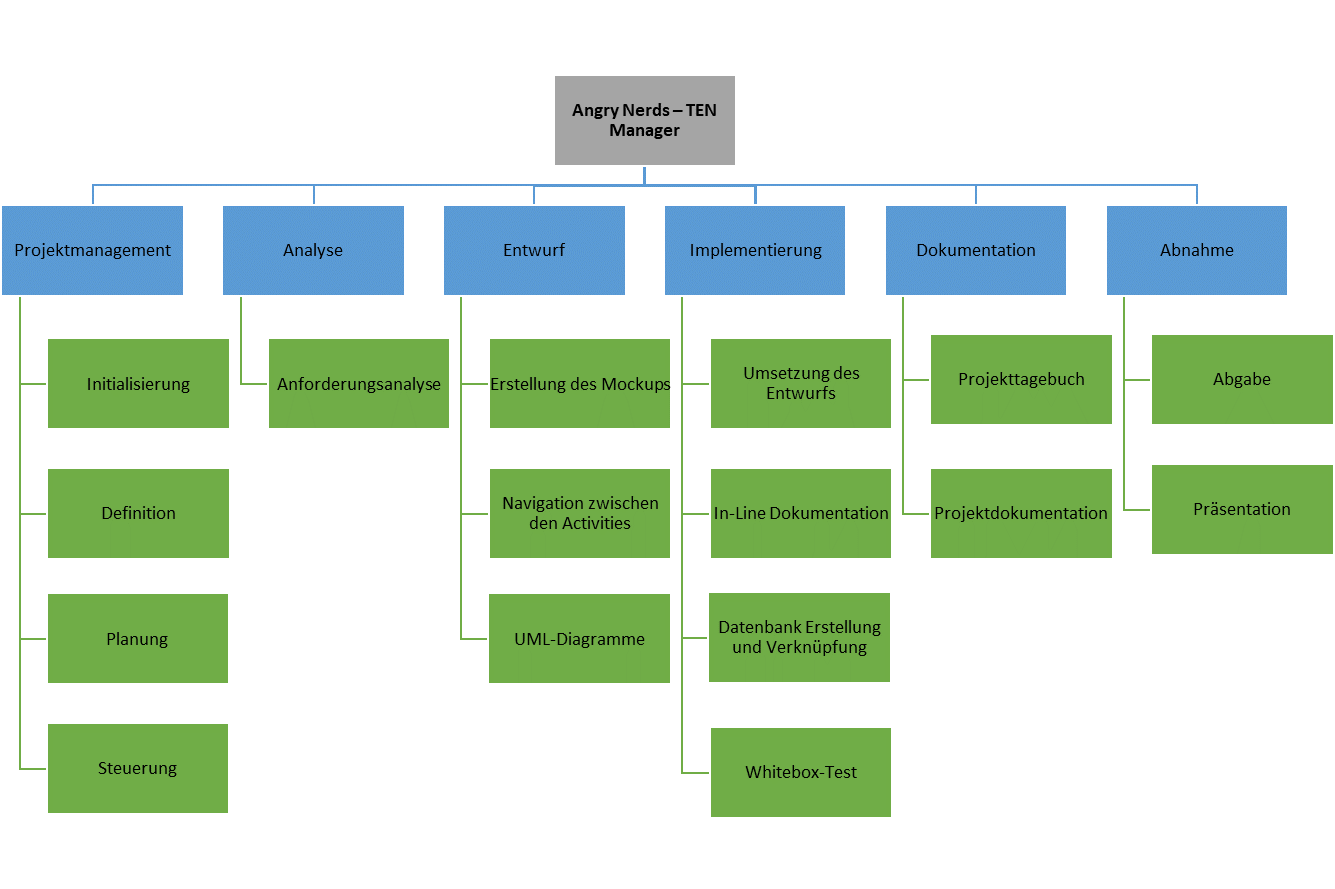
\includegraphics[width=1\textwidth]{img/Projektstrukturplan}\\ % Pfad
\source{Erstellt von Fabia Schmid} % Quelle
\end{minipage}
\end{figure}

\begin{table}[H]
\caption{Meilensteinplan} % Überschrift
\begin{tabular}{|p{2cm}|p{9cm}|p{3cm}|}
\hline
{\textbf{ID}} & {\textbf{Meilenstein}} & {\textbf{Datum}} \\ \hline
1 & Kick-Off gehalten & 05.09.2018 \\ \hline
2 & Vorgehensmodell ausgewählt & 12.09.218 \\ \hline
3 & Datenbankmodel ausgewählt & 14.09.2018 \\ \hline 
4 & Activities verteilt & 20.09.2018 \\ \hline
5 & Mockup fertig & 20.09.2018 \\ \hline
6 & Activities und Layouts fertig & 01.12.2018 \\ \hline
7 & Activities getestet & 10.12.2018 \\ \hline
8 & Activities zusammengeführt & 20.12.2018 \\ \hline
9 & App getestet & 05.01.2019 \\ \hline
10 & Dokumentation fertig & 01.02.2019 \\ \hline
11 & Ausarbeitungsabgabe & 07.02.2019 \\ \hline
12  & Präsentation & 09.02.2019\\ \hline
\end{tabular}
\end{table}

\begin{figure}[H]
\centering
\begin{minipage}[t]{1\textwidth} % Breite, z.B. 1\textwidth		
\caption{GANTT-Diagramm} % Überschrift
\includegraphics[width=1\textwidth]{img/GANTT}\\ % Pfad
\source{Erstellt von Fabia Schmid} % Quelle
\end{minipage}
\end{figure}

\begin{table}[H]
\caption{Geplante Aufgaben} % Überschrift
\begin{tabular}{|p{4cm}|p{10cm}|}
\hline
{\textbf{Name}} & {\textbf{Aufgaben}}  \\ \hline
Ruthild Gilles & Erstellung Service-Klassen,

Schreiben eines Protokolls,

Projekttagebuch führen, 

Dokumentation anfertigen \\ \hline 
Fabia Schmid  & Projektsteuerung und -planung, 

Erstellung der Layouts für die ActivityOverview,  

Erstellung der OnClickListener für die ActivityOverview,  

Projekttagebuch führen, 

Dokumentation anfertigen \\ \hline

Jan Beilfuß & Datenbankzugriffe, 

Start-Up-Lade-Routine von Note, 

Bilderhandling in Note und generell, 

Note-Applicationlogicstrukturierung, 

Projekttagebuch führen, 

Dokumentation anfertigen \\ \hline
Yannick Rüttgers & Erstellung ActivityOverview,  

Planung der Navigation zwischen Klassen, 

Erster Latexentwurfprojekttagebuch, 

Latex-Beauftragter, 

Projekttagebuch führen, 

Dokumentation anfertigen \\ \hline
Robin Menzel & Zusammenführung des Quellcodes, 

Erstellung des Mockups, 

Erstellung der Event Activity, 

Projekttagebuch führen, 

Dokumentation anfertigen \\ \hline
Florian Rath  & Aufteilung der Activities, 

Erstellung Activity ToDo, 

Projekttagebuch führen, 

Dokumentation anfertigen \\ \hline
Joscha Nassenstein & Erstellung von Note, 

Erstellung der TEN-Klassen,  

Erstellung Datendiagramm, 

Projekttagebuch führen, 

Dokumentation anfertigen \\ \hline
Sertan Cetin &  Aufteilung der Activities, 

Erstellung Activity ToDo, 

Projekttagebuch führen, 

Dokumentation anfertigen \\ \hline
\end{tabular}
\end{table}

\newpage
\subsection{Planung der Software}
\subsubsection{Planung des Mock-Ups (Robin Menzel)}
%%%%%%%%%
%Robin
%%%%%%%%%
Das Mockup wurde von Beginn der Projektes an erstellt und ist das Ergebnis vieler Änderungen und Versionen. Während beim ersten Meeting zum Aussehen der App bereits Stilrichtung und Präferenzen der Gruppenmitglieder festgehalten wurden, entstand das erste Mock-Up erst einige Zeit später. Neben Handschriftlichen Zeichnungen zu Beginn des Designs, war das Programm Adobe Xd das ausgewählte Werkzeug für das Mock-Up. Adobe Xd war zu Beginn des Projektes erst in einer Beta Version verfügbar, welche für unsere Ansprüche jedoch ausreichte. Es ist ein vektorbasiertes Tool zum Entwerfen und Prototyping der User Experience für webbasierte und mobile Applikationen.

Das Design leitet sich von Googles Designsprache \textit{Material Design} ab, welche besonders durch die materialartigen, kartenähnlichen Flächen und das Flat Design charakterisiert wird. Außerdem ist das Layout und die Farbgestaltung angelehnt an verschieden Applikationen, wie z.B.
\begin{itemize}
\item Google Notizen
\item Google Kalender
\item Google Fotos
\item Wunderlist
\end{itemize}
Dies liegt vor allem daran, das in diesen Applikationen das Material Design sehr gut umgesetzt wurde. Aus Google Notizen wurde die Übersichtsseite und die charakteristische, schwebende Appbar übernommen. So sind auch unsere TENs in der Übersichtsseite als Fragmente dargestellt, in denen sich die wichtigsten Informationen schnell ablesen lassen. Die Detail- bzw. Bearbeitungsseiten der TENs wurde angelehnt an die Bearbeitungsseite des Google Kalenders. Hier wurden die Kategorien bzw. Einstellmöglichkeiten durch feine Linien visuell voneinander abgetrennt. Durch die eindeutigen Icons und dem auslassen von Beschriftungen wird der Bildschirm optimal genutzt. Auch Wunderlist schafft es in den Detailansichten von ToDos mit wenigen Hinweisen, ein minimalistische, aber ituitive und vorallem infomative Darstellung zu schaffen, von der wir uns inspiriert haben. Bei Google Fotos wurde die untere Navigationsleiste übernommen. So ist es in unserer App nun möglich mit einem Klick zwischen einer Übersicht über alle TENs, zu einer Übersicht über die unterschiedlichen Kategorien zu wechseln. Dies nutzt auf effektive Weise den Platz auf dem Tablet und bietet die Funktion an einer intuitiven Position an. Außerdem können wir so auf einen so genannten Navigation Drawer verzichten, da dieser die Applikation unnötig aufplustert und unsere Applikation kaum Funktionalitäten anbietet, die in diesem Drawer positioniert werden hätte können.

In Adobe Xd lassen sich nicht nur die Oberflächen Designen, sondern auch die User Experience abbilden. So lassen sich Flächen mit einander Verbinden, die nun durch einen Klick geöffnet werden können. Auf diese Art und Weise war es uns möglich Personen aus unserem Umkreis unsere App testen zu lassen. Das Feedback war ausschließlich Positiv. Da wir Elemente aus oft genutzten Apps übernommen haben, stellte die Bedienung unserer App für alle Tester kein Problem dar. Außerdem kam das Feedback, das unsere Oberfläche zur ersten Nutzung einlädt und nicht durch Überladung von Informationen abschreckt.
\begin{figure}[H]
	\subsection*{Übersicht}
	\centering
	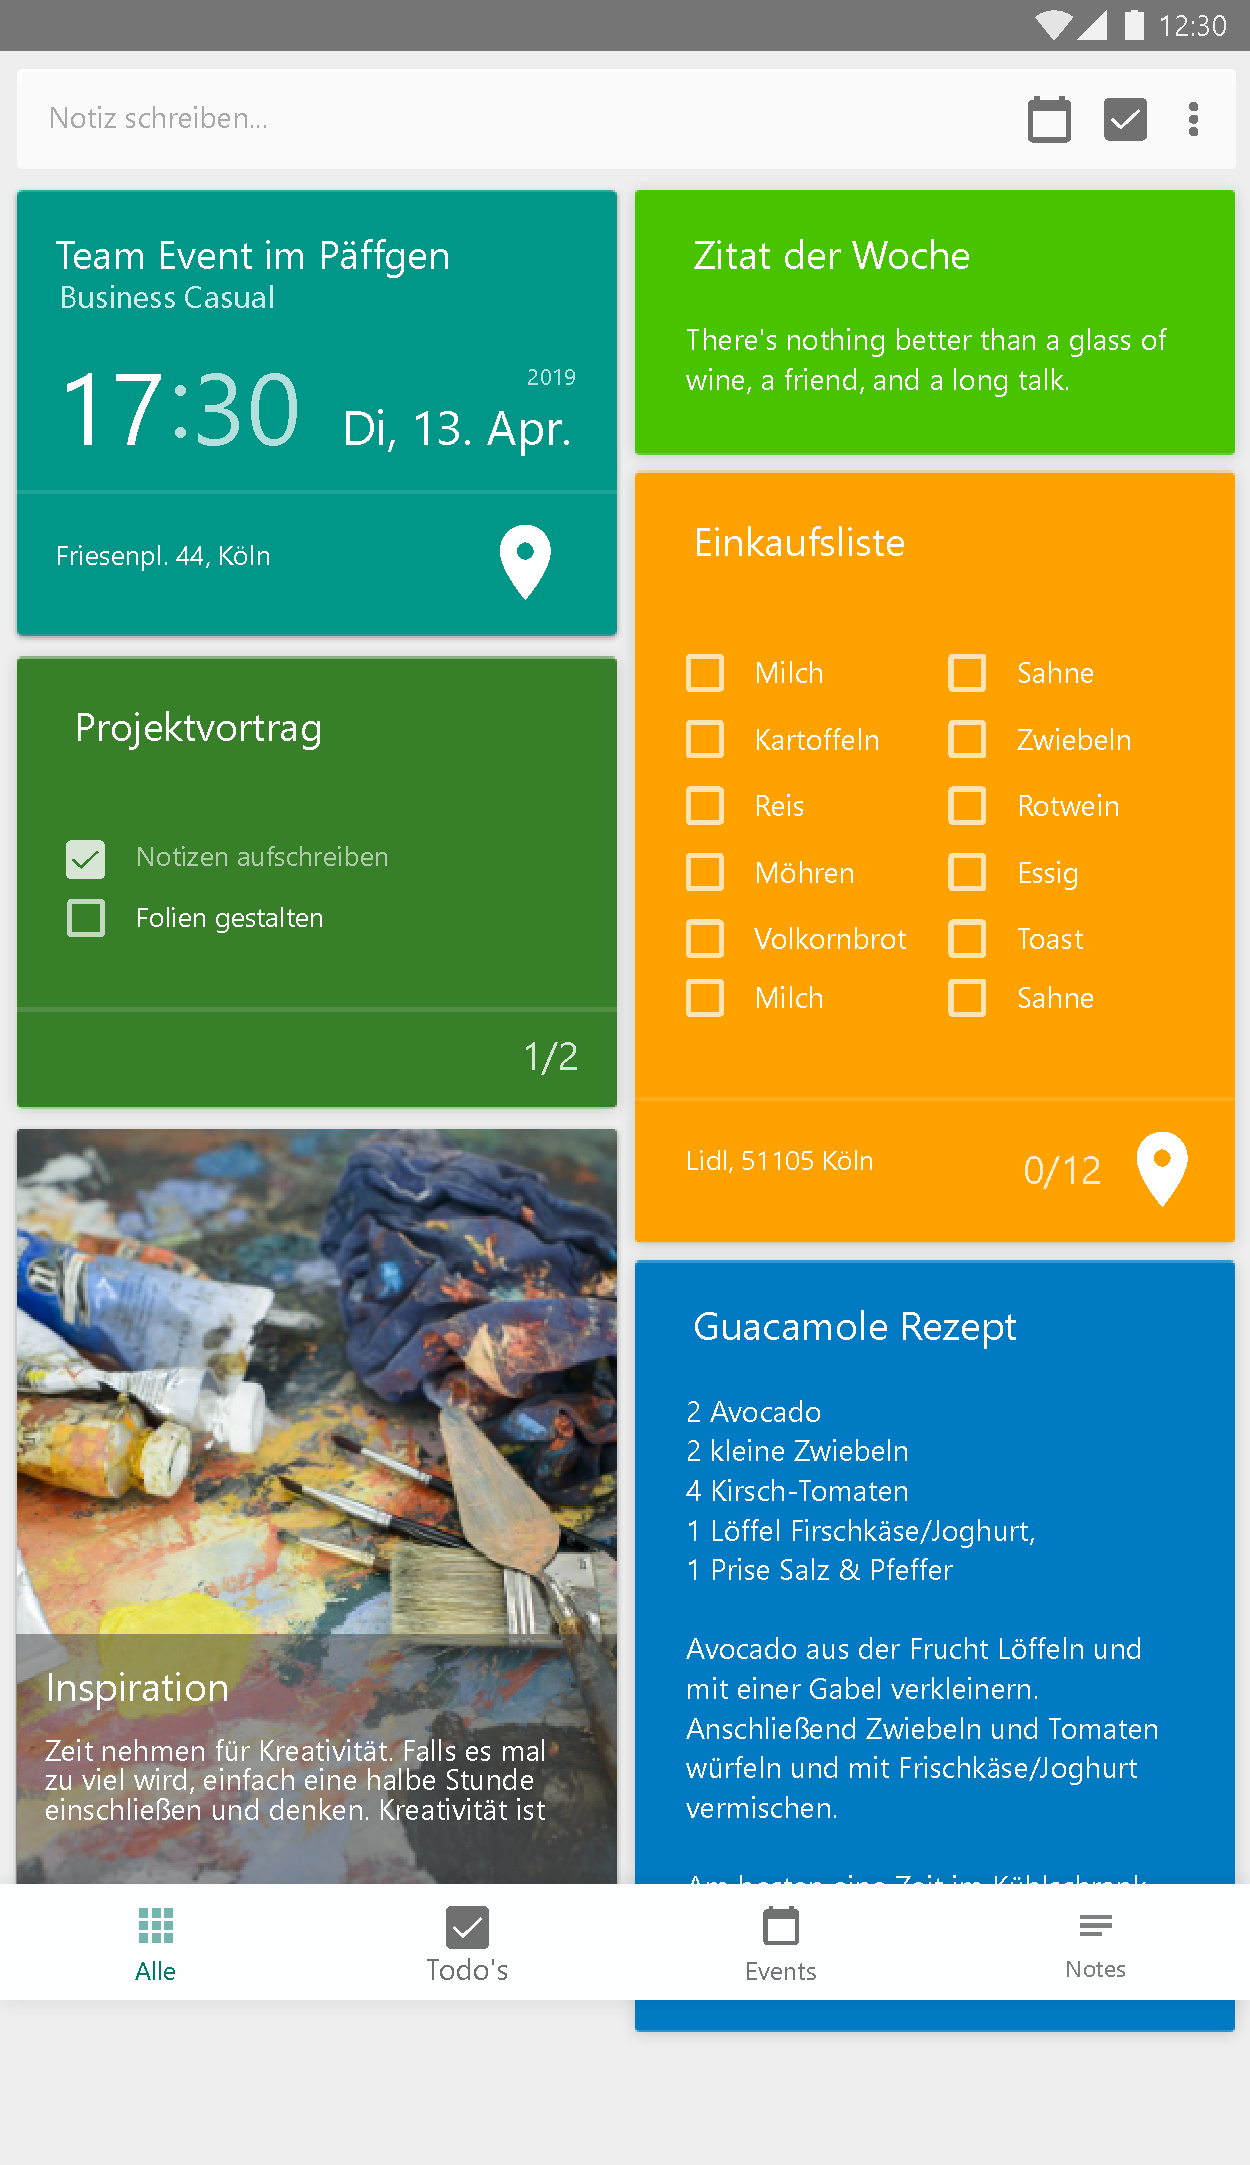
\includegraphics[width=8cm]{img/OverviewActivity.pdf}
	\caption{Mockups - Übersicht über alle TENs}
	\label{img:OverviewActivity}
\end{figure}

\begin{figure}[H]
	\subsection*{Event Activity - Unsere Events}
	\centering
	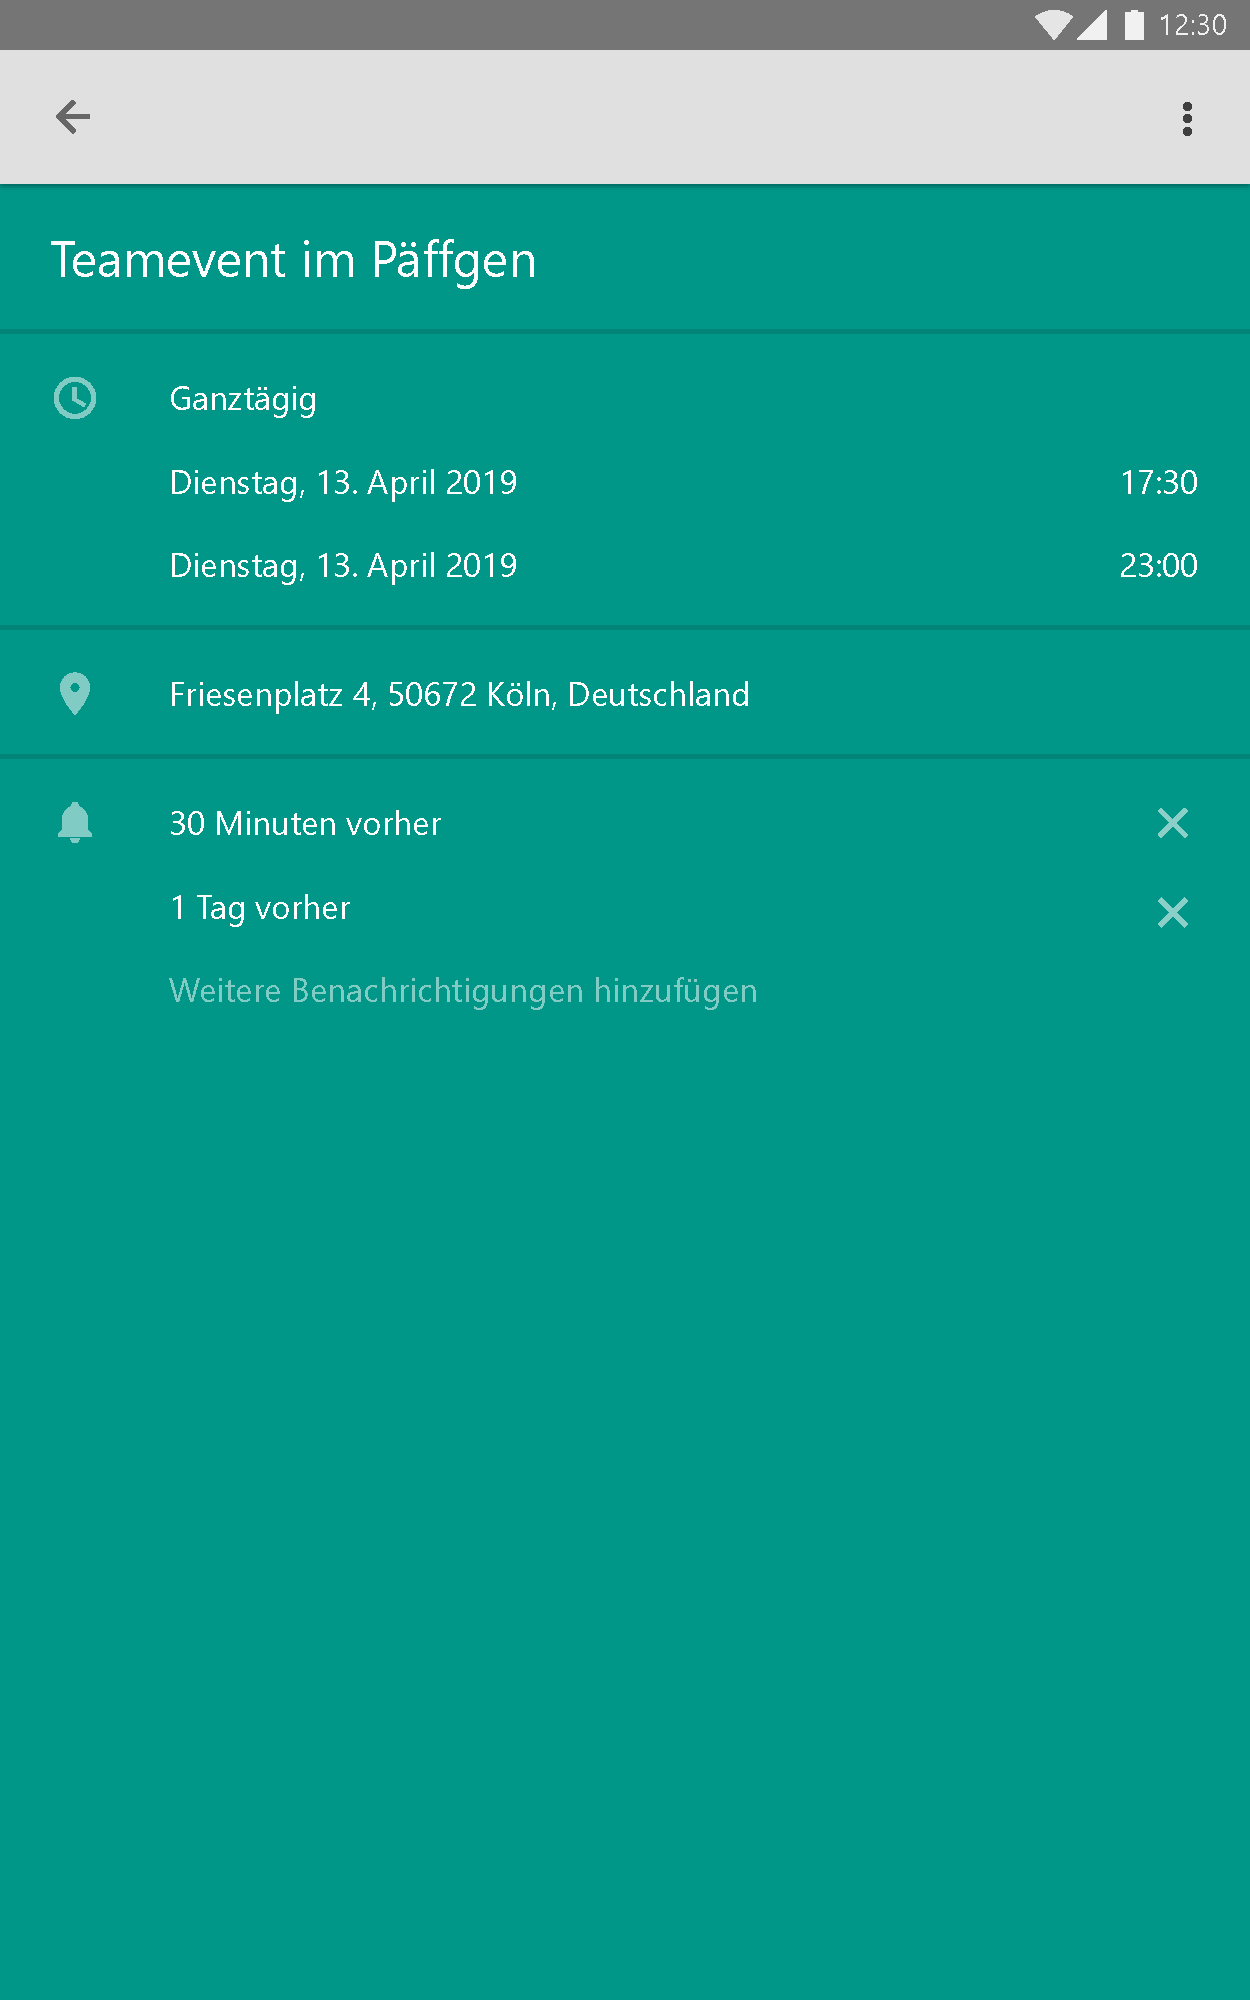
\includegraphics[width=7.25cm]{img/EventActivity.pdf}
	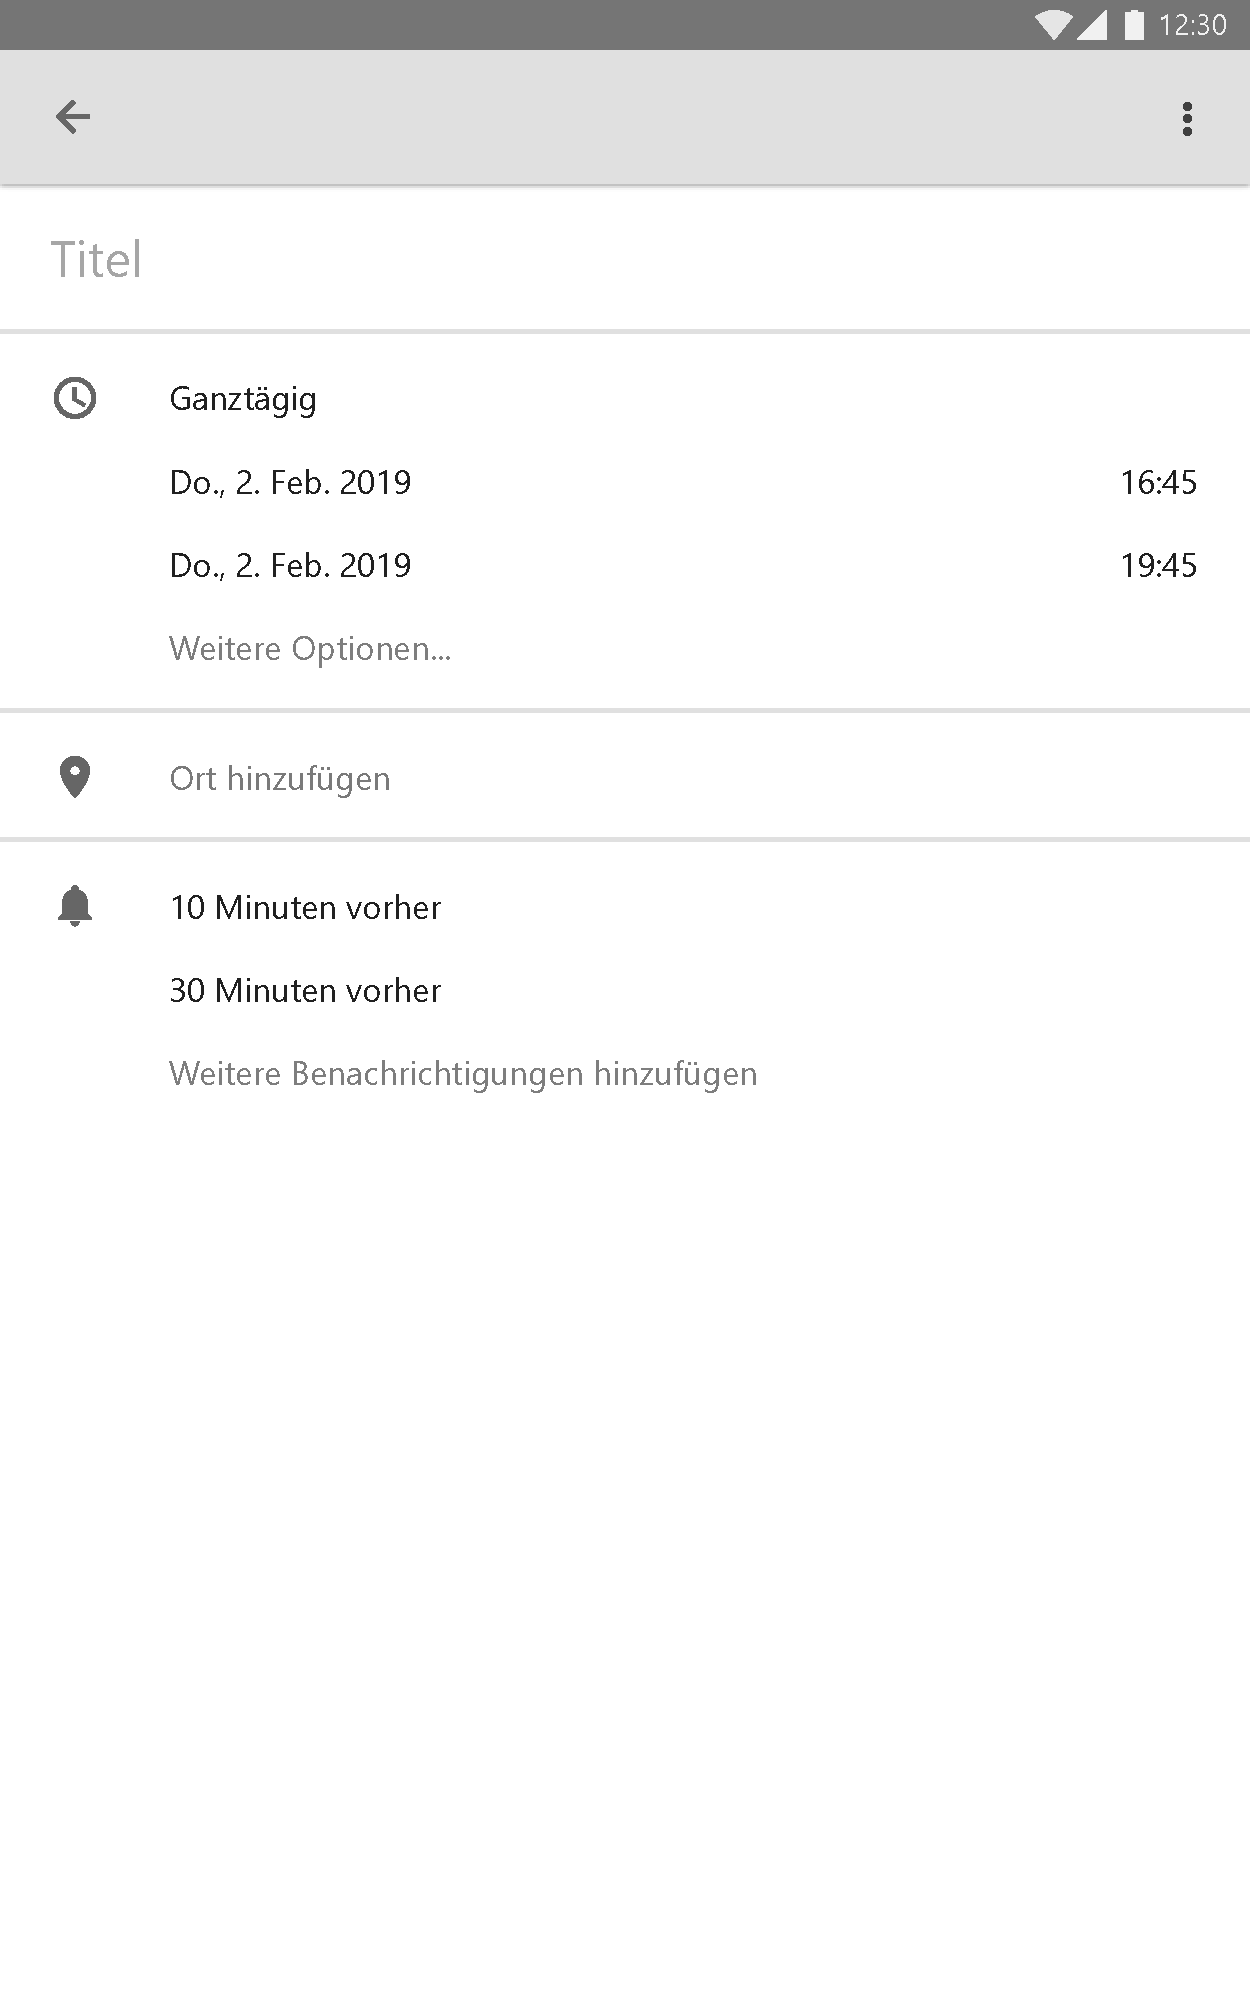
\includegraphics[width=7.25cm]{img/EventActivityNew.pdf}
	\caption{Mockups - Übersicht über ein vorhandenes und ein neues Event}
	\label{img:EventActivity}
\end{figure}

\begin{figure}[H]
	\subsection*{Note Activity - Unsere Notizen}
	\centering
	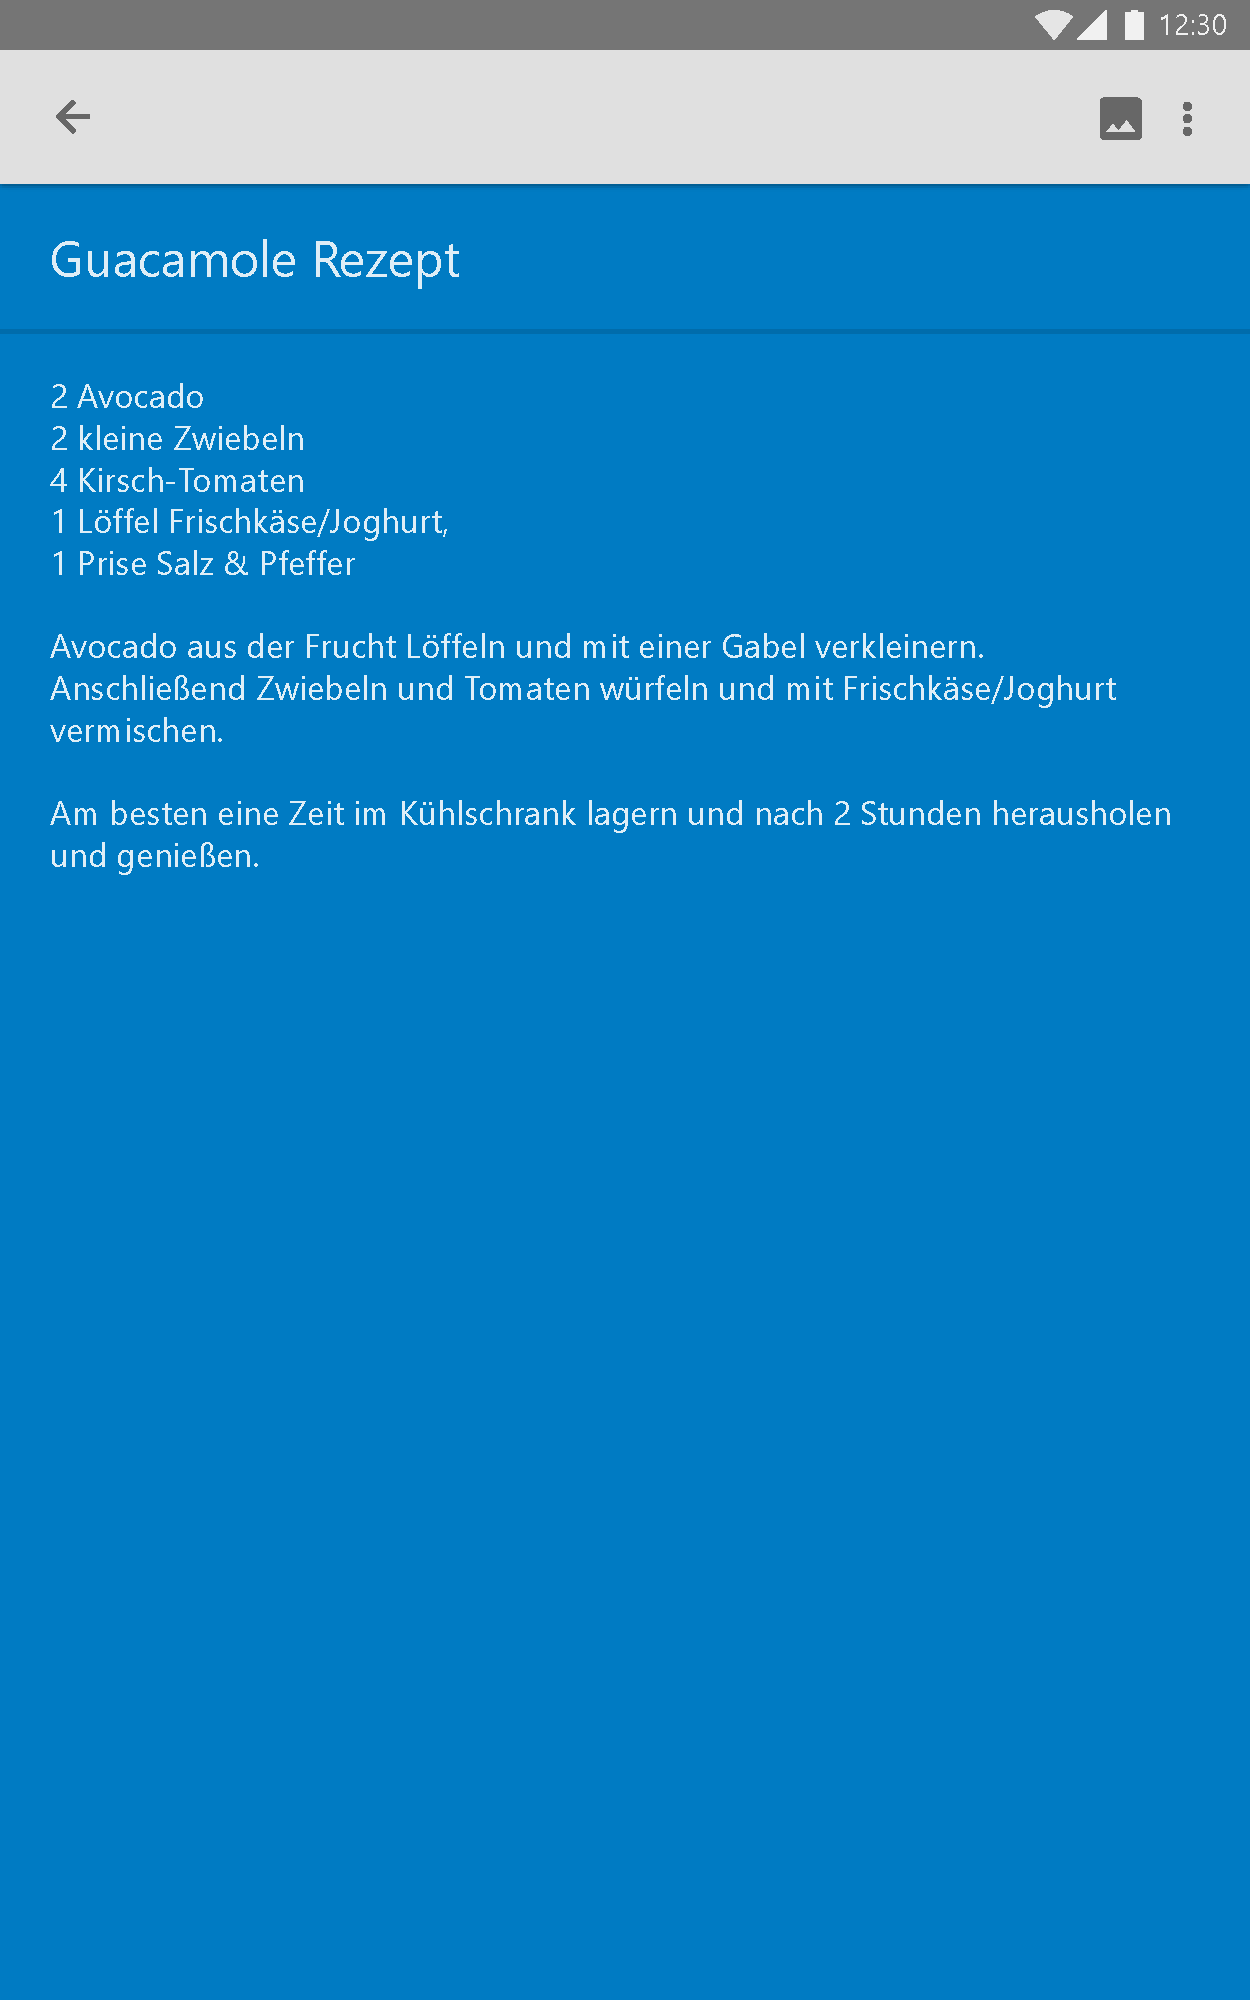
\includegraphics[width=7.25cm]{img/NoteActivity.pdf}
	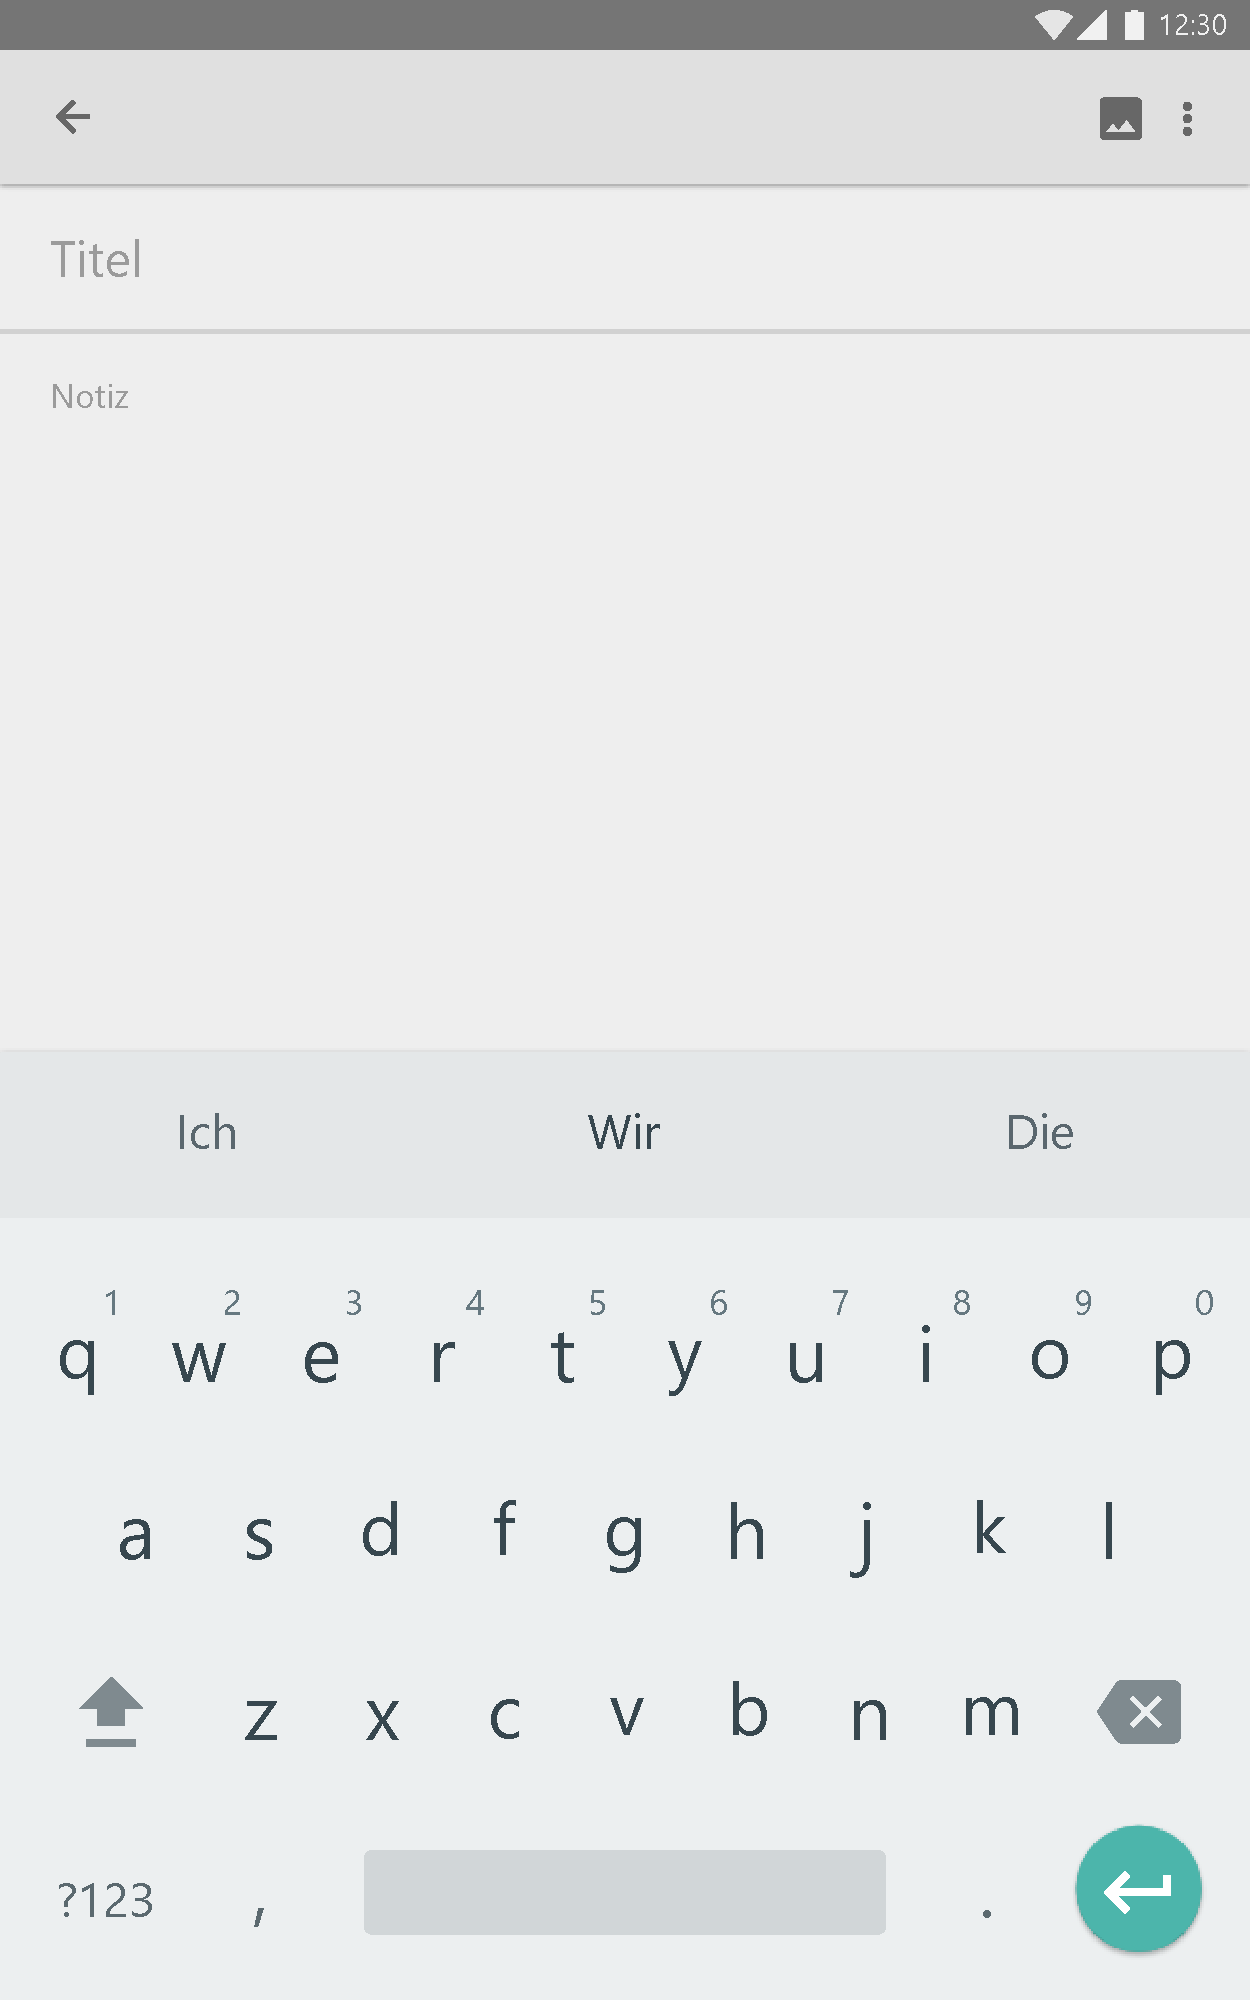
\includegraphics[width=7.25cm]{img/NoteActivityNew.pdf}
	
\includegraphics[width=7.25cm]{img/NoteActivityImage.pdf}
	\caption{Mockups - Übersicht über ein vorhandene, eine leere und eine Bild-Notiz}
	\label{img:NoteActivity}
\end{figure}

\begin{figure}[H]
	\subsection*{Todo Activity - Unsere ToDos}
	\centering
	\includegraphics[width=7.25cm]{img/ToDoActivity.pdf}
	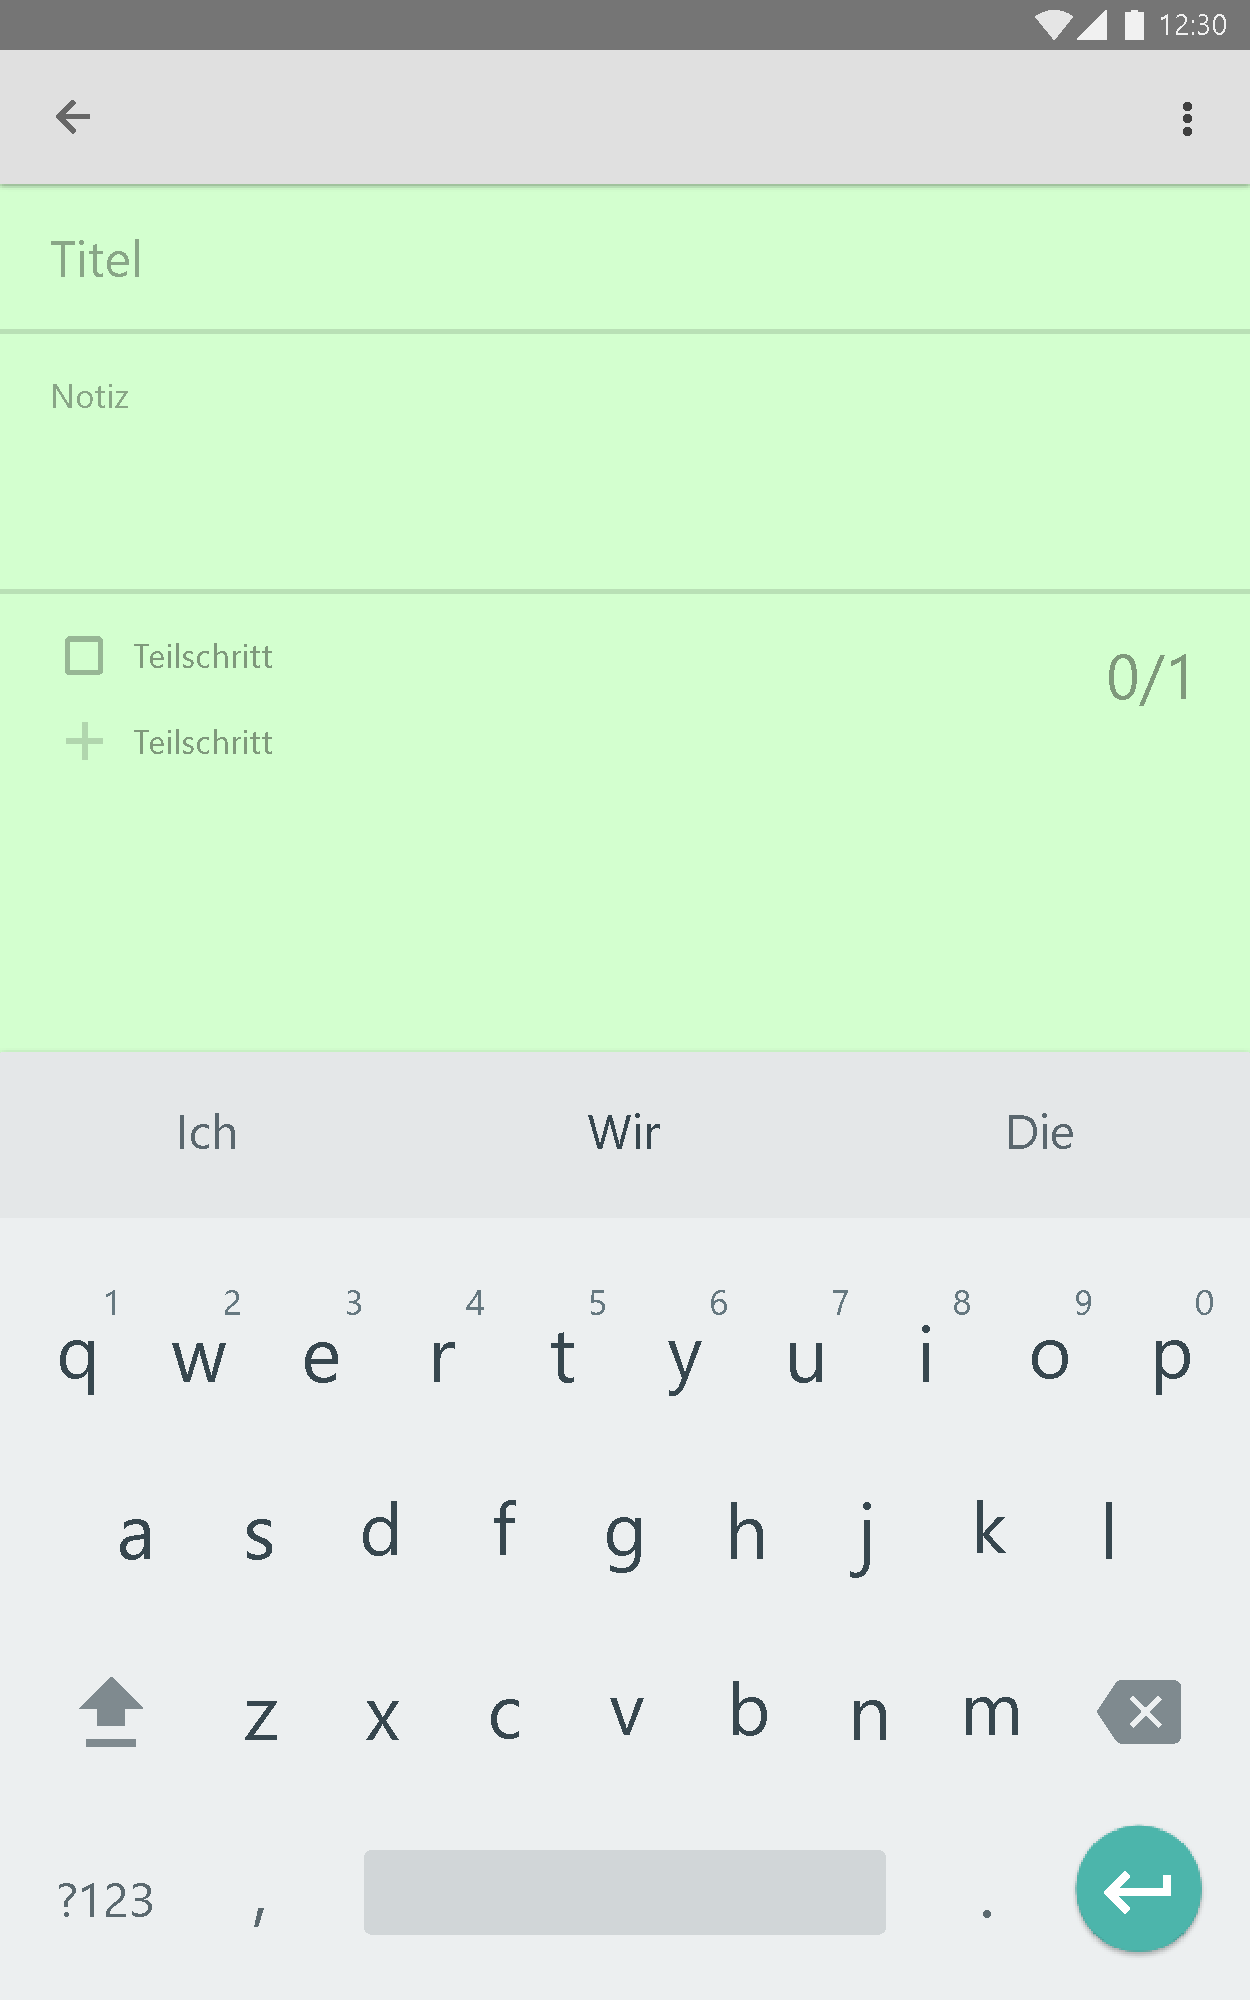
\includegraphics[width=7.25cm]{img/ToDoActivityNew.pdf}
	\caption{Mockups - Übersicht über vorhandene und neue Todos}
	\label{img:ToDoActivity}
\end{figure}

\newpage
\subsubsection{Planung der Datenstruktur und Schnittstellen (Ruthild Gilles)}
%%%%%%%%%
%Ruthild
%%%%%%%%%

Die gewünschte Applikation soll das Managen von Todos, Events und Notes vereinfachen. Anhand der Anforderungen an die Applikation überlegte sich das Datenteam, welche Daten beziehungsweise Informationen in der Datenstruktur der Applikation abgebildet werden sollen. Da sowohl Todo-, Event-, als auch Note-Objekte einheitlich aufgebaut sein sollen, wurde sich dazu entschieden, dass die jeweiligen Klassen von einer TEN-Klasse erben. Alle Todo-, Event- und Note-Objekte benötigen eine ID zu eindeutigen Identifikation des Objektes auf der Datenbank und in der Applikation. Außerdem könnne die Objekte jeweils einen Titel haben. Zudem sollen die verschiedenen Objekte weitere Informationen enthalten. In folgendem Klassendiagramm sind alle geplanten Attribute der Klassen aufgelistet.

\begin{figure}[H]
\centering
\begin{minipage}[t]{1\textwidth} % Breite, z.B. 1\textwidth		
\caption{Klassendiagramm} % Überschrift
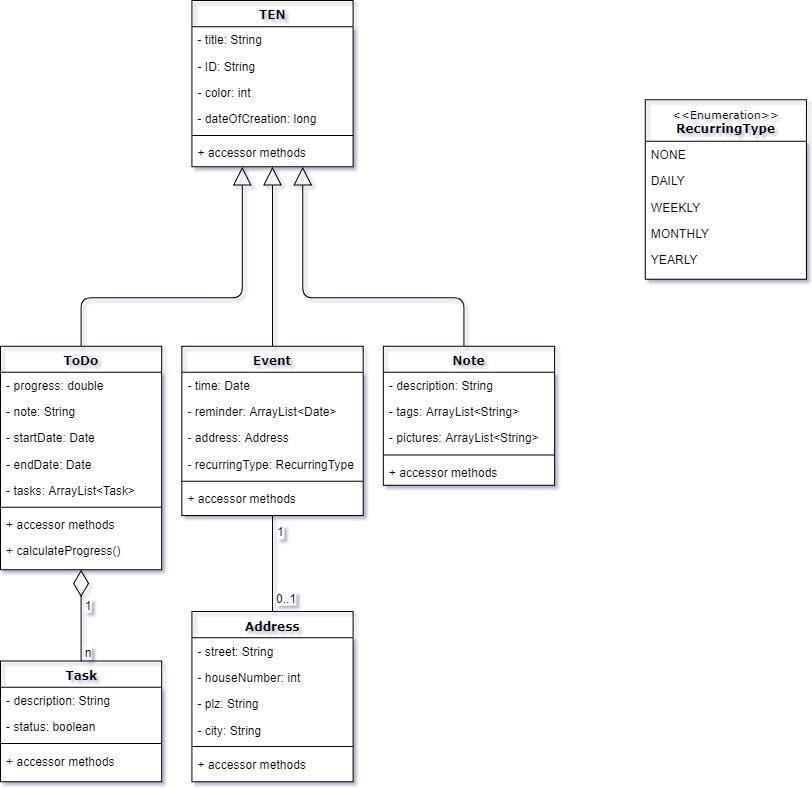
\includegraphics[width=1\textwidth]{img/Klassendiagramm}\\ % Pfad
\source{Erstellt von Joscha Nassenstein} % Quelle
\end{minipage}
\end{figure}

Zusätzlich zu der Struktur der Daten in Form von Klassen mit entsprechenden Attributen wurde ebenfalls die Struktur der Applikation vom Datenteam definiert. Diese ist in nachfolgender Abbildung in einem Systemkontextdiagramm dargestellt.

\begin{figure}[H]
\centering
\begin{minipage}[t]{1\textwidth} % Breite, z.B. 1\textwidth		
\caption{Systemkontextdiagramm} % Überschrift
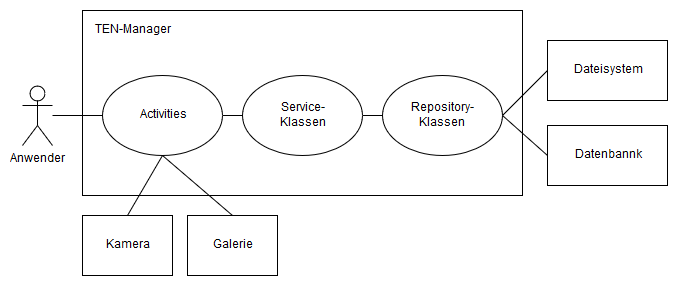
\includegraphics[width=1\textwidth]{img/Systemkontextdiagramm}\\ % Pfad
\source{Erstellt von Ruthild Gilles} % Quelle
\end{minipage}
\end{figure}

Um die Daten auch nach Beendigung der Applikation bei erneutem Starten wieder anzeigen zu können, wurde eine dokumentenbasierte Datenbank an die Applikation angebunden. Auf diese Weise kann eine persistente Datenhaltung erzielt werden. Die einzelnen Activities, welche als Schnittstelle zu den Anwendern dienen, sollen die vom Benutzer eingegebenen Informationen auf der Datenbank speichern können. Dazu sollen Activity-übergreifende Klassen verwendet werden.

Das Datenteam plante die Activity-übergreifenden Klassen und deren Methoden anhand der Anforderungen, der einzelnen Activities. Es sollte möglich sein, einzelne oder auch alle TEN-Objekte von der Datenbank zu erhalten. Auch sollte das Löschen und das Speichern von einzelnen TEN-Objekten möglich sein. Während der Planungsphase wurden hier verschiedene Ansätze in Erwägung gezogen, um diese Anforderungen umzusetzen. Zur Übersichtlichkeit entschied sich das Datenteam letztendlich dafür, einzelne Klassen für jede der vier CRUD-Operationen zu erstellen. Die CRUD-Operationen beinhalten das Erstellen (Create), das Lesen (Read), das Aktualisieren (Update) und das Löschen (Delete) von einzelnen Objekten. Die einzelnen Methoden der CRUD-Klassen sind in folgender Abbildung dargestellt.

\begin{figure}[H]
\centering
\begin{minipage}[t]{1\textwidth} % Breite, z.B. 1\textwidth		
\caption{CRUD-Klassen} % Überschrift
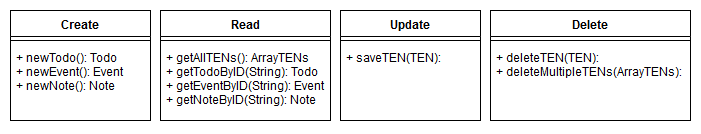
\includegraphics[width=1\textwidth]{img/CRUD-Klassen}\\ % Pfad
\source{Erstellt von Ruthild Gilles} % Quelle
\end{minipage}
\end{figure}

Da der Aufwand für die Umsetzung aller geforderten Anforderungen zu Projektstart lediglich grob geschätzt werden konnte, definierte das Datenteam abgesehen von der Schnittstelle zur Datenbank noch einige weitere Schnittstellen. Die Implementierung dieser weiteren Schnittstellen wurde nicht in den Anforderungen gefordert und würde nur bei genug Zeitüberschuss umgesetzt werden. Zu den weiteren optionalen Schnittstellen gehören das Exportieren von Todos, Events und Notes in die Zwischenablage oder auch in andere Applikationen, die auf dem entsprechenden Endgerät installiert sind. Für ein Event soll es die Möglichkeit geben eine Adresse hinzuzufügen. Hier wäre eine weitere optionale Schnittstelle die Verknüpfung mit Google Maps. Auch könnte eine Schnittstelle zu einer anderen Kalender App implementiert werden, in die ein Event exportiert werden könnte.

\newpage

\subsubsection{Planung der Activities und Layouts (Florian Rath)}
%%%%%%%%%
%Florian
%%%%%%%%%

Hier den Text einfach hin kopieren.

\subsubsection{Planung der Navigation zwischen den Activities (Yannick Rüttgers)}
%%%%%%%%%
%Yannick
%%%%%%%%%

Hier den Text einfach hin kopieren.

\subsection{Geplante Aufgabenverteilung im Team (Fabia Schmid)}
%%%%%%%%%
%Fabia
%%%%%%%%%

Hier den Text einfach hin kopieren.

%%%%%%%%%%%%%%%%%%%%%%%%%%%%%%%%%%%%%%%%%%%%%%%%%%%%%
%Als Beispiel
%Bitte noch entfernen:

So kann man Abbildungen einfügen:

\begin{figure}[H]
\centering
\begin{minipage}[t]{1\textwidth} % Breite, z.B. 1\textwidth		
\caption{Abbildungsbeschriftung} % Überschrift

\includegraphics[width=1\textwidth]{img/fhdw}\\ % Pfad
\source{\url{http://dominique-fleury.com/?p=302}} % Quelle
\end{minipage}
\end{figure}


%!TEX root = ../Thesis.tex
\section{Beschreibung des Projektverlaufs}
\fancyhead[R]{Beschreibung des Projektverlaufs}
\label{instal}

\subsection{Tatsächliche Aufgabenverteilung im Team (Fabia Schmid)}
%%%%%%%%%%%
%Fabia
%%%%%%%%%%%

\begin{figure}[H]
\centering
\begin{minipage}[t]{1\textwidth} % Breite, z.B. 1\textwidth		
\caption{Tatsächliche Aufgabenverteilung} % Überschrift

\includegraphics[width=1\textwidth]{img/fhdw}\\ % Pfad
\source{Erstellt von Fabia Schmid} % Quelle
\end{minipage}
\end{figure}

Hier den Text einfach hin kopieren.

\subsection{Teammeetingprotokolle}
%%%%%%%%%%%
%Ruthild
%%%%%%%%%%%

Hier den Text einfach hin kopieren.

\subsection{Projekttagebücher aller Teammitglieder}
%%%%%%%%%%%
%Ruthild
%%%%%%%%%%%
\subsubsection{Projekttagebuch Jan Beilfuß}
\begin{longtable}{|p{10cm}|p{2cm}|p{2cm}|}
\hline
{\textbf{Beschreibung}} & {\textbf{Dauer}} & {\textbf{Datum}} \\ \hline

\end{longtable}

\newpage
\subsubsection{Projekttagebuch Joscha Nassenstein}
\begin{longtable}{|p{10cm}|p{2cm}|p{2cm}|}
\hline
{\textbf{Beschreibung}} & {\textbf{Dauer}} & {\textbf{Datum}} \\ \hline

\end{longtable}

\newpage
\subsubsection{Projekttagebuch Fabia Schmid}
\begin{longtable}{|p{10cm}|p{2cm}|p{2cm}|}
\hline
{\textbf{Beschreibung}} & {\textbf{Dauer}} & {\textbf{Datum}} \\ \hline
Aufgabe lesen und verstehen & 30 min & 05.09.2018 \\ \hline
Kick-Off Meeting zur Besprechung der Aufgabe, Verteilung der Rollen & 50 min & 05.09.2018 \\ \hline
Erstellung eines Meilensteinplans & 50 min & 05.09.2018 \\ \hline
Vorstellung des Meilensteinplans und Besprechung der anderen Ergebnisse & 40 min & 05.09.2018 \\ \hline
Aufarbeitung der Abgabetermine und Information der Gruppenteilnehmer  & 20 min & 10.09.2018 \\ \hline
Installation von Latex & 120 min & 10.09.2018 \\ \hline
Festlegung des Vorgehensmodells, durch Abwägung von Vor- und Nachteilen der verschiedenen Modelle (Ergebnis: Erweitertes Wasserfallmodell)
 & 40 min & 11.09.2018 \\ \hline
Teammeeting & 60 min & 22.09.2018 \\ \hline
Github Anmeldung und Einbindung des Projektes & 60 min & 13.10.2018 \\ \hline
Entwicklung des Layouts für das „Event“  & 70 min & 20.10.2018 \\ \hline
Entwicklung des Layouts für das „Note“ & 60 min & 21.10.2018 \\ \hline
Recherche über Listen, Checkboxen und Verwendung von mehreren Layouts & 50 min & 21.10.2018 \\ \hline
Besprechung der Layouts (Aufbau, etc.) & 50 min & 27.10.2018 \\ \hline
Entwicklung des Layouts für das „ToDo“ & 40 min & 27.10.2018 \\ \hline
Erstellung des Projekttagebuch mit Latex & 40 min & 30.10.2018 \\ \hline
Zusammentragung der momentanen Projektstände und Abschätzung, ob die Meilensteine erreicht werden können & 30 min & 17.11.2018 \\ \hline
Neuplanung eines Meilensteins und Abstimmung mit dem Team & 20 min & 26.11.2018 \\ \hline
Teammeeting & 50 min & 04.12.2018 \\ \hline
Koordination der anzufertigen Diagramme und Entwicklungsstand überprüfen& 10 min & 04.12.2018 \\ \hline
Entwicklung des Layouts für das „Image“ & 20 min & 12.12.2018 \\ \hline
Entwicklung des Layouts für die Overview &  60 min & 02.01.2019 \\ \hline
Aufteilung der Ausarbeitung & 20 min & 02.01.2019 \\ \hline
Entwicklung des Layouts für das Bedienleisten-Fragment & 20 min & 04.01.2019 \\ \hline
Meilenstein Umplanung & 10 min & 15.01.2019 \\ \hline
Erinnerung an die Erstellung der Kapitel der Ausarbeitung & 10 min & 23.01.2019 \\ \hline
Dokumentation & 240 min & 03.02.2019 \\ \hline
\end{longtable}
Summe in Minuten: 1270

\newpage
\subsubsection{Projekttagebuch Florian Rath}
\begin{longtable}{|p{10cm}|p{2cm}|p{2cm}|}
\hline
{\textbf{Beschreibung}} & {\textbf{Dauer}} & {\textbf{Datum}} \\ \hline

\end{longtable}

\newpage
\subsubsection{Projekttagebuch Robin Menzel}
\begin{longtable}{|p{10cm}|p{2cm}|p{2cm}|}
\hline
{\textbf{Beschreibung}} & {\textbf{Dauer}} & {\textbf{Datum}} \\ \hline
Aufgabe lesen und verstehen & 30 min & 05.09.2018 \\ \hline
Kick-Off Meeting zur Besprechung der Aufgabe, Verteilung der Rollen & 50 min & 05.09.2018 \\ \hline
Konzeption eines Mockups und den Activities & 50 min & 05.09.2018 \\ \hline
Besprechung der in Aufgabenteilung entstandenen Ergebnisse & 40 min & 05.09.2018 \\ \hline
Installation von Adobe XD für MockUps & 20 min & 05.09.2018 \\ \hline
Installation und Einrichtung von Git & 20 min & 05.09.2018 \\ \hline
Erstellung und Einrichtung eines GitHub Repositorys & 40 min & 05.09.2018 \\ \hline
Erstellung von MockUps in der ersten Version & 180 min & 06.09.2018 \\ \hline
Wahl der LateX Distribution & 20 min & 10.09.2018 \\ \hline
Installation von LateX & 120 min & 10.09.2018 \\ \hline
Projekttagebuch pflegen & 10 min & 11.09.2018\\ \hline
Weiterentwicklung des MockUps & 30 min & 15.09.2018\\ \hline
Meeting zur Besprechung der Ergebnisse aus dem Design- und Daten-Team & 60 min & 22.09.2018\\ \hline
Korrekturen am MockUp und Teilen der Ergebnisse im Microsoft Teams & 30 min & 23.09.2018\\ \hline
Kommunikation mit Data Team im Bezug auf Objekte und Übergabe an Activities & 30 min & 23.10.2018 \\ \hline
Erstellung des XML-Layouts der Event-Activity & 180 min & 27.10.2018\\ \hline
Recherche und Design von Farben für die Hintergründe von Activities und Erstellung von res-Files & 60 min & 28.10.2018\\ \hline
Probleme im Git Repository beheben und einrichten von Branches & 30 min & 28.10.2018\\ \hline
Erstellung des Projekttagebuchs in Latex & 40 min & 30.10.2018 \\ \hline
Weiterentwicklung des XML-Layouts der Event-Activity & 120 min & 15.10.2018\\ \hline
Recherche Umsetzung der Datumsauswahl (DatePicker) & 60 min & 15.10.2018\\ \hline
Git Repository neu aufsetzen (Merger und neu anlegen) & 180 min & 01.12.2018\\ \hline
Teammeeting & 50 min & 04.12.2018\\ \hline
Erstellung Notwendiger Klassen für die Event Activity & 600 min & 10.12.2018 \\ \hline
Recherche nach App oder Toolbar für API 19 & 120 min & 12.12.2018 \\ \hline
Implementation einer Toolbar für alle TENs & 260 min & 13.12.2018 \\ \hline
Implementation des 3-Punkt-Menüs in der Toolbar & 30 min & 13.12.2018 \\ \hline
Implementation des Öffnens der Activity (Öffnen mit ID, ohne, Übergänge) & 90 min &  17.12.2018\\ \hline
Erstellung des Projekttagebuchs in Latex & 15 min & 19.12.2018 \\ \hline
Recherche DialogPicker um Zeit und Datum für Events auszuwählen & 120 min & 23.12.2018 \\ \hline
Implementation von Date- und Time-Picker & 300 min & 27.12.2018 \\ \hline
Implementation der dynamischen Reminder in der GUI und dem Auswahldialog & 390 min & 29.12.2018 \\ \hline
Recherche Notification Service und Alarm Manager & 90 min & 30.12.2019 \\ \hline
Implementation von Remindern inkl. Notification Service und Alarm Manager & 120 min & 31.01.2019 \\ \hline
Ausführliches Testen 05.01.2019 & 120 min & 04.01.2019\\ \hline
Anpassungen auf API 19 & 120 min & 05.01.2019 \\ \hline
Ausführliches Testen 09.01.2019 & 90 min & 10.01.2019\\ \hline
Anpassungen an dem Alarm Manager um Reminder vor aktueller Zeit zu ignorieren & 30 min & 10.01.2019 \\ \hline
Recherche nach Schnittstellen zu Google Maps & 15 min & 10.01.2019 \\ \hline
Implementation eines Buttons um die Adresse eines Events in Google Maps zu öffnen & 30 min 6 & 10.01.2019 \\ \hline
GUI Anpassungen für den Navigations-Button & 30 min & 11.01.2019 \\ \hline
Implementation einer Teilen-Funktionalität für Text-basiertes Event & 45 min & 13.01.2019 \\ \hline
Implementation einer Export-Funktion in andere Kalender Applikationen & 30 min & 13.01.2019 \\ \hline
Implementation der Wiederholungsfunktion (Einmalig, Täglich, ...) & 180 min & 17.01.2019 \\ \hline
Erstellung der Dokumentation 1 & 120 min & 28.01.2019 \\ \hline
Erstellung des Projekttagebuchs in Latex & 60 min & 29.12.2018 \\ \hline
Erstellung der Dokumentation 2 & 140 min & 30.01.2019 \\ \hline
\end{longtable}
Summe in Minuten: 4595

\newpage
\subsubsection{Projekttagebuch Ruthild Gilles}
\begin{longtable}{|p{10cm}|p{2cm}|p{2cm}|}
\hline
{\textbf{Beschreibung}} & {\textbf{Dauer}} & {\textbf{Datum}} \\ \hline
Aufgabe lesen und verstehen & 30 min & 05.09.2018 \\ \hline
Kick-Off Meeting zur Besprechung der Aufgabe, Verteilung der Rollen & 50 min & 05.09.2018 \\ \hline
Festlegung des Umfangs (Muss/Kann Kriterien) & 50 min & 05.09.2018 \\ \hline
Besprechung der in Aufgabenteilung entstandenen Ergebnisse & 40 min & 05.09.2018 \\ \hline
Installation von LateX & 120 min & 10.09.2018 \\ \hline
Projekttagebuch ausfüllen & 10 min & 11.09.2018 \\ \hline
Erstellung des Datenmodells & 50 min & 15.09.2018 \\ \hline
Teammeeting & 60 min & 22.09.2018 \\ \hline
Überlegung Aufgabenteilung, Aufgabenvergabe und Erklärung dieser bezogen auf die MainActivity & 40 min & 09.10.2018 \\ \hline
Installation und Einrichtung von GIT & 30 min & 13.10.2018 \\ \hline
Teammeeting Data-Team &  60 min & 26.10.2018 \\ \hline
Klonen des Data-Branches von GIT & 120 min & 27.10.2018 \\ \hline
Deklaration von gettern und settern für Datenobjekte & 120 min & 28.10.2018 \\ \hline
Projekttagebuch ausfüllen & 20 min & 31.10.2018 \\ \hline
Entwicklung von SetterService Klasse & 180 min & 16.11.2018 \\ \hline
Teammeeting Data-Team & 100 min & 20.11.2018 \\ \hline
Entwicklung von Service Klassen & 120 min & 21.11.2018 \\ \hline
Überlegung neuer Struktur für Services & 90 min & 22.11.2018 \\ \hline
Implementierung neuer Service-Struktur & 120 min & 30.11.2018 \\ \hline
Einbindung der Mockdaten & 80 min & 01.12.2018 \\ \hline
Implementierung weiterer Teile neuer Struktur & 90 min & 02.12.2018 \\ \hline
Änderungen an neuer Service-Struktur & 40 min & 03.12.2018 \\ \hline
Teammeeting & 50 min & 04.12.2018 \\ \hline
Entwicklung von Create-Klasse & 60 min & 04.12.2018 \\ \hline
Änderungen an Update-Klasse & 40 min & 17.12.2018 \\ \hline
Projekttagebuch ausfüllen & 20 min & 18.12.2018 \\ \hline
Bugfixing in Update- und Read-Klasse & 90 min & 02.01.2019 \\ \hline
Mockdaten durch Zugriff auf Datenbank ersetzt & 60 min & 02.01.2019 \\ \hline
Ergänzung einer Methode in Delete-Klasse & 30 min & 04.01.2019 \\ \hline
Neue Farben für GUI festlegen & 30 min & 07.01.2019 \\ \hline
Latex - Vorlage anpassen & 120 min & 14.01.2019 \\ \hline
Latex - Struktur für Ausarbeitung erstellen & 120 min & 18.01.2019 \\ \hline
Meinen Teil der Ausarbeitung schreiben & 180 min & 28.01.2019 \\ \hline
Latex - Meetingprotokolle einfügen & 180 min & 01.02.2019 \\ \hline
Latex - Quellcode einfügen & 120 min & 03.02.2019 \\ \hline
Latex - Ausarbeitungen der anderen einfügen & 180 min & 03.02.2019 \\ \hline
Projekttagebuch ausfüllen & 20 min & 03.02.2019 \\ \hline
Latex - Projekttagebücher einfügen & 120 min & 03.02.2019 \\ \hline
\end{longtable}
Summe in Minuten: 3090

\newpage
\subsubsection{Projekttagebuch Sertan Cetin}
\begin{longtable}{|p{10cm}|p{2cm}|p{2cm}|}
\hline
{\textbf{Beschreibung}} & {\textbf{Dauer}} & {\textbf{Datum}} \\ \hline

\end{longtable}

\newpage
\subsubsection{Projekttagebuch Yannick Rüttgers}
\begin{longtable}{|p{10cm}|p{2cm}|p{2cm}|}
\hline
{\textbf{Beschreibung}} & {\textbf{Dauer}} & {\textbf{Datum}} \\ \hline

\end{longtable}

\newpage
\subsection{Beschreibung von Problemen}
%%%%%%%%%%%
%Fabia
%%%%%%%%%%%

Im Lauf des Projektes konnten zwei Meilensteine nicht fristgerecht erfüllt werden. Einmal die Fertigstellung der Activities und die Fertigstellung der Dokumentation.
 
Die Fertigstellung der Activities und der Layouts war für den 01.12.2018 geplant, konnte jedoch nicht fristgerecht fertiggestellt werden, da projektfremde Tätigkeiten die Umsetzung verzögerten. Beispielsweise schrieben wir eine Klausur, die bei der Projektplanung noch nicht bekannt war. Als Ergebnis wurde der Meilenstein auf ein späteres Datum geplant und konnte danach fristgerecht erfüllt werden. Diese Verschiebung hatte jedoch keinen negativen Einfluss auf die Fertigstellung des Projektes.

Auch der Meilenstein „Dokumentation fertig“ konnte nicht fristgerecht zum 01.02.2019 erreicht werden. Auch in diesem Fall waren projektfremde Tätigkeiten die Ursache für den Verzug. Jedoch musste der Meilenstein nur um 3 Tage verschoben werden, wodurch das Projektergebnis nicht gefährdet wurde.

Weitere Probleme oder Verzögerungen traten nicht auf und das Projekt konnte erfolgreich am 09.02.2019 vorgestellt werden.




%!TEX root = ../Thesis.tex
\section{Dokumentation der Software}
\fancyhead[R]{Dokumentation der Software}
\label{instal}

\subsection{Dokumentation der Paketstruktur (Sertan Cetin)}
%%%%%%%%%%%
%Sertan
%%%%%%%%%%%
Die entwickelte App ist innerhalb des Paketes com.example.robin.angrynerds-wip in mehrere Klassen unterteilt. Zu jeder Activity gehören mehrere Klassen. Um die Übersichtlichkeit zu steigern, wurden die Klassen und Activities in Ordnern untergebracht. Die gesamte Ordnerstruktur sieht wie folgt aus:

\begin{figure}[H]
\centering
\begin{minipage}[t]{1\textwidth} % Breite, z.B. 1\textwidth		
\caption{Paketstruktur} % Überschrift
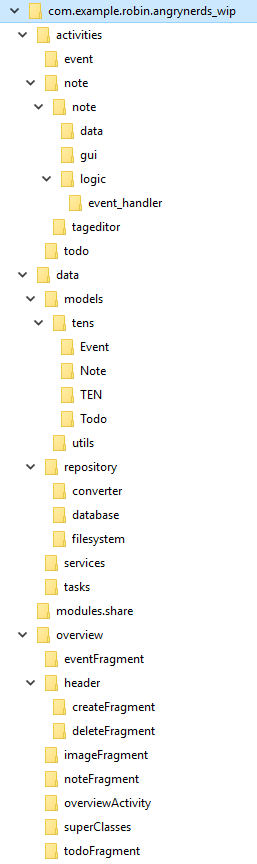
\includegraphics[width=5.5cm]{img/Projektordnerstruktur}\\ % Pfad
\source{Erstellt von Sertan Cetin} % Quelle
\end{minipage}
\end{figure}

Das Paket beinhaltet insgesamt fünf Activities mit jeweils einer ApplicationLogic, Gui und Data.

\begin{figure}[H]
\centering
\begin{minipage}[t]{1\textwidth} % Breite, z.B. 1\textwidth		
\caption{Paketstruktur} % Überschrift
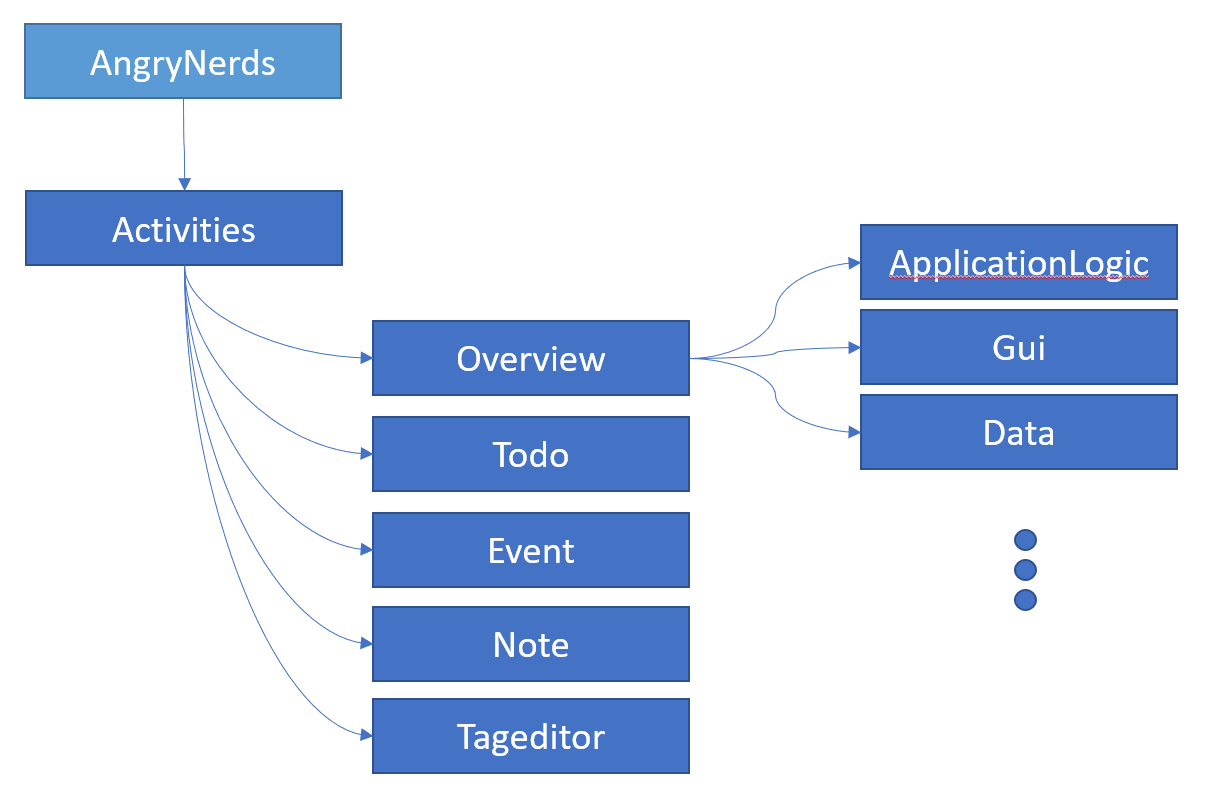
\includegraphics[width=1\textwidth]{img/Paketstruktur}\\ % Pfad
\source{Erstellt von Sertan Cetin} % Quelle
\end{minipage}
\end{figure}


\subsection{Dokumentation der Activities}
%%%%%%%%%%%
%Alle
%%%%%%%%%%%

\subsubsection{Main Activity}
%Yannick
\textbf{Aufgabe und Funktionen (Yannick Rüttgers)}\\
Die in diesem Kapitel erläuterte Activity Overview dient dem Nutzer als Einstiegspunkt in die Applikation. Von hier aus werden alle weiteren Activities aufgerufen.

Wenn der Nutzer die Applikation startet, sieht er als erstes diese Activity. Diese enthält alle bereits erstellten TENs in Kachelform mit einigen Infos. Die Kacheln sind in einer oder mehreren Spalten, je nach Größe des Displays angeordnet. Diese Kacheln sind scrollbar.

Am unteren Bildschirmrand hat der Nutzer die Möglichkeit, sich nur die Kacheln, die zu einer der verschiedenen TEN-Arten gehören, anzeigen zu lassen. Dazu gibt es vier Buttons, die die jeweiligen TEN-Arten und eine generelle Übersicht über alle TENs darstellen.

Am oberen Bildschirmrand kann der Nutzer die einzelnen TEN-Arten neu erstellen, oder eine Suche öffnen. Auch hier sind wieder Buttons zu finden.

Der Nutzer hat die Möglichkeit, über ein langes gedrückt halten einer Kachel, in den Löschmodus zu gelangen. Hier können dann multiple Kacheln markiert werden und über ein neues Menü am oberen Bildschirmrand gelöscht werden.

Weitere Infos und Screenshots zum Layout der Applikation sind im nachfolgenden Kapitel zu finden.

Da die Activity als Einstiegspunkt in die Applikation genutzt wird, müssen von hier aus alle weiteren Activities zu erreichen sein. Die weiteren Activities umfassen die Anzeige und Neuerstellung von TENs. Die Erreichung dieser geschieht über die vorhin genannten Buttons und über die Kacheln.

Die Activity selbst besteht aus einer Oberfläche mit den genannten Buttons. Die einzelnen TENs werden mithilfe von Fragments eingefügt. Für jede TEN-Art gibt es ein eigenes Fragment. Diese Fragments bestehen aus mehreren Klassen. Der genaue Aufbau dieser wird später erläutert. Um mit den Fragments arbeiten zu können, verfügt die Activity über verschiedene Helferklassen, um diesen Prozess zu strukturieren.


%Fabia
\textbf{Layouts (Fabia Schmid)}\\
Das Layout der Overview Activity orientiert sich an dem vorher erstellten Mockup und besteht aus drei Grundkomponenten. Es gibt am oberen Bildschirmrand eine Leiste zum Erstellen von Notes, Events und ToDos, sowie ein Button zum Suchen. Unter dieser leiste befindet sich ein Container, welcher die verschiedenen Fragments der vorhandenen Notes, Events und ToDos beinhaltet. Am unteren Bildschirmrand befindet sich noch eine Leiste mit vier Buttons zum Filtern der  Fragments.

\begin{figure}[H]
\centering
\begin{minipage}[t]{1\textwidth} % Breite, z.B. 1\textwidth		
\caption{Overview Activity} % Überschrift
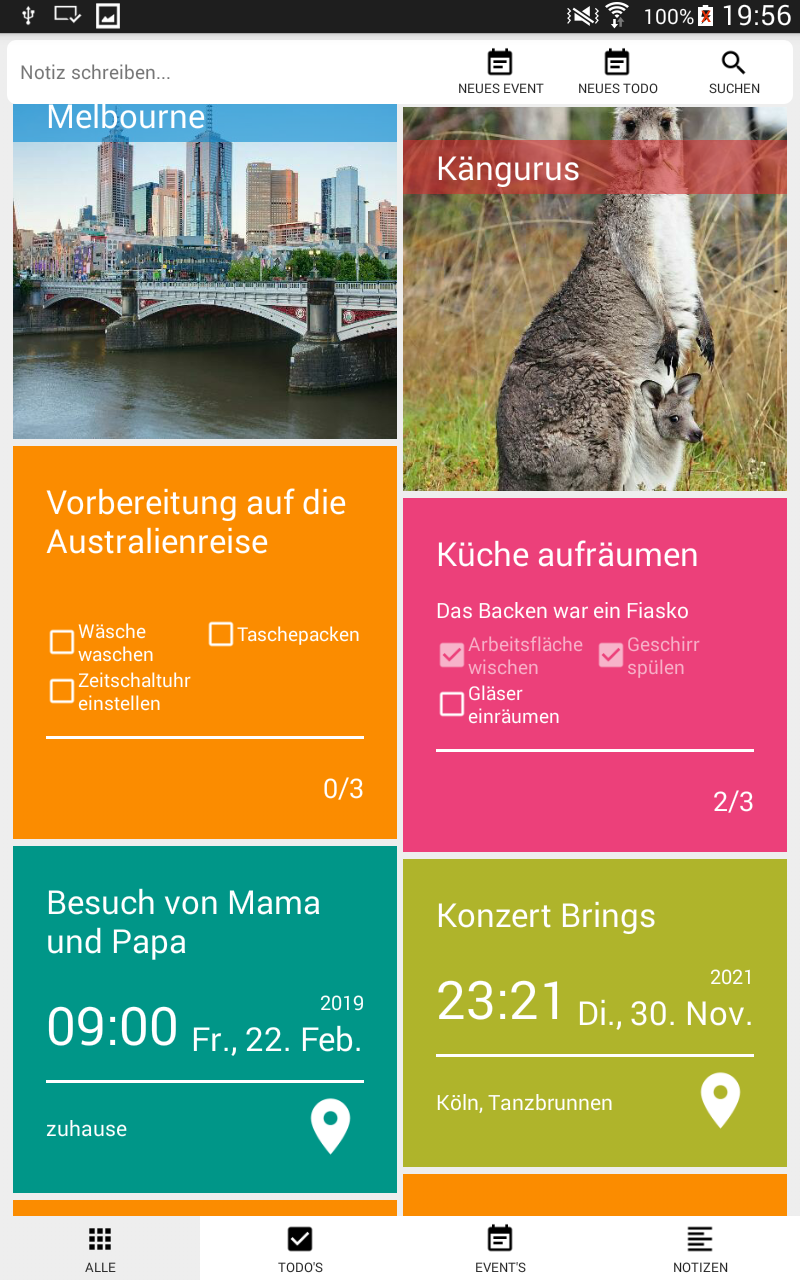
\includegraphics[width=1\textwidth]{img/Overview}\\ % Pfad
\source{Screenshot aus der Benutzeroberfläche} % Quelle
\end{minipage}
\end{figure}

Die Activity Overview zeigt normal 2 Spalten mit Fragments, wenn jedoch das Tablet gedreht wird zeigt die Landscape-Ansicht drei Spalten mit Fragments, um den Bildschirm optimal zu nutzen.

\begin{figure}[H]
\centering
\begin{minipage}[t]{1\textwidth} % Breite, z.B. 1\textwidth		
\caption{Landscape Ansicht - Overview Activity} % Überschrift
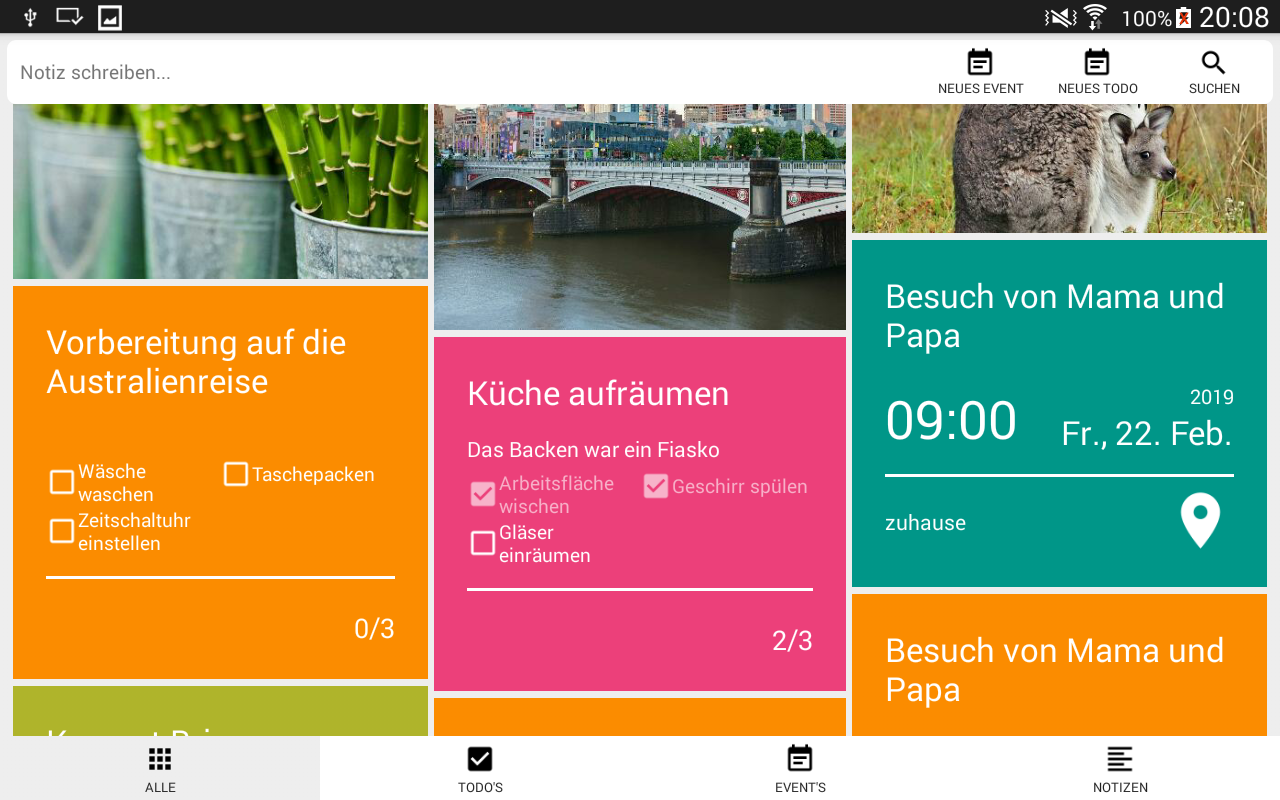
\includegraphics[width=1\textwidth]{img/Landscape}\\ % Pfad
\source{Screenshot aus der Benutzeroberfläche} % Quelle
\end{minipage}
\end{figure}

Die drei verschiedenen Arten von Fragments sind Notes, ToDo und Event.

Bei einer Note wird die Überschrift und ein Textauszug angezeigt. Wenn jedoch ein Bild in der Notiz vorhanden ist wird dieses mit der Überschrift in der Overview Activity angezeigt.

\begin{figure}[H]
\centering
\begin{minipage}[t]{1\textwidth} % Breite, z.B. 1\textwidth		
\caption{Note Fragments} % Überschrift
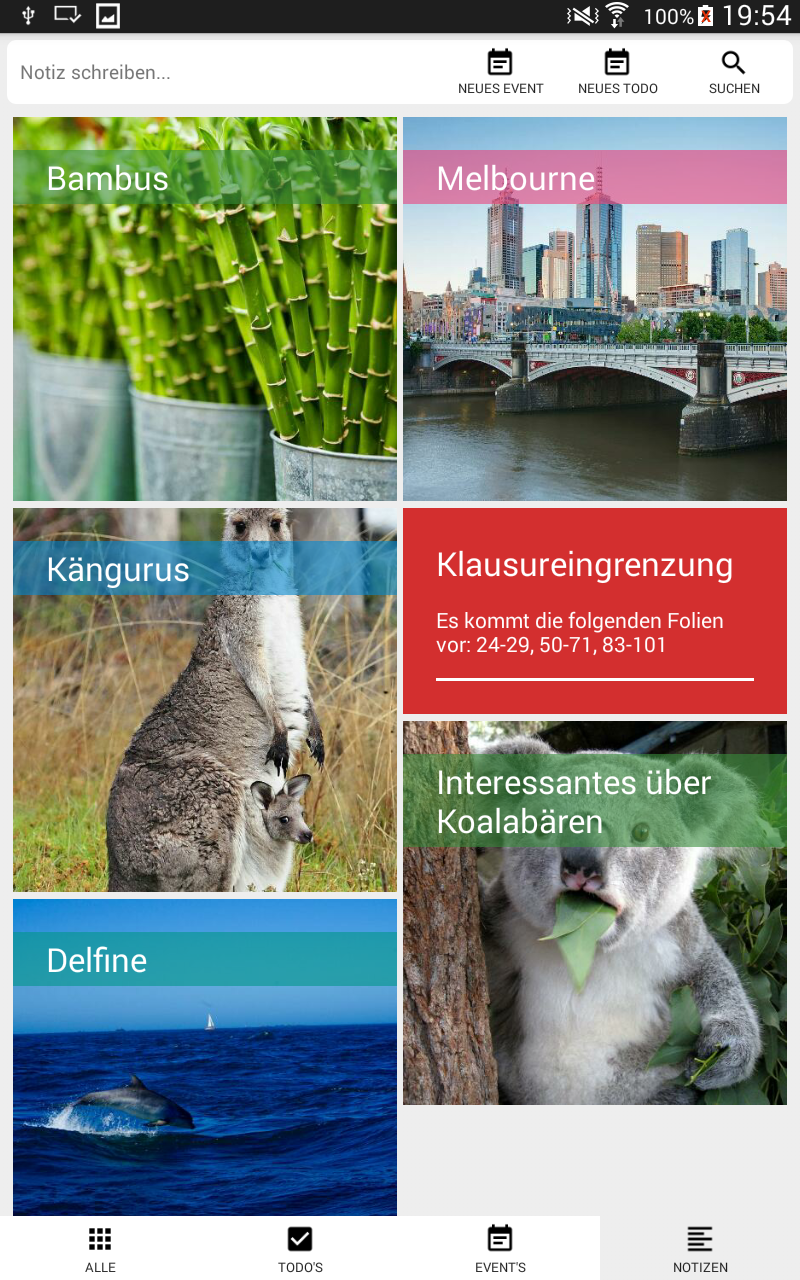
\includegraphics[width=1\textwidth]{img/FragmentN}\\ % Pfad
\source{Screenshot aus der Benutzeroberfläche} % Quelle
\end{minipage}
\end{figure}

Die Fragments für die ToDos, zeugen auch den Titel an und die einzelnen Aufgaben mit Kästchen, die mit einem Hacken gefüllt sind, wenn sie erledigt sind. Zusätzlich wird Angezeigt, wie viele Aufgaben schon erfüllt wurden.

\begin{figure}[H]
\centering
\begin{minipage}[t]{1\textwidth} % Breite, z.B. 1\textwidth		
\caption{Todo Fragments} % Überschrift
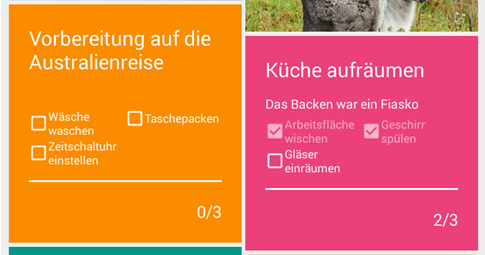
\includegraphics[width=1\textwidth]{img/FragmentT}\\ % Pfad
\source{Screenshot aus der Benutzeroberfläche} % Quelle
\end{minipage}
\end{figure}

Die Event Fragmentes bestehen aus der Überschrift, dem Datum und der Uhrzeit, sowie aus einem Ort, der angegeben werden kann.

\begin{figure}[H]
\centering
\begin{minipage}[t]{1\textwidth} % Breite, z.B. 1\textwidth		
\caption{Event Fragments} % Überschrift
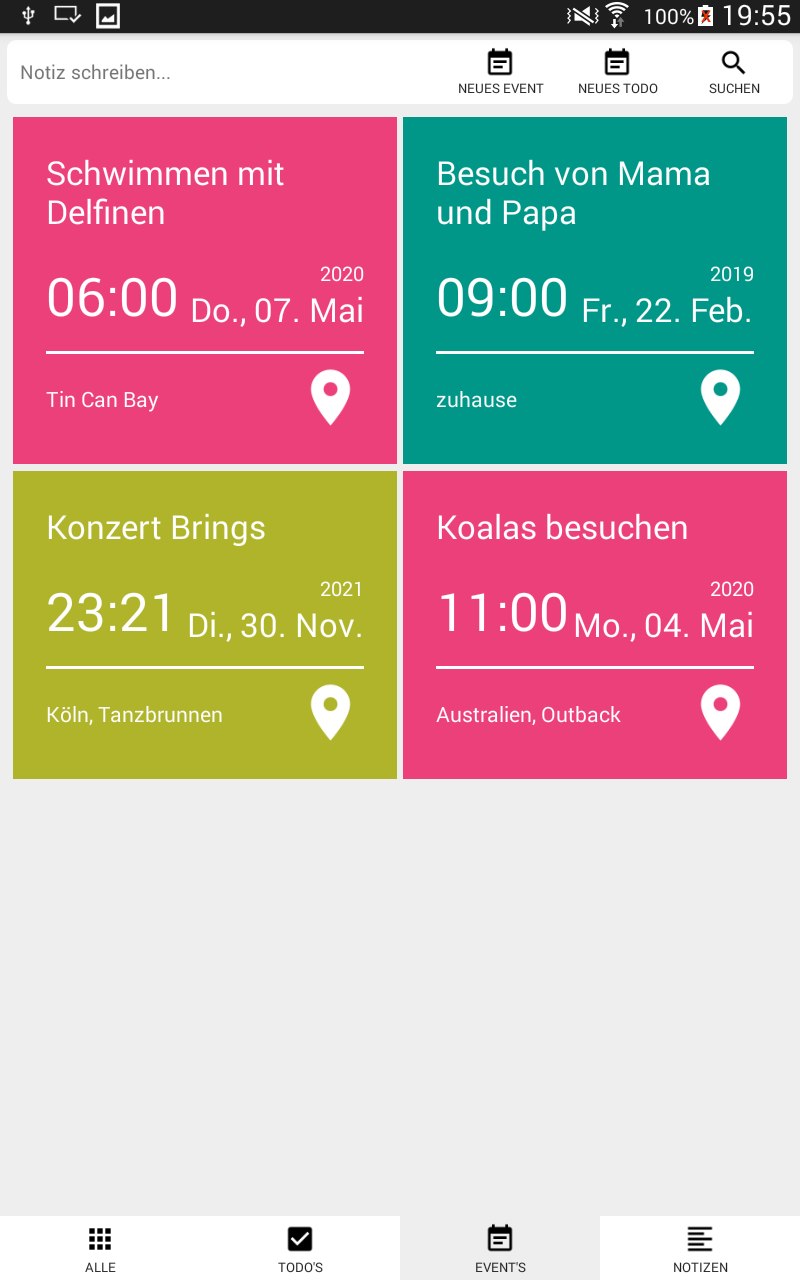
\includegraphics[width=1\textwidth]{img/FragmentE}\\ % Pfad
\source{Screenshot aus der Benutzeroberfläche} % Quelle
\end{minipage}
\end{figure}

In der Overview Activity kann zusätzlich gesucht und gelöscht werden. Wenn man einen langen Click auf ein Fragment macht, wird die obere Leiste verändert und man bekommt einen Button zum Löschen. Zusätzlich kann in dieser Ansicht nun auf die verschiedenen Fragments geklickt werden, um diese zu markieren und mehrere gleichzeitig zu löschen. Diese Ansicht kann durch den Zurück-Pfeil verlassen werden.

\begin{figure}[H]
\centering
\begin{minipage}[t]{1\textwidth} % Breite, z.B. 1\textwidth		
\caption{Overview Activity - Löschen} % Überschrift
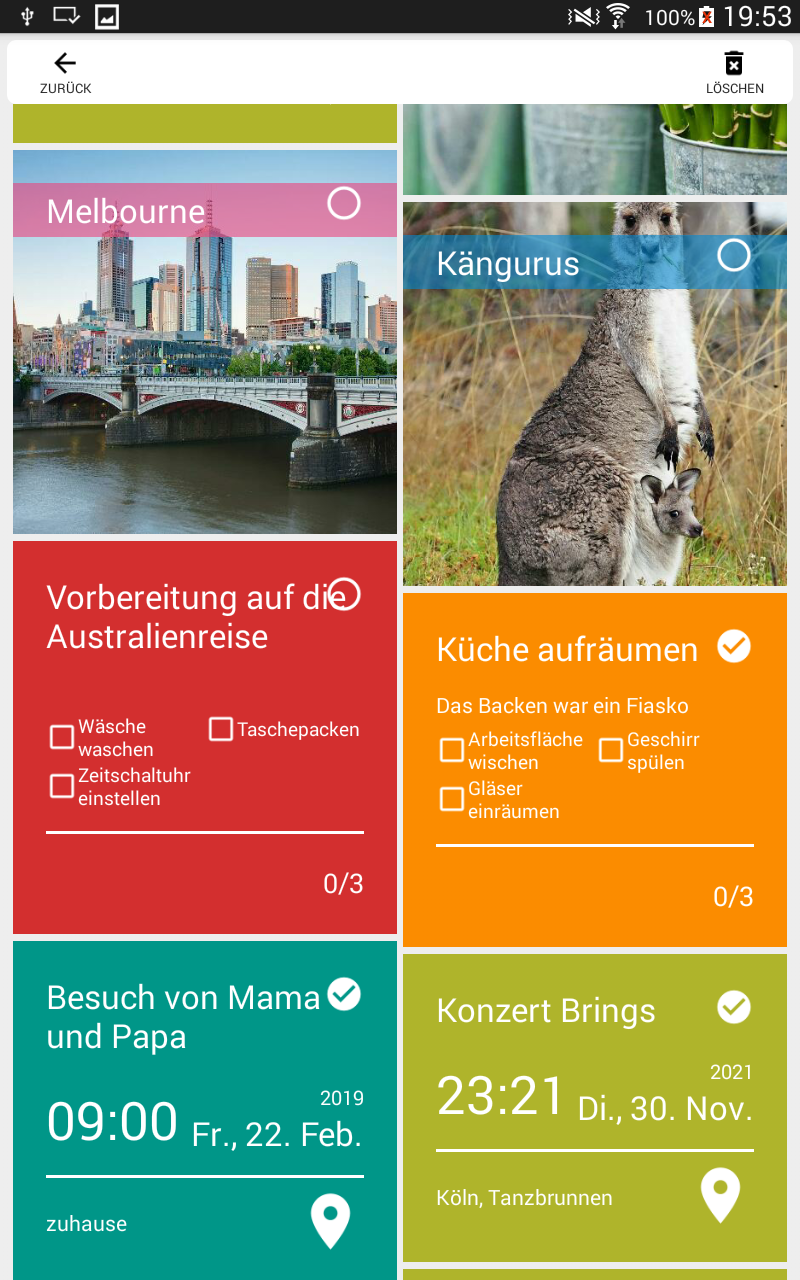
\includegraphics[width=1\textwidth]{img/Loeschen}\\ % Pfad
\source{Screenshot aus der Benutzeroberfläche} % Quelle
\end{minipage}
\end{figure}

Auch bei der Suchfunktion wird die obere Leiste angepasst. Dabei kann nun ein beliebiges Wort eingegeben werden, welches dann in den verschiedenen Einträgen gesucht wird. Die gefundenen Einträge werden daraufhin angezeigt. Um die Suche zu beenden kann der Zurück-Pfeil verwendet werden.

\begin{figure}[H]
\centering
\begin{minipage}[t]{1\textwidth} % Breite, z.B. 1\textwidth		
\caption{Overview Activity - Suchen} % Überschrift
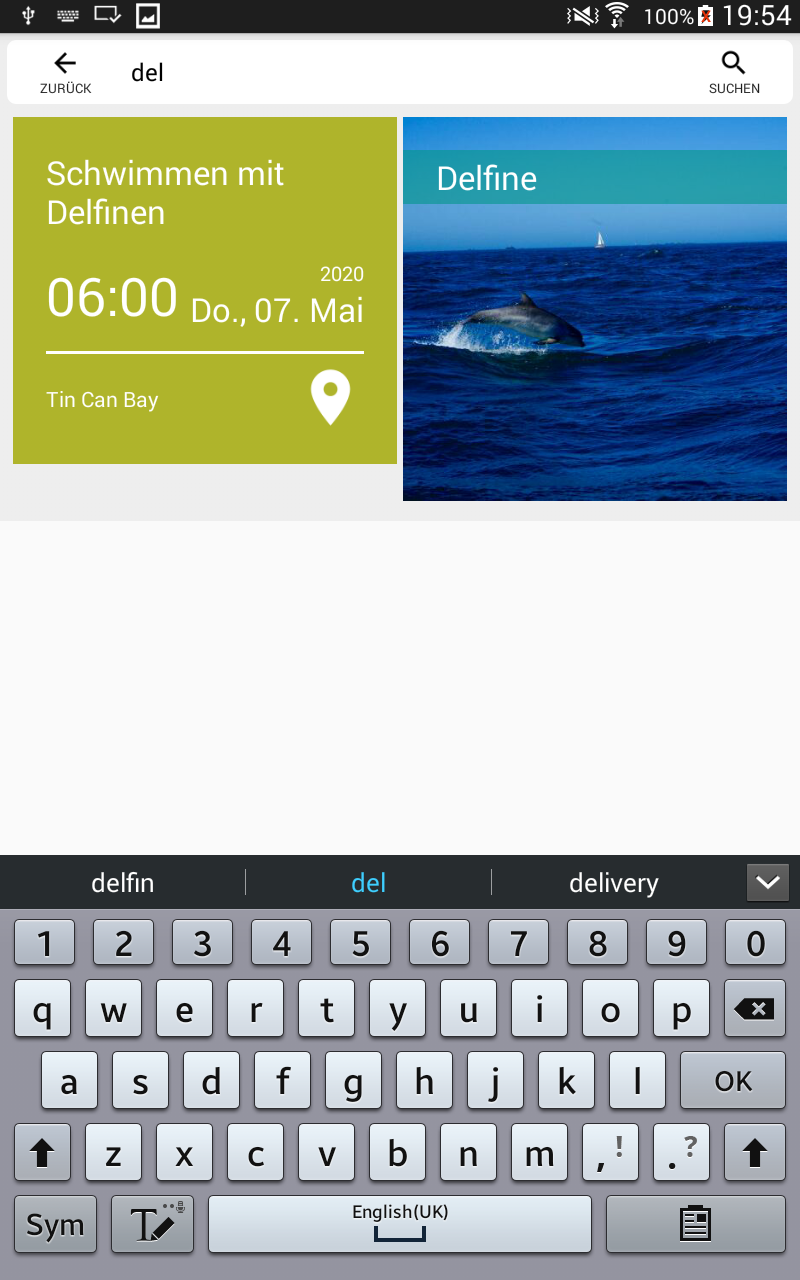
\includegraphics[width=1\textwidth]{img/Suchen}\\ % Pfad
\source{Screenshot aus der Benutzeroberfläche} % Quelle
\end{minipage}
\end{figure}

%Yannick
\textbf{Use Case (Yannick Rüttgers)}\\
Wie bereits geschrieben, dient diese Activity dem Nutzer als Einstiegspunkt in die Applikation. Hier kann er einige Aktionen durchführen.
 
Zum einen kann er die Oberfläche der Übersicht selbst beeinflussen. Hierzu gibt es am unteren Bildschirmrand einige Buttons, mit denen er nach den verschiedene TEN-Arten filtern kann. Zusätzlich kann er über eine Suchfunktion alle TENs durchsuchen.

Aus dieser Activity heraus können vom User auch neue TENs erstellt werden. Hierzu wird er allerdings an weitere Activities weitergeleitet.

Zuletzt ist es dem Nutzer auch möglich, mehrere TENs auf einmal zu löschen. Dies geschieht, wie bereits gesagt, über ein markieren einzelner Kacheln.

Im Folgenden ist das Usecase-Diagramm für die Übersicht zu sehen.

\begin{figure}[H]
\centering
\begin{minipage}[t]{1\textwidth} % Breite, z.B. 1\textwidth		
\caption{Usecase Diagramm der Overview} % Überschrift
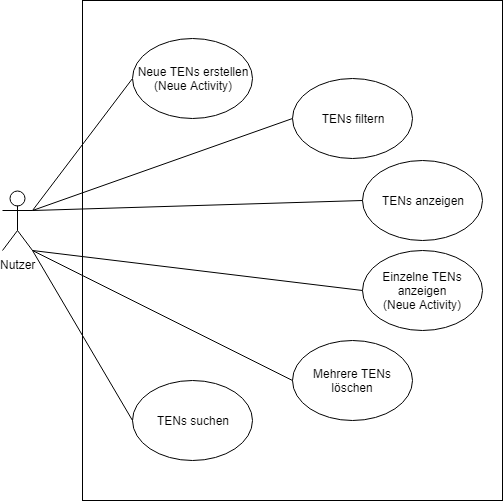
\includegraphics[width=1\textwidth]{img/Usecase_Overview}\\ % Pfad
\source{Erstellt von Yannick Rüttgers} % Quelle
\end{minipage}
\end{figure}

%Yannick
\textbf{Datenstruktur und Typen (Yannick Rüttgers)}\\
Die Daten für diese Activity werden hauptsächlich über die Klasse OverviewData verwaltet.

Wenn die Activity initiiert wird, werden zuerst alle nötigen Instanzen erstellt. Hierzu gehört unter anderen eine Instanz der Klasse OverviewData. Diese Klasse ruft in ihrem Konstruktor mithilfe einer statischen Servicemethode alle TENs als Objekte ab. Diese Objekte werden in einer ArrayList gespeichert. Bei Bedarf werden diese Daten neu geladen.

Um beim Suchen oder Filtern nicht alle Daten neu laden zu müssen, gibt es eine weitere ArrayList, die immer den gefilterten Datenstand enthält. Aus diesen Daten werden die Fragments generiert.

Um die Filterung von Fragments beim Wechsel der Orientierung der Applikation beibehalten zu können, wird dies ebenfalls im Dataobjekt hinterlegt.

Wenn Fragments generiert werden, bekommen diese die Daten des zugehörigen TEN-Objekts als Bundle mitgegeben. Während der Initialisierung jedes Fragments, werden die Daten im jeweiligen Data Objekt abgelegt. Die Parameter dieser Dataobjekte bilden zum größten Teil die der TEN-Objekte ab. Im Konstruktor der Dataklasse werden den einzelnen Parametern dann die Werte aus dem Bundle zugewiesen. Da in der Activity die TENs nicht bearbeitet werden können, gibt es im Nachhinein keine Möglichkeit den Fragments neue Daten zuzuweisen.

Zusätzlich hält jedes Fragment zwei Informationen über sich. Dies ist zum einen der Löschzustand, über den das Fragment steuern kann, ob es zum Löschen markiert werden kann oder nicht. Zum anderen hält das Fragment die Information, ob es markiert ist, um dies im Falle einer Löschung angeben zu können. Diese beiden Informationen können aus dem Fragment abgerufen werden.

%Yannick
\textbf{Dokumentation des Quelltextes der Activity (Yannick Rüttgers)}\\
Allgemein
Die OverviewActivity besteht aus 35 verschiedenen Klassen. Diese Klassen sind in verschiedene Pakete unterteilt.
Zum einen gibt es die Klassen, die unmittelbar zur OverviewActivity an sich gehören. Zu diesen zugehörig sind die Klassen, die für den Header der Activity genutzt werden.
Alle weiteren Klassen werden für die Fragments, die die TENs darstellen, genutzt. Hierzu gibt es vier Superklassen und zwei Listener, die in allen Fragments genutzt werden. Jedes der vier verschiedenen Fragments hat nochmal vier weitere Klassen, die von den Superklassen erben.
In Folgender Grafik soll dies verdeutlicht werden.
 
\begin{figure}[H]
\centering
\begin{minipage}[t]{1\textwidth} % Breite, z.B. 1\textwidth		
\caption{Klassendiagramm} % Überschrift
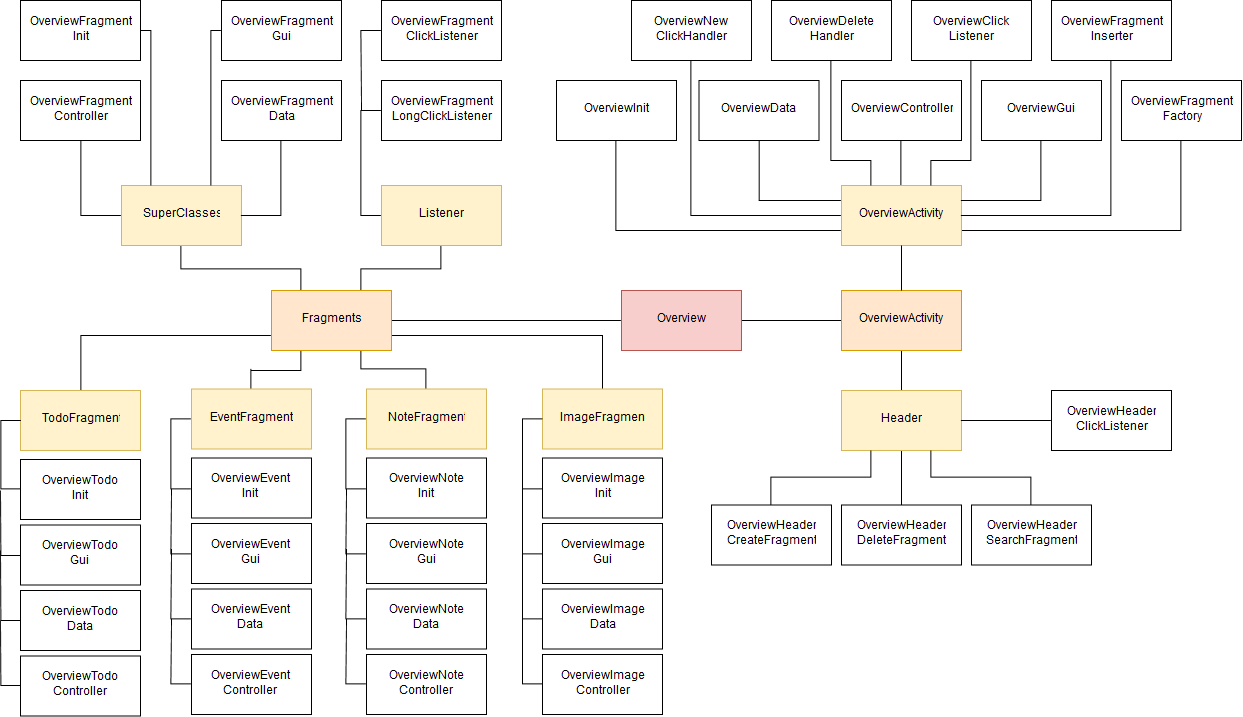
\includegraphics[width=1\textwidth]{img/Klassendiagramm_lite}\\ % Pfad
\source{Erstellt von Yannick Rüttgers} % Quelle
\end{minipage}
\end{figure}

Die Funktion der Klassen und wichtige Methoden werden im Folgenden erläutert.
Activityklassen
Zu den Klassen, die unmittelbar zur Activity gehören, zählen neun verschiedene Klassen.
Klasse: class OverviewInit extends AppCompatActivity
Diese Klasse ist für die Initialisierung der verschiedenen Komponenten der Activity zuständig. Da sie von der Superklasse AppCompatActivity erbt, implementiert sie zusätzlich die Methoden des Activitylifecycles.
Wichtige Methoden:
-protected void OnCreate(Bundle savedInstanceState)
Diese Methode ist eine der Lifecyclemethoden von Activities, sie wird beim entstehen der Activity aufgerufen. Hier werden die verschiedenen Komponenten der Activity mit den zugehörigen Methoden initiiert.
-public void onConfigurationChanged(Configuration newConfig)
Diese Methode wird aufgerufen, wenn sich etwas an der Konfiguration der Applikation ändert, wie in diesem Fall die Ausrichtung des Gerätes. Hier werden der Controller und die Gui neu initiiert. Dazu werden die Methoden initGui() und initController() aufgerufen.
Klasse: class OverviewData
Diese Klasse ist für die Datenhaltung innerhalb der Activity verantwortlich. Hier befinden sich auch die zum Sortieren und zum Suchen verwendeten Methoden. Initial werden die Daten einmal geladen, bei Bedarf werden diese über eine Methode neugeladen. Die Daten werden dabei zweimal gehalten: Eine Liste enthält alle TENs, die andere Liste enthält die TENs, die angezeigt werden sollen.
Wichtige Methoden:
-public void refresh()
Läd die Daten neu.
-public ArrayList<TEN> filterData()
Filtert die Daten nach dem aktuell ausgewählten TEN-Typen.
-public void search(String pSearchString)
Fügt nur die Suchergebnisse in die Liste der TENs ein, die angezeigt werden sollen.
Klasse: class OverviewGui
Diese Klasse verwaltet die Benutzeroberfläche der Activity.
Wichtige Methoden:
-public void markButton(Class pClass)
Markiert einen der Buttons am unteren Bildschirmrand, je nachdem welcher TEN-Typ ausgewählt ist.
-public void showFooter() / hideFooter()
Zeigt oder versteckt die Buttons am unteren Bildschirmrand.
Klasse: class OverviewController
Diese Klasse verwaltet die einzelnen Helferklassen und stellt die Logik der Activity da. 
Wichtige Methoden:
In der Klasse wird die Suche aktiviert, sowie das Löschen von TENs verwaltet. Hierzu werden die Helferklassen OverviewDeleteHandler, OverviewNewClickHandler, OverviewFragmentFactory und OverviewFragmentInserter genutzt. 
Klasse: class OverviewFragmentFactory
Diese Klasse erstellt verschiedene Arten von Fragments, die dann später genutzt werden können.
Wichtiger Methoden:
-public Fragment createHeader(Create/Delete/Search)Fragment()
Diese Methode liefert das gewählte Headerfragment zurück.
-public ArrayList<Fragment> createTENFragments(ArrayList<TEN> pTENs)
Erstellt eine Liste von Fragments, die aus den TENs erstellt werden. Je nach Art des TENs wird ein unterschiedliches Fragment erstellt.
Klasse: class OverviewFragmentInserter
Diese Klasse fügt Fragments in die Benutzeroberfläche ein. Hierzu wird der FragmentManager der Activity genutzt.
Wichtige Methoden:
-public void insertFragment(int pContainerID, Fragment pFragment, String pTag)
Fügt ein Fragment in einen gewählten Container ein. Dem Fragment wird ein Tag zugewiesen.
-public void replaceFragment(int pContainerID, Fragment pFragment, String pTag)
Ersetzt ein Fragment in einem gewählten Container durch ein anderes. Dem Fragment wird ein Tag zugewiesen.
-public void insertFragments(int[] pContainerIDs, ArrayList<Fragment pFragments)
Fügt eine beliebige Anzahl Fragments in eine beliebige Anzahl Container an. Dabei werden die Container zyklisch durchlaufen.
Klasse: class OverviewClickListener
Diese Klasse verwaltet die Klickevents der OverviewActivity. Je nach geklicktem Button wird eine andere Methode des Controllers aufgerufen.
Wichtige Methoden:
-public void onClick(View view)
Ruft je nach angeklickter View die show()-Methode des Controllers mit einem bestimmten Parameter auf.
Klasse: class OverviewDeleteHandler
Diese Klasse verwaltet die Methoden, die zum Löschen beziehungsweise nicht Löschen von TENs nötig sind.
Wichtige Methoden:
-public void longClick()
Aktiviert den Löschvorgang für alle Fragments.
-public void back()
Deaktiviert den Löschvorgang für alle Fragments.
-public void delete()
Sammelt alle markierten Fragments und löscht die dazugehörigen TENs. Deaktiviert den Löschvorgang für alle anderen Fragments.
Klasse: class OverviewNewClickHandler
Verwaltet das Erstellen von neuen TENs.
Wichtige Methoden:
-public void newTEN(Class pClass)
Startet eine neue Activity, je nachdem welche TEN-Art angegeben wurde.
Header
Die Header der Activity sind wechselnde Fragments, die verschiedene Aufgaben haben. Sie werden am oberen Bildschirmrand ausgetauscht. Ein Fragment dient dem Neuerstellen von TENs, eines das Löschen und eines das Suchen.
Die Fragments teilen sich einen ClickListener.
Klasse: class OverviewHeaderCreateFragment
Dieses Fragment dient dazu, das Erstellen von neuen TENs anzustoßen. Hierzu enthält es drei Buttons. Zusätzlich gibt es einen Button zum Starten der Suche.
Klasse: class OverviewHeaderDeleteFragment
Dieses Fragment dient dem Löschvorgang. Es gibt einen Button zum Abbrechen des Prozesses und einen Button, um die Löschung durchzuführen.
Klasse: class OverviewHeaderSearchFragment
Dieses Fragment dient dem Suchvorgang. Es gibt ein Textfeld, in das ein Suchbegriff eingegeben werden kann. Außerdem gibt es einen Button zum Abbrechen des Prozesses und einen, um die Suche durchzuführen.
Klasse: class OverviewHeaderClickListener
Diese Klasse behandelt die Clickevents der Headerfragments. Je nachdem, welcher Button in einem der Fragments geklickt wurde, wird eine andere Methode im Controller aufgerufen.
Wichtige Methoden:
-public void onClick(View view)
Diese Methode wird ausgeführt, sobald einer der Buttons eines Headers geklickt wird. Je nachdem, welcher Button dies war, wird eine Methode im Controller aufgerufen.
Superklassen
Die folgenden Klassen dienen als Superklassen für die Fragments. Dies wurde so entwickelt, da alle vier Fragments sich ähnliche Funktionen teilen. Große Teile der Implementierung nutzen außerdem die Polymorphie.
Klasse: class OverviewFragmentInit
Diese Klasse dient als Superklasse für die Initialklassen der einzelnen Fragments. Hier werden die anderen drei Komponenten der Fragments initialisiert. Ausserdem werden zum Start des Fragments mehrere andere Methoden aufgerufen.
Wichtige Methoden:
-public void onCreateView(Bundle pArguments, View pView)
Diese Methode startet, wenn das Fragment erstellt wird, verschiedene Methoden des Controllers.
Klasse: class OverviewFragmentData
Diese Klasse dient als Superklasse für die Dataklassen der einzelnen Fragments. Sie bildet die Klasse TEN nach.
Wichtige Methoden:
-public void addData(Bundle pData)
Diese Methode pflegt die Daten aus einem Bundle in das Objekt ein.
Klasse: class OverviewFragmentGui
Diese Klasse dient als Superklasse für die Guiklassen der einzelnen Fragments. Sie kümmert sich um den Markierungsprozess der Fragments für den Löschvorgang.
Wichtige Methoden:
-public void applyMarked(boolean pMarked)
Diese Methode setzt den Zustand des Checkboxicons auf den des übergebenen Zustandes.
Klasse: class OverviewFragmentController
Diese Klasse dient als Superklasse für die Controllerklassen der einzelnen Fragments. Hauptsächlich wird sich auch hier um den Löschprozess gekümmert, da dieser für alle Fragments gleich ist.
Wichtige Methoden:
-public void longClicked()
Diese Methode startet den Löschprozess. Dazu wird der Controller der Activity, die das Fragment verwaltet aufgerufen, und ihm mitgeteilt, dass der Löschprozess gestartet werden soll.
Listener
Klasse: class OverviewFragmentClickListener
Diese Klasse ist dafür zuständig, dass, wenn ein Fragment angeklickt wird, im Controller dieses Fragments eine Methode ausgeführt wird. So wird eines der Fragments geöffnet.
Klasse: class OverviewFragmentLongclickListenerFragment
Diese Klasse ist dafür zuständig, dass, wenn ein Fragment lange angeklickt wird, die entsprechende Methode im Controller des Fragments aufgerufen wird. So gelangt der Nutzer in den Löschvorgang.
Fragments
Die folgenden Kapitel behandeln die vier genutzten Fragments. Alle Fragments erben von den vier zuvor genannten Superklassen, und teilen sich so eine Struktur. Zudem wird, um den Quellcode übersichtlich zu halten, viel Wert auf die Nutzung von Polymorphie gelegt.
TodoFragment
Die folgenden Klassen implementieren das Fragment, welches die Todos abbildet.
Klasse: class OverviewTodoInit
Diese Klasse initiiert alle nötigen Komponenten für das Todo-Fragment.
Klasse: class OverviewTodoData
Diese Klasse stellt die Datenhaltung für das Todo-Fragment dar. Sie bildet die Klasse Todo nach.
Wichtige Methoden:
-public void addData(Bundle pData)
Diese Methode pflegt die Daten aus einem Bundle in das Objekt ein.
Klasse: class OverviewTodoGui
Diese Klasse verwaltet die GUI für das Todo-Fragment. Hier geschieht auch die Generierung der Checkboxen aus den Todo-Tasks.
Wichtige Methoden:
-public void addView(View pView)
Diese Methode fügt die View des Fragments dem Objekt hinzu. Außerdem werden den Attributen Views zugewiesen.
-public void addCheckbox(boolean pStatus, String pDescription)
Fügt dem Fragment eine Checkbox hinzu, die aus einem Kästchen und einer Beschreibung besteht.
Klasse: class OverviewTodoController
Diese Klasse stellt die Logik des Todofragments dar. Hier werden den Feldern der Benutzeroberfläche Werte zugewiesen. Zusätzlich werden aus den Tasks des Todos Checkboxen generiert.
-public void applyData()
Diese Methode übergibt die Attribute des Dataobjekts an das Guiobjekt, damit die Views aktualisiert werden können.
-public void generateCheckboxes()
Diese Methode generiert aus der Taskliste des Todos mithilfe der addCheckbox-Methode des Guiobjekts Checkboxen.
EventFragment
Die folgenden Klassen implementieren das Fragment, welches die Events abbildet.
Klasse: class OverviewEventInit
Diese Klasse initiiert alle nötigen Komponenten für das Event-Fragment.
Klasse: class OverviewEventData
Diese Klasse stellt die Datenhaltung für das Event-Fragment dar. Sie bildet die Klasse Event nach. Hier wird das Kalenderobjekt in seine Einzelteile zerlegt.
Wichtige Methoden:
-public void addData(Bundle pData)
Diese Methode pflegt die Daten aus einem Bundle in das Objekt ein.
Klasse: class OverviewEventGui
Diese Klasse verwaltet die GUI für das Event-Fragment.
Wichtige Methoden:
-public void addView(View pView)
Diese Methode fügt die View des Fragments dem Objekt hinzu. Außerdem werden den Attributen Views zugewiesen.
Klasse: class OverviewEventController
Diese Klasse stellt die Logik des Eventfragments dar. Hier werden den Feldern der Benutzeroberfläche Werte zugewiesen.
-public void applyData()
Diese Methode übergibt die Attribute des Dataobjekts an das Guiobjekt, damit die Views aktualisiert werden können.
NoteFragment
Die folgenden Klassen implementieren das Fragment, welches die Notes abbildet, die keine Bilder haben.
Klasse: class OverviewNoteInit
Diese Klasse initiiert alle nötigen Komponenten für das Note-Fragment.
Klasse: class OverviewNoteData
Diese Klasse stellt die Datenhaltung für das Note-Fragment dar. Sie bildet die Klasse Note nach.
Wichtige Methoden:
-public void addData(Bundle pData)
Diese Methode pflegt die Daten aus einem Bundle in das Objekt ein.
Klasse: class OverviewNoteGui
Diese Klasse verwaltet die GUI für das Note-Fragment.
Wichtige Methoden:
-public void addView(View pView)
Diese Methode fügt die View des Fragments dem Objekt hinzu. Außerdem werden den Attributen Views zugewiesen.
Klasse: class OverviewNoteController
Diese Klasse stellt die Logik des Note-Fragments dar. Hier werden den Feldern der Benutzeroberfläche Werte zugewiesen.
-public void applyData()
Diese Methode übergibt die Attribute des Dataobjekts an das Guiobjekt, damit die Views aktualisiert werden können.
ImageFragment
Die folgenden Klassen implementieren das Fragment, welches die Notes abbildet, in denen Bilder gespeichert wurden.
Klasse: class OverviewImageInit
Diese Klasse initiiert alle nötigen Komponenten für das Image-Fragment.
Klasse: class OverviewImageData
Diese Klasse stellt die Datenhaltung für das Image-Fragment dar. Hier wird das Previewimage für die Notiz geladen.
Wichtige Methoden:
-public void addData(Bundle pData)
Diese Methode pflegt die Daten aus einem Bundle in das Objekt ein und läd das Previewimage.
Klasse: class OverviewImageGui
Diese Klasse verwaltet die GUI für das Image-Fragment.
Wichtige Methoden:
-public void addView(View pView)
Diese Methode fügt die View des Fragments dem Objekt hinzu. Außerdem werden den Attributen Views zugewiesen.
Klasse: class OverviewImageController
Diese Klasse stellt die Logik des Image-Fragments dar. Hier werden den Feldern der Benutzeroberfläche Werte zugewiesen.
-public void applyData()
Diese Methode übergibt die Attribute des Dataobjekts an das Guiobjekt, damit die Views aktualisiert werden können.

\subsubsection{Todo Activity}
%Florian
\textbf{Aufgabe und Funktionen (Florian Rath)}\\
Die Activity Todo dient dem Nutzer dazu, seine Aufgaben zu organisieren. Wenn er eine neue Todo erstellt hat, hat er die Möglichkeit einen Titel und eine Beschreibung einzugeben. Diese Eingabemöglichkeiten sind jedoch optional und hindern den Nutzer nicht daran, die Todo wieder zu verlassen und somit abzuspeichern. Der Titel für eine Todo könnte beispielsweise „Einkaufsliste“ lauten, während die Beschreibung nähere Informationen wie zum Beispiel „Für die Geburtstagsparty von meiner Tochter“ beinhalten kann. So hat der Benutzer die Möglichkeit mehrere Einkaufslisten anzulegen und sie mit einer Beschreibung voneinander differenzieren.

Neben dem Titel und der Beschreibung können auch ein Start- und Enddatum festgelegt werden. Dies ist hilfreich, wenn für eine Todo bestimmte Fristen vorhanden sind. Geht es in der Todo z.B. um eine Prüfungsvorbereitung, kann der Benutzer auswählen, wann er spätestens mit dem Lernen anfangen muss und bis wann er spätestens mit dem Lernen Zeit hat. Diese Funktionalität ist ebenfalls optional. Man kann also auch Todos verwenden, ohne ein bestimmtes Start- und Enddatum anzugeben. Die App zeigt dann immer jeweils das aktuelle Datum in den Eingabefeldern an.

Die Hauptfunktionalität der Todo-Activity ist das Anlegen von sogenannten Tasks.- Eine Task besteht im Prinzip aus einem Text, wie z.B. „Luftballons“, und einem Status (boolean-Wert). Der Status gibt an, ob ein Task erledigt ist oder nicht. Dies geschieht über eine Checkbox, die neben jedem Task vorhanden ist.

Unterstrichen wird die Gesamtfunktionalität mit einer Fortschrittsanzeige. Ein prozentualer Wert gibt dabei an, wie viele Tasks als erledigt markiert sind. Wurden z.B. 5 von 10 Tasks als erledigt markiert, steht in der App 50 Prozent. Sind es hingegen 1 von 10 markierte, dann nur noch 10 Prozent. Diese Funktionalität dient dazu, dem Benutzer einen Fortschritt über seine Todo zu geben. Anhand des Fortschritts kann er sich nämlich organisieren, ob er in den genannten Fristen liegt. Liegt man kurz wenige Tage vor einer Prüfung gerade bei 10 Prozent, so könnte es langsam brenzlig für den Benutzer werden. Auch in einer sehr langen Liste von Tasks könnte dieser Wert nützlich sein. Da die Todo-Activity darauf ausgelegt ist, theoretisch endlos viele Tasks speichern zu können (so viele, wie ein ArrayList speichern kann), können sehr lange Listen entstehen. Unter hunderten von Tasks könnte es schnell passieren, eine unerledigte Aufgabe zu übersehen und die Todo verfrüht abzuschließen. Die App macht keine Obergrenze für Tasks, um dem User keine Arbeits- bzw. Organisationsweise vorzuschreiben.

Der User hat auch die Möglichkeit eine Todo zu löschen.

%Sertan
\textbf{Layout, Screenshots (Sertan Cetin)}\\
Um eine maximale Bedienbarkeit zu gewährleisten, verfügt diese Activity insgesamt genau über zwei Layouts. Während das eine Layout die Benutzersteuerelement im Porträtmodus darstellt, dient das andere Layout dazu, die Elemente im Landscape-Modus darzustellen. Der Unterschied zwischen den beiden Layouts liegt in der Anordnung der Elemente. Im Porträtmodus belegt jedes Element eine Zeile auf dem Bildschirm. Sie sind also untereinander angeordnet. Im Landscape-Modus ist die Ansicht in zwei Spalten geteilt. In der linken Spalte sind der Titel, Beschreibung, Start- und Enddatum untereinander angeordnet. In der rechten Spalte befinden sich die einzelnen Aufgaben. Die Breite der linken Spalte hat einen festen Wert, nämlich 640px. Die Prozentanzeige befindet sich unabhängig von den beiden Spalten immer mittig am unteren Bildschirmrand.

Oben ist eine Toolbar vorhanden, mit einem Zurück-Button, um zur Hauptübersicht zu gelangen, und einem Menü, in welchem die Todo gelöscht werden kann.

Nachfolgender Screenshot zeigt den zuvor beschriebenen Landscape-Modus der Todo-Activity: 

\begin{figure}[H]
\centering
\begin{minipage}[t]{1\textwidth} % Breite, z.B. 1\textwidth		
\caption{Todo Activity im Landscape-Modus} % Überschrift
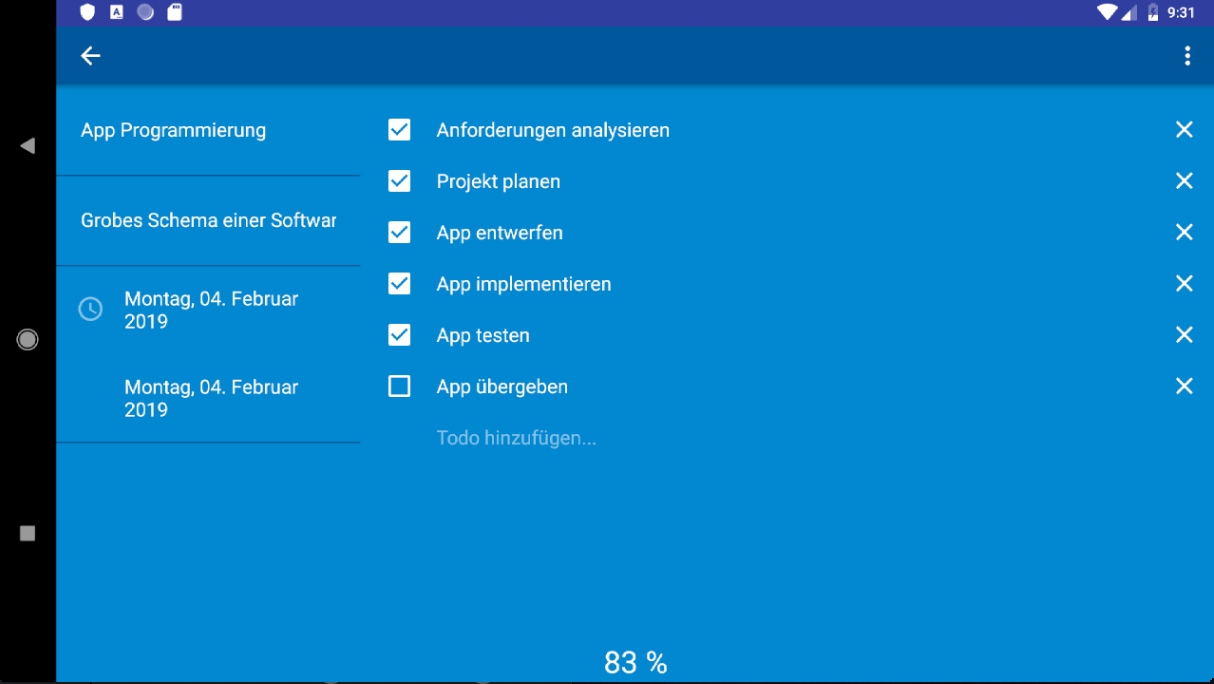
\includegraphics[width=1\textwidth]{img/Todo_landscape}\\ % Pfad
\source{Screenshot aus der Benutzeroberfläche} % Quelle
\end{minipage}
\end{figure}

Beim Wechsel der beiden Ansicht-Modi werden die Daten jeweils in das andere Layout übernommen.

\begin{figure}[H]
\centering
\begin{minipage}[t]{1\textwidth} % Breite, z.B. 1\textwidth		
\caption{Todo Activity im Portrait-Modus} % Überschrift
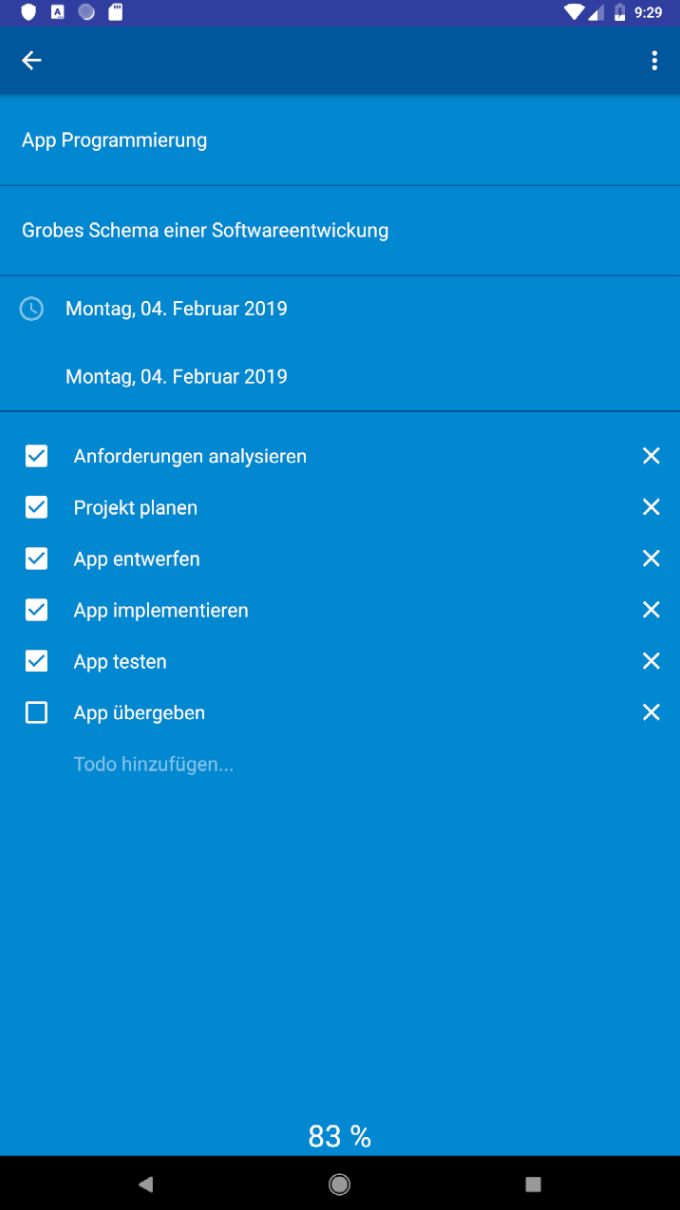
\includegraphics[width=1\textwidth]{img/Todo_portrait}\\ % Pfad
\source{Screenshot aus der Benutzeroberfläche} % Quelle
\end{minipage}
\end{figure}

Nachdem auf eines der Eingabefelder für Daten getippt wurde, initialisiert die Activity einen Datepicker und zeigt dem Benutzer ein gewohntes Auswahlmenü für ein gewünschtes Datum an. Dies hat den Vorteil, dass der Benutzer durch Erfahrungen in anderen Apps schnell und einfach mit der Datumeingabe zurechtfindet. Wie im Screenshot zu sehen ist, kann der Benutzer mit „Abbrechen“ die Datumsauswahl abbrechen, sodass das Eingabefenster geschlossen wird. Mit dem „Ok“-Button hat der Benutzer alternativ die Möglichkeit, seine Eingabe zu übernehmen. Hierbei liest die Activity das eingegeben Datum aus und stellt es formatiert dar. Es wird außerdem indem Todo-Objekt zwischengespeichert.

\begin{figure}[H]
\centering
\begin{minipage}[t]{1\textwidth} % Breite, z.B. 1\textwidth		
\caption{Datumeingabe} % Überschrift
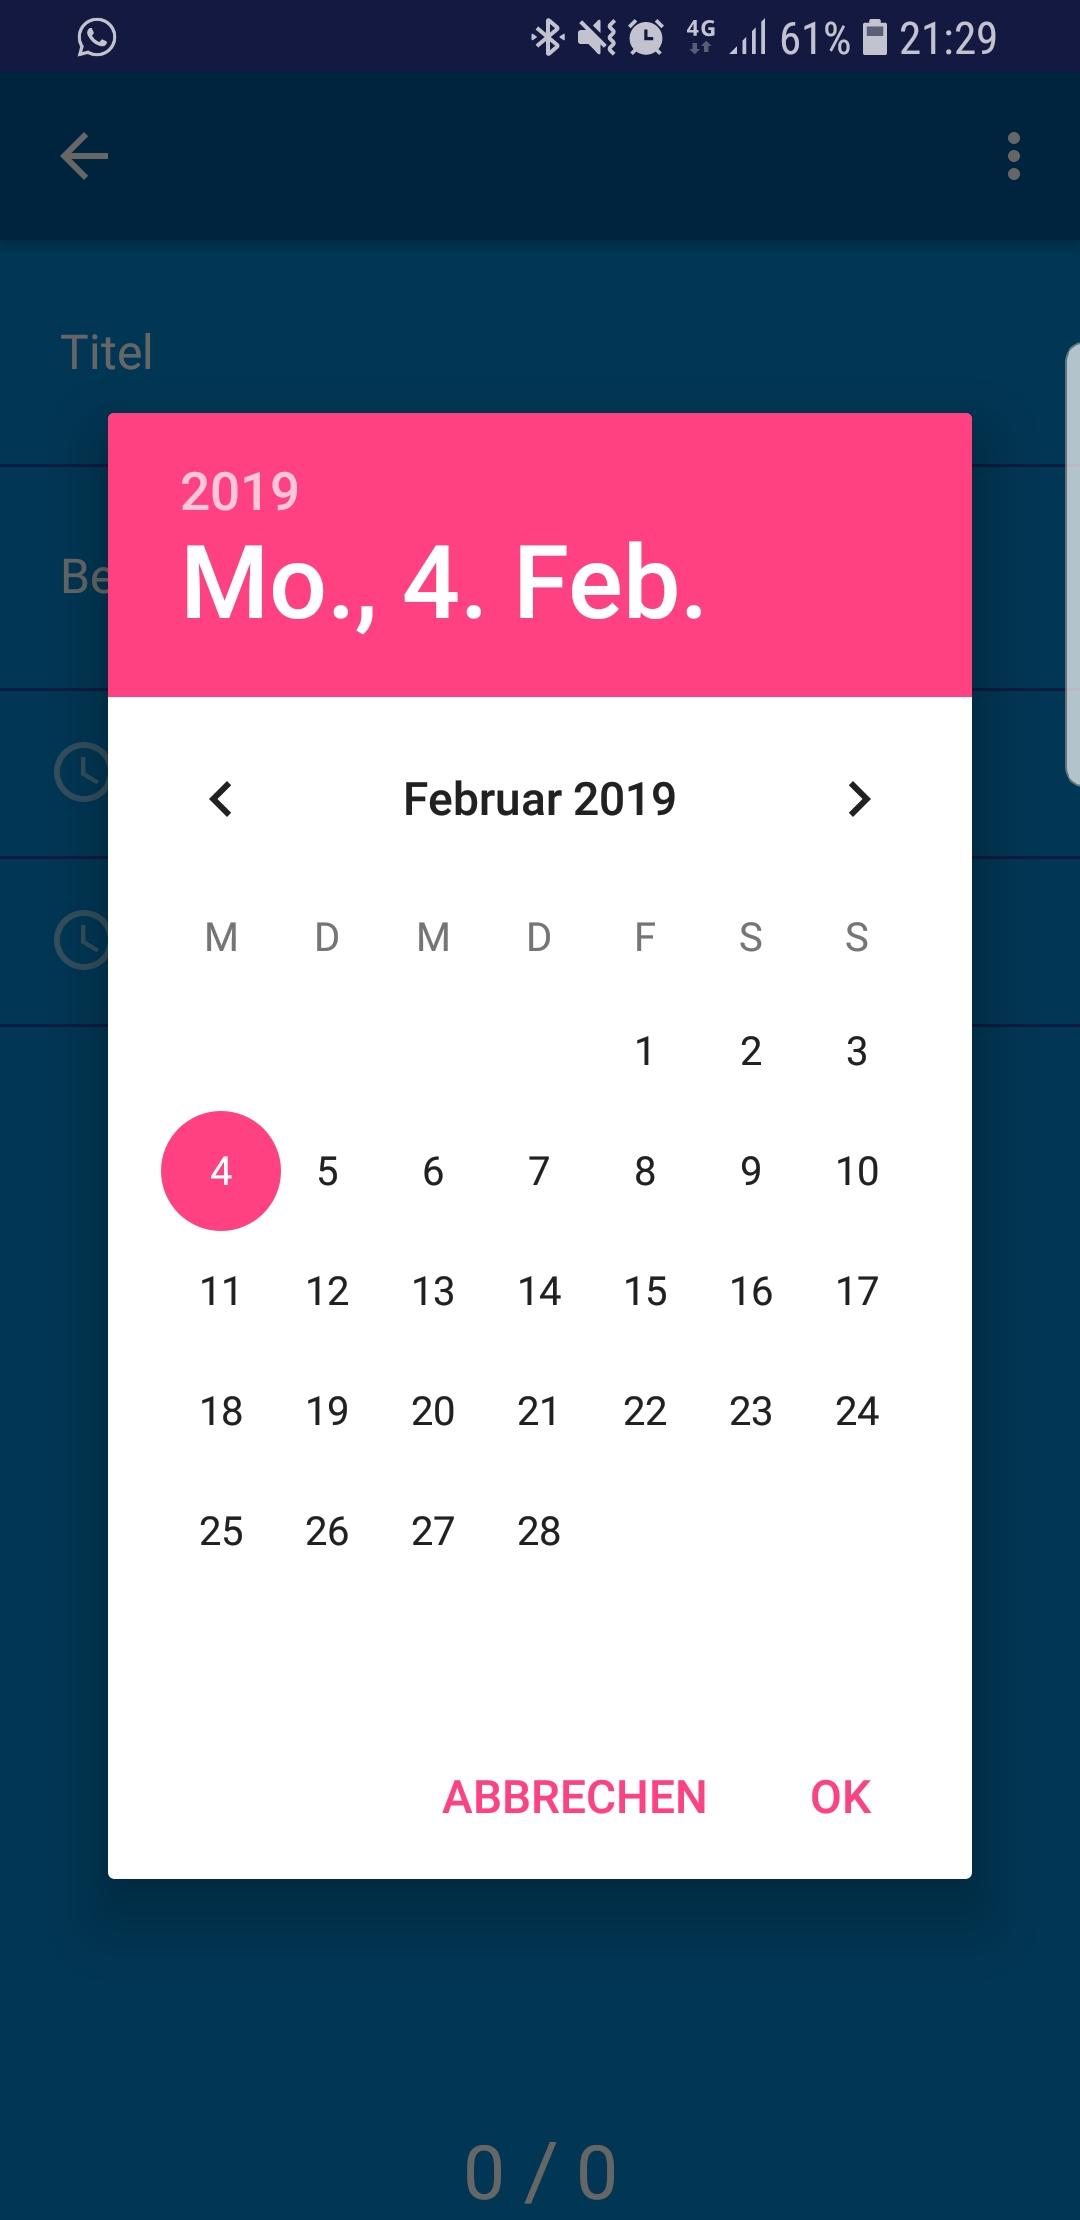
\includegraphics[width=1\textwidth]{img/Todo_Datepicker}\\ % Pfad
\source{Screenshot aus der Benutzeroberfläche} % Quelle
\end{minipage}
\end{figure}

%Florian
\textbf{Use Case (Florian Rath)}\\
Die Todo-Activity kann man über zwei Wege erreichen. Beide Wege erfolgen aus der Übersichts-Activity.

Der User kann entweder eine neue Todo erstellen, sodass in der Todo-Activity eine nicht vorhandene Todo-ID übergeben wird, oder er kann auf eine bereits vorhandene Todo tippen. Die ID dieser Todo wird dann aus der Datenbank geladen und in der Activity dargestellt. Die Todo-Activity deckt die Funktionalitäten des Todo-TEN‘s ab.

%Sertan
\textbf{Datenstrukturen und -typen (Sertan Cetin)}\\
Um die gewünschten Anforderungen zu erfüllen und dabei sowohl eine hohe Wartbarkeit als auch Modularität zu gewährleisten, wurden innerhalb der Todo-Activity mehrere Klassen implementiert. Nachfolgend werden diese Klassen vorgestellt.

Wenn die Todo-Activity aus der Overview-Activity gestartet wird, wird eine Instanz der Klasse Init, die die Schnittstelle AppCompatActivity implementiert, erstellt. In dieser Klasse werden weitere Klassen, die im Rahmen des Projektes angelegt wurden, erstellt. Bei diesen Klassen handelt es sich um Gui, TodoApplicationLogic und Data. Auf diese wird im Nachfolgenden näher eingegangen.

Die Gui-Klasse ist die Schnittstelle zum Layout. Hier werden alle Layout-Elemente in Variablen bzw. typgleichen Objekten gespeichert. So wird z.B. das Eingabefeld für den Titel in einer Variablen vom Datentyp EditText gespeichert. Indem jedes Element aus dem Layout in einer Variablen hinterlegt wird, erhält man die Möglichkeit diese vom Java-Code aus auszulesen bzw. zu manipulieren. Diese Klasse besitzt einen Konstruktor, in welchem die eigentliche Erstellung der genannten Objekte geschieht. Über Getter- und Setter-Methoden stellt die Gui-Klasse den anderen Klassen die Schnittstelle zum Layout zur Verfügung.

Die Data-Klasse speichert das Todo und stellt die Schnittstelle zwischen der Datenbank und der Applikationslogik dar. Sie ist somit für das Speichern, Löschen und Ändern verantwortlich. Im Konstruktor dieser Klasse wird außerdem das Todo-Objekt initialisiert. Beim Initialisierungsvorgang der Data-Klasse wird eine ID übergeben. Ist diese ID nicht vorhanden, wird legt sie ein neues Todo in der Datenbank an. Andernfalls wird das Todo geladen.

In der TodoApplicationLogic-Klasse findet die gesamte Geschäftslogik statt. Sie verbindet im Wesentlich die Data mit der Gui. Sie ist unteranderem für die Interaktion zuständig.

\textbf{Dokumentation des Quelltextes der Activity}\\
In diesem Kapitel wird der Quelltext der Todo-Activity vorgestellt und erläutert. Dabei wird Klasse für Klasse, Methode für Methode vorgegangen. 
Methoden der Init-Klasse (Sertan Soner Cetin)
Die Init Klasse verfügt insgesamt über 10 Methoden. Da die Klasse die Schnittstelle AppCompatActivity implementiert, sind die Methoden onCreate, onCreateOptionsMenu, onSaveInstanceState, onActivityResult, onBackPress und onConfigurationChanged vorhanden. Daneben sind noch Methoden wie initData, initGUI und initApplicationLogic vorhanden.
Private void initApplication() 
Diese Methode initialisiert das Objekt des Typs TodoApplicationLogic. Diese ApplicationLogic erhält die GUI- und Data-Objekte
Private void initData(String todoId)
Diese Methode initialisiert das Data-Objekt des Datentyps Data. Das Objekt erhält eine Instanz zur Activity und eine Todo-ID vom Typ String, welche dieser Methode ebenfalls übergeben wird.
Private void initGui()
Diese Methode initialisiert das Gui-Objekt. Dieses Objekt erhält eine Instanz zu der Activity.
Public void onCreate(Bundle savedInstanceState)
Diese Methode wird beim Erstellvorgang der Init-Klasse aufgerufen. Sie ruft die zuvor beschriebenen Methoden auf. Der Parameter savedInstanceState wird der Oberklasse übergeben.
Methoden der Gui-Klasse (Sertan Soner Cetin)
Die Gui-Klasse verfügt über einen Konstruktor, der im vorangegangenen Kapitel beschrieben wurde. Außerdem verfügt sie über diverse Getter- und Setter-Methoden. Es werden einige exemplarisch dargestellt.
Public void setFocusableInTouchmode(boolean value)
Diese Methode stellt den TouchModus des Layouts aus. Über den Parameter value kann angegeben werden, ob sich die Tastatur beim Start des Layouts aufklappen soll oder nicht. (true für nicht ausklappen, false für ausklappen)
Public EditText getmTitle()
	Diese Getter-Methode liefert das Objekt mTitle des Datentyps EditText zurück.
Public void setmTitle(string pTitle)
Diese Setter-Methode schreibt in das Textfeld des Todo-Layouts den übergebenen Parameter mit dem Namen pTitle des Datentyps String.
Public EditText getmText()
Diese Getter-Methode liefert das Objekt mText des Datentyps EditText zurück. Das Objekt entspricht dem Layout-Element für die Beschreibung des Todos.
Public void setColor(int color, int darkColor)
An diese Methode werden zwei Farbwerte als Integer übergeben. Der erste Farbwert entspricht einem helleren Farbton, z.B. Hellblau. Der zweite wäre ein dunklerer Blauton, z.B. Dunkelblau. Das Layout bekommt die helle Farbe als Hintergrundfarbe, während die Toolbar oder Trennlinien zwischen den einzelnen Elementen die dunklere Farbe erhalten.
Methoden der Data-Klasse (Sertan Soner Cetin)
Diese Klasse verfügt über einen Konstruktor und über Getter- und Setter-Methoden. Durch die Schnittstelle zur Datenbank sind noch Methoden für das Löschen und Ändern der Todo in der Datenbank vorhanden.
Public void deleteTodo()
	Löscht die Todo aus der Datenbank anhand seiner ID.
Public void updateTodo()
	Ändert die Todo in der Datenbank und aktualisiert somit alle Eigenschaften.
Public void setTitle(string title)
Ändert den Titel der Todo. Der Parameter title des Datentyps String ist der neue Titel.
Public boolean getmIsNew()
Gibt an, ob die Todo neuerstellt wurde oder beim Start der Activity bereits vorhanden war. Dieser Wert wird außerhalb benötigt, um festzulegen, ob sich die Tastatur beim Activity-Start aufklappen soll oder nicht.
Methoden der TodoApplicationLogic (Florian Rath)
Die TodoApplicationLogic stellt die größte Klasse innerhalb der Todo-Activity dar. Dies liegt unter anderem daran, dass die meisten Verantwortlichkeiten hier liegen. Sie ist Dreh und Angelpunkt der gesamten Infrastruktur, da sie die Data bzw. Datenbank mit der Gui bzw. dem Layout verbindet und alles steuert.
Private void initGui()
Diese Methode stellt die Gui ein und ruft eine andere Methode namens dataToGui auf.
Private void dataToGui()
Diese Methode schreibt die Todo-Eigenschaften auf die einzelnen Layout-Elemente. So wird z.B. der Todo-Titel in das Eingabefeld für den Titel geschrieben oder die Farbe des Todos als Hintergrundfarbe festgelegt.
Private void initListener()
Da innerhalb der Applikationslogik die Listener für die einzelnen Events z.B. ClickEvent oder TouchEvent verwaltet werden, wurde diese Methode angelegt, um alle Listener an einer zentralen Stelle zu initialisieren. Hier werden der ClickListener, TouchListener und CheckedChangeListener initialisiert und bei den einzelnen Layout-Elementen registriert.
Public void receiveDate(Date date)
Diese Methode wurde für den Datepicker benötigt. Sie empfängt quasi das Datum aus dem Eingabefeld. Der Parameter date wird dann an das Eingabefeld übergeben.
Public String formatDate(Date date)
Diese Methode liefert einen String zurück. Der Parameter date wird in eine leserliche Formatierung gebracht. Die Formatierung des Datums ist z.B. „Dienstag, 13. Januar 2019“.
Public void showDatePickerDialog(View v)
Diese Methode initialisiert das DatePickerFragment. Dazu wird der Parameter v benötigt, um die beiden Start- und Enddatum-Felder unterscheiden zu können, da beide denselben DatePicker verwenden.
Public void returnToOverview()
Diese Methode leitet den Benutzer wieder zur Overview-Activity zurück. Bei diesem Vorgang wird außerdem die UpdateTodo-Methode aufgerufen, die weiter unten beschrieben ist.
Public void onMenuItemClick(MenuItem item)
Bei dieser Methode handelt es sich um einen Event-Handler. Diese wird ausgeführt, wenn ein Menü-Item angeklickt wird. Da nur ein Menüpunkt vorhanden ist, ist es eindeutig. An dieser Stelle wird die externe Methode des Data-Objekts deleteTodo aufgerufen. Außerdem wird die zuvor beschriebene returnToOverview-Methode aufgerufen.
Public void createList()
Diese Methode erzeugt eine Liste bzw. initialisiert den TaskAdapter. Der TaskAdapter wird benötigt, um aus einer Liste von Tasks in eine ListView-Elementliste zu verwandeln. Dieser Adapter wird dem GUI-Element ListView zugewiesen.
Private void addTask()
Diese Methode fügt Tasks-Liste, welche in der GUI angezeigt wird, ein Element hinzu.
Public void updateProgress()
Die updateProgress-Methode holt sich aus dem Todo-Objekt den Anteil der erledigten Aufgaben. Dieser Wert wird in eine Prozentzahl umgewandelt. Der Prozentwert wird dem entsprechenden Layout-Element zugewiesen.
Private void onEditTextClicked()
Bei dieser Methode handelt es sich um einen Event-Handler. Dieser wird ausgeführt, wenn auf ein EditText-Feld getippt wurde. Dabei wird ein neues EditText-Feld erzeugt, um eine weitere Aufgabe eingeben zu können.
Public void onActivityReturned(int requestCode, int resultCode, Intent data)
	Diese Methode deckt den Fall ab, falls in die Activity zurückgekehrt wird.
Private void onDelteButtonClicked(int id)
Es wird dieser Methode eine ID übergeben. Diese ID entspricht der Aufgabe, bei der der Lösch-Button geklickt wurde. Anhand dieser ID wird der Task aus der Liste entfernt.
Private void onTextChanged(String s, View mView)
Bei dieser Methode handelt es sich um einen Text-Changed Event-Handler. Der Parameter s steht für den Text und mView für das Element. Handelt es sich um den Titel, wird die setTitle-Methode des Data-Objekts aufgerufen. Handelt es sich um die Beschreibung, wird die setText-Methode desselbigen Objekts aufgerufen.
Public void onOkButtonClicked()
Wenn der OK-Buttons des Datumeingabefelds geklickt wird, wird die Methode UpdateTodo aufgerufen.
Public void onBackPressed()
Wird der Zurück-Button aus der Toolbar gedrückt, wird die UpdateTodo-Methode aufgerufen. So wird beim Verlassen der Activity die Todo in der Datenbank gespeichert.
Private void addInputTaskField()
Fügt der Task-Liste ein weiteres Element hinzu. Außerdem wird der TaskAdapter benachrichtigt, um die GUI zu aktualisieren. Hierdurch wird auch der prozentuale Anteil der erledigten Aufgaben beeinflusst, weshalb die Methode updateProgress aufgerufen wird.
Public ArrayList<Task> getmTasks()
Liefert die ArrayList mit Task-Objekten zurück.
Private int getTasksItemCount()
Liefert eine Zahl zurück, die angibt, wie viele Elemente in der Task-Liste gespeichert sind.
Public ClickListener getClickListener()
Gibt das ClickListener-Objekt zurück.
Public TouchListener getTouchListener()
	Gibt das TouchListener-Objekt zurück.
Public CheckedChangeListener getmCheckedChangeListener()
	Gibt das CheckedChangeListener-Objekt zurück.
Public void UpdateTodo()
Diese Methode speichert zuerst das Todo-Objekt aus der Data-Klasse in einer lokalen Todo-Methodenvariable. Von diesem werden der Titel und Beschreibung gesetzt. Das Start- und Enddatum werden ebenfalls aktualisiert. Am Ende der Methode wird das Todo in der Datenbank gespeichert bzw. aktualisiert.
Public void onConfigurationChanged(Gui pGui)
Bei dieser Methode handelt es sich um einen Event-Handler. Diese initialisiert die Gui und Listener erneut. Dazu werden die beschriebenen Methoden initGui und initListener aufgerufen.

\subsection{Dokumentation der Navigation zwischen Activities (Yannick Rüttgers)}
%%%%%%%%%%%
%Yannick
%%%%%%%%%%%

Der Einstiegspunkt für den Nutzer ist die OverviewActivity. Von dieser aus können alle weiteren Activities aufgerufen werden, wie in der Planungsphase geplant.

Die Activities werden auf zwei Arten aufgerufen. Entweder geschieht dies, um ein neues TEN zu erstellen, oder um ein bereits vorhandenes aufzurufen.

Soll ein neues TEN erstellt werden, geschieht dies über einen der drei Buttons am oberen Bildschirmrand. Je nachdem welche TEN-Art angeklickt wurde, wird eine dazugehörige Activity erstellt und ohne Mitgabe weiterer Parameter aufgerufen.

Wenn hingegen ein bereits bestehendes TEN angezeigt werden soll, wird wieder die dazugehörige Activity erstellt. Diesmal wird der Activity allerdings als Parameter die ID des TENs weitergeben. Das Laden dessen übernimmt dann die jeweilige Activity.

Wenn aus den einzelnen TEN-Activities zurücknavigiert wird, gelangt der Nutzer zurück in die Übersichtsactivity. Die TENs innerhalb dieser werden neu geladen, um eventuelle Veränderungen anzeigen zu können.

\subsection{Dokumentation der Activity-übergreifenden, persistenten Datenhaltung (Jan Beilfuß)}
%%%%%%%%%%%
%Jan
%%%%%%%%%%%

Hier den Text einfach hin kopieren.

\newpage
\subsection{Dokumentation der Activity-übergreifenden Klassen (Ruthild Gilles)}
%%%%%%%%%%%
%Ruthild
%%%%%%%%%%%

Zu den Activity-übergreifenden Klassen gehören abgesehen von den Query-Klassen für die persistente Datenhaltung auch die Service-Klassen und die Models-Klassen. Die Models-Klassen enthalten die TEN-Klasse und die einzelnen Todo-, Event- und Note-Klassen. Hier sind auch weitere Util-Klassen untergeordnet. In den Service-Klassen sind Methoden enthalten, die die Schnittstelle zwischen Datenbank und Activities darstellen. Im Folgendem wird genauer auf die einzelnen Klassen eingegangen.

\subsubsection{Models-Klassen}

\subsubsection{Service-Klassen}

Damit die Activities die Daten der TEN-Objekte auf der dokumentenbasierten Datenbank speichern können, wurden Service Klassen implementiert. Hierzu gehörten hauptsächlich Klassen zum Erzeugen neuer TEN-Objekte (Create), zum Erhalten bereits gespeicherter TEN-Objekte von der Datenbank (Read), zum Speichern veränderter TEN-Objekte (Update) und zum Löschen von TEN-Objekten von der Datenbank (Delete). Diese sogenannte CRUD-Operationen wurden in den entsprechenden Klassen teilweise für alle drei verschiedenen Objekttypen einzeln eingefügt, teilweise aber auch für TEN-Objekte im Allgemeinen. Dank Polymorphie können die jeweils einzelnen Objekttypen ebenfalls an die entsprechenden Methoden übergeben werden.

Diese Struktur wurde während der Planungsphase vom Datenteam überlegt und während der Implementierung angepasst. Wie auch schon in der Planungsphase definiert enthält die Create-Klasse Methoden, die ein neues leeres Todo, Event oder Note zurückgeben. Diese Methode ruft den Konstruktor der jeweiligen TEN-Klasse auf. Eine Interaktion mit der Datenbank ist hier noch nicht nötig.

Die Read-Klasse hingegen muss auf die Datenbank zugreifen, um entweder alle TEN-Objekte an die Main-Activity in einem ListArray zu übergeben oder aber ein spezielles Todo, Event oder Note, welches von den einzelnen Todo-, Event- oder Note-Activities aufgerufen werden kann. Damit das gewünschte TEN-Objekt in der Datenbank gefunden werden kann, benötigen die Read-Methoden die ID des gewünschten Objektes. Dieses wird als String beim Aufruf der jeweiligen Methode übergeben.

Die Update-Klasse dient zum Speichern von Änderungen an Todo-, Event- und Note-Objekten. Dazu überprüft die Methode, der ein TEN-Objekt übergeben wurde, ob dieses bereits auf der Datenbank existiert. Ist dies der Fall, wird eine Methode zum Ausführen des Update-Befehls auf der Datenbank aufgerufen. Ist dies nicht der Fall, wird eine Methode zum Ausführen des Insert-Befehls auf der Datenbank aufgerufen. Da die Todo-, Event- und Note-Klassen von der TEN-Klasse erben, kann hier Polymorphie angewandt werden. Es ist nur eine Methode zum Speichern notwendig.

Für das Löschen von TEN-Objekten sind in der Delete-Klasse zwei Methode vorhanden. Die eine löscht nur ein übergebenes TEN-Objekt aus der Datenbank, indem es eine entsprechende Methode aus einer der Repository-Klassen aufruft und dieser die ID des TEN-Objektes übergibt. Sollen jedoch mehrere TEN-Objekte auf einmal gelöscht werden, kann der zweiten Methode eine Array List, die mehrere zu löschende Objekte enthält, übergeben werden. Dabei müssen die Objekte nicht alle von dem gleichen Datentyp sein, sondern können Todo-, Event- und Note-Objekte enthalten. Die Methode iteriert durch die übergebene Array List und ruft für jeden Eintrag die Methode zum Löschen eines Objektes auf.



%!TEX root = ../Thesis.tex
\section{Fazit der Teammitglieder}
\fancyhead[R]{Fazit der Teammitglieder}
\label{instal}

\subsection{Fazit von Fabia Schmid}

Mein Fazit wird sich in ein generelles Fazit zu der Applikation, ein Fazit bezüglich der Gruppe und ein Fazit zu meiner eigenen Arbeit unterteilen.

Die Applikation, welche von uns, dem Team Angry Nerds, entwickelt wurde, entspricht den Vorgeben, die von dem Professor vorgegeben wurden und erweitert diese mit verschiedenen Funktionen. Zusätzlich ist die Oberfläche farbenfroh und benutzerfreundlich. Zusätzlich achteten wir auf eine einfache und intuitive Bedienung, wodurch auch eine hohe User-Akzeptanz erwartet wird.

Somit kann in Bezug auf die Applikation, das Fazit gezogen werden, dass die Applikation erfolgreich und sehr zufriedenstellend entwickelt wurde.

Auch das Fazit bezüglich der Gruppenarbeit fällt sehr positiv aus. Alle Gruppenmitglieder waren stets motiviert und haben sich an allen Schritten beteiligt. Bei Problemen probierten alle zu helfen und eine Lösung zu finden. Zusätzlich waren alle Teammitglieder sehr zuverlässig und zielorientiert. Durch die durchgängige Motivation war das ganze Team auf einer Wellenlänge und konnte gut zusammenarbeiten und das Projekt erfolgreich abschließen. Die Kommunikation wurde hier sehr vereinfacht, durch die Nutzung von Microsoft Teams und einer WhatsApp-Gruppe, in der schnell kleinere Fragen beantwortet werden konnten.

Die Projektsteuerung, welche meine Hauptaufgabe war, verlief auch erfolgreich. Die geplanten Aktivitäten konnten bis auf zwei Meilensteine fristgerecht erfüllt werden. Die beiden Meilensteine konnte ich jedoch durch verschieben trotzdem abschließen, wodurch das Projektziel nicht gefährdet wurde. Zusätzlich sorgte ich durch regelmäßige Erinnerungen für die Erfüllung der Aufgaben und koordinierte verschiedene Aufgaben im Team erfolgreich. Neben der Koordination, wozu auch die Zeitplanung des Projektes gehörte, erstellte ich in der Overview Activity alle Layouts und programmierte vier Klassen. Auch diese Aufgabe vollendete ich erfolgreich. Die Layouts passen zu den vorher festgelegten Vorgaben im Mockup und die Funktionen funktionieren wie geplant.

Somit kann auch in Bezug auf meine Arbeit, ein positives Fazit gezogen werden. Ich erfüllte die Aufgabe der Projektleiterin zufriedenstellend und beendete auch die programmatischen Aufgaben erfolgreich.

\subsection{Fazit von Florian Rath}

Die Entwicklung der TEN-App hat durch umfassende Projekttätigkeiten viele Aspekte unseres Studiums aufgegriffen und diese in dem praktischen Anteil, bei der Entwicklung der App, verdeutlicht. Durch dieses Projekt habe ich viele neue Erfahrungen gesammelt und habe einen tieferen Einblick in das Projektmanagement erhalten. Die praktische Anwendung hat mir dabei geholfen die Theorie besser zu verinnerlichen.

Während der Umsetzung sind mir eigene Planungsfehler aufgefallen, die ich in einem nächsten Projekt nicht mehr machen würde, z.B. die Aufteilung der Entwicklungspakete. Das Problem habe ich schon in dem Kapitel “Beschreibung von Problemen” genauer erläutert. Natürlich sind auch einige unvorhergesehene Probleme aufgetreten, die jedoch durch gute Teamarbeit bewältigt wurden. Die Kommunikation nahm dabei eine Schlüsselrolle ein und lief in unserer Gruppe, über Office Teams, Whatsapp und teilweise wurde Programmiersessions über Discord gehalten. Teams bietet die Möglichkeit sich in einem Chat auszutauschen und Dateien für jeden abzulegen, Whatsapp diente vor allem der schnellen und direkten Kommunikation. Discord ist eine Software für Sprachchats mit mehreren Leuten, in der wir uns bei Programmierproblemen austauschten. Die Tools wurden von unserer Gruppe gut genutzt und es fand ein produktiver Austausch statt. Jedoch haben gleichzeitige Diskussionen bei Teams und Whatsapp der Kommunikation ein wenig geschadet, allerdings lässt sich so etwas im Eifer des Gefechts nur schwer vermeiden. Diese Problematik ist auch eher selten aufgetreten. Ich finde Kommunikation in einem Team sehr wichtig und bin sehr zufrieden mit der Art und dem Ablauf der Angry Nerds. Die App wurde durch kontinuierliche Verbesserungsvorschläge auf ein immer höheres Niveau getrieben.

Leider lag der Großteil der Projektphase in einer ungünstigen Zeit. Es mussten viele Klausuren und Ausarbeitungen geschrieben. Zu dem kam unsere IHK-Abschlussprüfung hinzu. Das machte den zeitlichen Rahmen für das Projekt sehr eng. Trotzdem war es eine interessante Zeit, wenn auch fordernde Zeit, in der ich viel gelernt habe, z.B. den Umgang mit LaTeX, GitHub oder Android Studio. Abschließend lässt sich sagen, dass das Projekt erfolgreich abgeschlossen und fristgerecht fertiggestellt wurde.


\subsection{Fazit von Jan Beilfuß}

Ich werde ein kurzes Fazit zum Projekt allgemein, zur Vorbereitung und zu meinem persönlichen Fortschritt im Projekt ziehen.

Die Gestaltung der Prüfungsleistung in Projektform habe ich insgesamt als sehr erfrischend wahrgenommen. Anstatt sich in theoretische Sachverhalte und Methoden zu vertiefen, hatte man hier die Möglichkeit lösungsorientiertes Denken, Kreativität und Problemlösefähigkeit anzuwenden. Dabei hat das Modul in Teilen auch auf bereits absolvierten Modulen wie PUT oder OPR aufgebaut. Ich denke, dass die Teamzusammenstellung in der Projektdurchführung eine wichtige Rolle gespielt hat. Das heterogene Skillset der Teammitglieder zahlte sich aus. Konflikte wurden zumeist konstruktiv diskutiert, haben zum Nachdenken angeregt und oft zur optimalen Lösung geführt. Der Projektablauf war gut strukturiert. Die Layouts wurden grafisch ansprechend gestaltet und den technischen Herausforderungen wurde mit performanceorientierten Lösungen entgegengetreten. Dies spiegelt sich insbesondere im Projektergebnis wider. Die Applikation ist aus meiner Sicht sehr gelungen. Dazu hat aber auch die intensive Kommunikation untereinander und die motivierende und hilfsbereite Atmosphäre beigetragen.

Die Vorbereitung das Projekt hat einem ein grundlegendes Verständnis der Entwicklung einer Applikation für Android vermittelt, jedoch hätte ich mich gefreut, wenn ein bis zwei Veranstaltungen den Themen Applikationsstruktur und Versionsverwaltung mit beispielsweise Git gewidmet worden wären, anstatt sich beispielsweise in technische Lösungen für die Manipulation von Farbwerten zu vertiefen. Insbesondere die Versionsverwaltung war integrativer Bestandteil des Projektes.

Für mich persönlich kann ich sagen, dass die Projektdurchführung mir das mir vorher unbekannte Gebiet der Entwicklung von Android Applikation offengelegt hat. Darüber hinaus konnte ich durch die Beschäftigung mit Bildern und Bitmaps viel in den Bereichen Code- und Speicheroptimierung lernen. Insgesamt konnte ich die Fähigkeit Problemlösefähigkeit im Projekt immer wieder schulen. Zusätzlich konnte ich viel über die Abstimmung mit anderen Projektmitgliedern bei der Arbeit im Activity-übergreifenden Data-Bereich, aber auch in der erfolgreichen Zusammenarbeit mit Herrn Nassenstein an der Notiz-Activity, lernen. Jedoch hat einen der hohe zeitliche Aufwand, der mit der Implementierung und dem Herantasten an neue Technologien verbunden war, einen in einigen sehr prüfungsintensiven Zeiträumen an die Grenze gebracht.

\subsection{Fazit von Joscha Nassenstein}

Das Modul „Projekte der Wirtschaftsinformatik“ und damit das Lernen der Programmierung von Android-Apps hat für mich eine angenehme Abwechslung von den sonst doch sehr theo-rielastigen Inhalten anderer Vorlesungen geboten. Im Vergleich zum Vorjahr fand ich persön-lich die Aufgabenstellung spannender und ich stelle mir die entstandene App auch nützlicher vor, als sie es sonst gewesen wäre.

Das Programmieren der App selbst hat mit einerseits sehr viel Freude bereites, andererseits hat es jedoch auch sehr viel Ressourcen in einem bereits mit vielen Prüfungsleistungen ge-füllten Zeitraum gekostet. Während der Start etwas holprig verlief, da zunächst eine Grundla-ge für die mir zugeteilte Activity geschaffen werden musste, fand ich recht schnell Spaß an der Sache und investierte vor allem in der Zeit zwischen Weihnachten und Neujahr sehr viel Zeit in das Projekt. Der Funktionsumfang wuchs stetig und es musste auch darauf geachtet werden, diesen nicht zu groß werden zu lassen und die Übersichtlichkeit zu wahren.

Während der Entwicklung traten jedoch auch einige Schwierigkeiten auf, da einige Aspekte, welche hier gefordert waren, so kein Inhalt der Vorlesungsveranstaltungen waren. Dazu zähl-ten allgemein die Versionsverwaltung, welche die Zusammenarbeit zwar sehr vereinfachte, von mir persönlich vorher noch nie genutzt worden war, sowie die Anforderung der Notiz-Activity zum Umgang mit Bildern. Letztere brachten eine Speichernutzungs- und Ladezeit-problematik mit sich, weshalb Herr Beilfuß den Umgang mir den Bildern im Back-End letztlich übernommen hat. Die Zusammenarbeit hat letztlich ermöglicht, dass eine sehr umfangreiche und performante Ansicht entstanden ist.

Auch die Arbeit mit dem Rest des Teams habe ich als sehr angenehm empfunden. Der Zu-sammenhalt war stets spürbar und es wurden viele Verbesserungsvorschläge seitens anderer Teammitglieder eingebracht und im eigenen Aufgabenbereich umgesetzt. Die Zeit wurde zum Ende hin etwas knapp, jedoch konnten wir das Projekt erfolgreich fertigstellen.

Ich persönlich habe aus dem Projekt viele Erfahrungen mit Hinblick auf die Programmierung in Java und für Android, jedoch auch im Projektmanagement und der Zusammenarbeit mit-genommen. Durch die Selbstständigkeit der Arbeit wurde meine Problemlösefähigkeit stets gefordert und ich habe, auch in Zusammenarbeit mit dem Rest des Teams, stets zu einer Lösung finden können.

Als Ergebnis finde ich unsere App sehr gelungen und meine Erwartungen wurden sowohl in Sachen Design, als auch von der Usability und dem Umfang der Funktionen her übertroffen. Aus den genannten Gründen würde ich das Projekt als erfolgreich abgeschlossen bezeich-nen.

\subsection{Fazit von Robin Menzel}

Zu Begin der Gruppenarbeit war meine Freude über die Aufgabenstellung groß. Einen TEN-Manager kann ich gut gebrauchten - ein Kalorientagebuch, wie die Jahrgänge zuvor nicht. Bei der Größe der Gruppe hingegen war ich sehr gespannt, was das mit 8 Personen wird. Außerdem wollte ich mich schon immer mal mit der Android App entwicklung auseinander setzen. Aber direkt mit so einem großen Projekt? Was kann ich, fast ohne Vorkentnisse beitragen?

Unsere Gruppe, bzw. Teile davon haben sich bereits in anderen Projektarbeiten als gute Teams bewiesen. Alle kannten sich gut und konnten sich gegenseitig vom Kenntnissstand und von der Arbeitsmoral her gut einschätzen. So ware auch eine Aufgabenverteilung und eine Unterteilung in Sub-Teams sehr einfach umzusetzen. Und so konnte die Arbeit effektiv auf die Gruppe verteilt werden.

Der Start viel uns etwas schwer. Da es bei der Entwicklung nicht nur um das Coding geht, sondern zumindest mal feststehen muss, was überhaupt gecoded werden muss, wussten wir nicht, wie wird das am besten Aufteilen. Gerade bei Abhängikeiten zwischen Arbeitspaketen (Mock-Up erstellen \& Aufteilung der Activities) haben wir mehr Zeit benötigt, als notwendig. Dies hat sich in der Implementierung wiederholt, da die Abhängigkeit zwischen den Daten und den unterschiedlichen Activities hier sogar etwas höher ist. Durch guten und offenen Austausch und etwas flexibilität der Teammitglieder stellte dies aber keine große Herausforderung da.

Innerhalb der Gruppe fand ich den Wissensaustausch und die daraus enstehenden Synergieeffekte bemerkenswert. So war es uns über alle Activities hinweg möglich, mit jedem Wissensstand seinen Teil beizutragen. Themen wie das Sharing von TENs oder die Toolbar mussten nicht von jedem Sub-Team neu erfunden werden, sondern konnten direkt von Anfang an übernommen werden, wodurch mehr Zeit blieb weitere Herausforderungen zu meistern oder kleine extra Features einzubauen.

Für mich persönlich habe ich unglaublich viel über die App-Entwicklung gelernt und viel Spaß beim Finden von Lösungen gehabt. Meine Lernkurve war konstant stark ansteigend und die Erfahrung am Ende auch die Mühe wert.

Zusammenfassend ist mein Fazit sehr positiv. Mit dem Projektverlauf bin ich sehr zufrieden, wenn man bedenkt das von uns noch niemand ein so großes Software Engineering Projekt von Anfang bis Ende durchgeführt hat oder überhaupt mal eine App entwickelt hat. Die Applikation selbst hat meine Erwartungen übertroffen. Die Muss-Kriterien aus der Aufgabenstellung wurden alle mit etwas Interpretationsspielraum implementiert und viele kleine, nützlichen Extra Features haben es mit in die Applikation geschaft.

Lediglich bei der Dokumentation habe ich bei vielen Dingen nicht ganz den Sinn durchschaut. Wie eigentlich jeder Entwickler dokumentiere auch ich gerne nur das aller nötigste. Dennoch habe ich im Hinblick auf andere Dokumentation bei Software Engineering Projektenm, in dieser Dokumentation nicht überall einen Mehrwert entdeckt.

\subsection{Fazit von Ruthild Gilles}

Das Modul WIP enthält nicht nur die Programmierung einer Applikation, sondern für die erfolgreiche Implementierung wurde auch Projektmanagement benötigt. Diese Kombination finde ich realitätsnäher als es in anderen Modulen der Fall ist. Ein Projekt von vorne bis hinten zusammen in einem Team durchzuführen hat mir viele neue Erkenntnisse und Erfahrungen gebracht.

Zusätzlich wurden waren während des Projektes allerdings auch einige andere Fähigkeiten gefragt, welche ich noch nicht beherrschte. Dazu gehörte die Versionierung, welche wir mit Git Hub realisiert haben. Zu Beginn war es für mich eine Herausforderung die Funktionsweise von Git zu verstehen. Nach einiger Einarbeitungszeit beherrschte ich jedoch die Grundfunktionen, sodass ich diese Fähigkeit jetzt auch in meinem restlichen Leben einsetze kann. Abgesehen von der Versionierung, welche nicht für das Projekt gefordert war, stand mir die Aufgabe zu, mich mit dem Textverarbeitungsprogramm von Latex zu beschäftigen. Da uns hier ebenfalls jegliche Einweisung fehlte, benötigte ich auch hier zusätzliche Zeit zum Erlernen der benötigten Grundkenntnisse für Latex. Jedoch werde ich auch diese neuen Kenntnisse außerhalb von dem Modul einsetzten können.

In unserem Projektteam gab es einige sehr gute Entwickler und ich fand es eine Herausforderung mit dieser Leistung mitzuhalten. Wenn ich entwickle benötige ich deutlich mehr Zeit, um mich in die Logik hinein zu denken. Deswegen kam es dazu, dass die Implementierung von Logik von anderen Teammitgliedern übernommen wurden, da es für diese ein höherer Zeitaufwand gewesen wäre, mir die Logik der umgebenden Klassen und Methoden zu erklären, als es eben selbst schnell zu machen.

Ich war dem Datenteam zugeordnet und zu Beginn hatten wir Schwierigkeiten mit der Planung der persistenten Datenhaltung. Die Schnittstelle zwischen den Activities und den Datenbank-Klassen, die von mir entwickelt wurden, konnten wir zu Beginn nicht im Detail planen, da wir nicht genau wussten, welche Anforderungen die Activities an die Datenbank stellen würden. Dies lag an einer nicht ausgereiften Kommunikation zu Beginn des Projektes. Aus diesem Grund erstellte ich Klassen und musste diese später ändern und anpassen. Es war mehr ein Ausprobieren als ein strukturiert geplantes Entwickeln. Bei einem nächsten Projekt würde ich besonders zu Beginn, häufiger Teammeetings einplanen um gemeinsam das Grundgerüst der Applikation zu planen.

Zusätzlich habe ich den Zeitaufwand für die Fertigstellung der Ausarbeitung in Latex unterschätzt. Besonders da im Zeitraum von November bis Februar ausgesprochen viele Prüfungsleistungen und auch der Abschluss unserer Ausbildung anstanden, war es für alle Teammitglieder eine Herausforderung ihren Teil der Ausarbeitung bis zur Deadline fertig zu stellen. Letztendlich hat es jedoch noch alles geklappt.


\subsection{Fazit von Sertan Cetin}

Das Projekt hatte als Ziel, eine App innerhalb einer so großen Gruppe zu entwickeln. Dies war eine völlig neue Erfahrung für mich. Auch, wenn ich in der Programmierung allgemein etwas erfahren bin, war dieses Projekt eine große Bereicherung für mich, weil jeder etwas programmieren sollte und sich die App aus mehreren Einzelteilen zu einem Ganzen zusammensetzte. Bisher hatte ich nämlich immer im Alleingang irgendwelche Software entwickelt.

Auch wenn wir in der Berufsschule bereits in Gruppen etwas programmiert haben, ist es nicht vergleichbar. Dort haben wir mehr oder weniger immer am selben PC zusammengearbeitet und die Gruppen waren auch mit zwei bis drei Personen auch eher überschaubar. Da wir während des TEN-Projektes so viele waren, mussten wir z.B. GIT verwenden. Hier konnte ich von den Vorerfahrungen einiger aus der Gruppe stark profitieren. Ich lernte von ihnen, wofür Branches gut sind und wie man allgemein ein GIT-Repository am besten verwalten sollte.

Dass wir so viele Gruppenmitglieder waren, hatte natürlich auch Auswirkung auf die Kommunikation. Wir nutzten als Microsoft Teams und parallel dazu WhatsApp. Ich empfand die Kommunikation eher als schwierig. Wenn man mal einige Stunden offline war und genau dann in der WhatsApp-Gruppe viel diskutiert wurde, hatte ich mehrere hundert ungelesene Nachrichten in der Gruppe. Die Stärke von Teams war, dass man benachrichtigt wurde, wenn man in einem Chat erwähnt wurde. So konnte ich wichtige Informationen immer mitbekommen. Die Ergebnisse der WhatsApp-Diskussionen waren zumindest auch in Teams.

Zu Beginn des Projektes hatte ich mich geärgert, dass uns ein API-Level vorgegeben wurde. Neuere API-Level hätten die Programmierung von vielen Dingen sehr viel einfacher gemacht. Aber rückblickend bin ich froh, weil man gelernt hat, wie manche Mechanismen im Hintergrund passieren.

Ich fand es gut, dass wir für das gesamte Projekt mehrere Monate Zeit hatten. Auch wenn in diese Zeit sehr viele andere Verpflichtungen fielen, konnte man dies durch eine gute Planung kompensieren.

Als Abschluss lässt sich sagen, dass ich durch das Projekt so viel gelernt habe, dass wir als Team durch unser neues Wissen für ein ähnliches Projekt mit dem gleichen Umfang insgesamt viel weniger Zeit brauchen würden. Vor allem, weil man die meisten Klassen erneut verwenden könnte.

\subsection{Fazit von Yannick Rüttgers}

Das Projekt verlief für mich sehr zufriedenstellend. In diesem Fazit möchte ich auf die drei Punkte Applikation, Team und meine persönliche Entwicklung eingehen.

Mit dem Endergebnis des Projektes, der TEN-Manager App, bin ich sehr zufrieden. Mir gefällt sowohl das Design als auch die Nutzbarkeit des Produkts. Auch der Code, der hinter der Applikation steckt, ist ordentlich strukturiert und nutzt die Paradigmen der Objektorientierung sehr gut.

Die Arbeit im Team Angry Nerds hat mir größtenteils Freude bereitet. Bis auf einzelne Konflikte, die allerdings immer schnell gelöst werden können, funktionierte die Zusammenarbeit im Team sehr gut. Es wurde sich an die meisten Absprachen gehalten, und auf die Ergebnisse der anderen Projektbeteiligten konnte sich verlassen werden.

Meine persönliche Entwicklung würde ich auch als positiv beurteilen. Neben dem Erlernen der Programmierung von Android-Apps, habe ich mich sehr auf das Nutzen der Paradigmen der Objektorientierung, maßgeblich Polymorphie und Vererbung konzentriert. Der so entwickelte Programmcode wirkt sehr aufgeräumt, und bereits vorhandene Programmteile konnten oft wiederverwendet werden.




%!TEX root = ../Thesis.tex
\section{Quellenverzeichnis}
\fancyhead[R]{Quellenverzeichnis}

%%%%%%%%%%%%%%%%%%
%Ruthild
%%%%%%%%%%%%%%%%%%

\subsection{Quellen zur Entwicklung}

https://code.tutsplus.com/tutorials/android-essentials-adding-events-to-the-users-calendar--mobile-8363\\
https://developer.android.com/guide/topics/ui/controls/pickers\\
https://developer.android.com/reference/android/widget/DatePicker\\
https://developer.android.com/training/appbar/setting-up\\
https://developer.android.com/training/sharing/shareaction\\
https://developers.google.com/maps/documentation/android-sdk/start\\
https://guides.codepath.com/android/using-the-app-toolbar\\
https://nnish.com/2014/12/16/scheduled-notifications-in-android-using-alarm-manager/\\
https://stackoverflow.com/questions/35648913/how-to-set-menu-to-toolbar-in-android\\
https://www.tutorialspoint.com/android/android\_datepicker\_control.htm\\
http://www.vogella.com/tutorials/AndroidActionBar/article.html\\

Scrollbare Bildergalerie\\
https://stackoverflow.com/questions/29429556/android-horizontal-scrolling-image-gallery\\
Android Benachrichtigung: Toast\\
https://developer.android.com/guide/topics/ui/notifiers/toasts\\
Adapter für ein eigenes ListView\\
https://www.journaldev.com/10416/android-listview-with-custom-adapter-example-tutorial\\
Galerie und Kamera Import\\
https://developer.android.com/training/camera/photobasics\\
Wisch-Geste erkennen und behandeln\\
https://stackoverflow.com/questions/6645537/how-to-detect-the-swipe-left-or-right-in-android\\
Android MotionEvent\\
https://developer.android.com/reference/android/view/MotionEvent\\
Image in AlertDialog\\
https://stackoverflow.com/questions/6276501/how-to-put-an-image-in-an-alertdialog-android\\
Bildkorrektur\\
https://www.samieltamawy.com/how-to-fix-the-camera-intent-rotated-image-in-android/\\


\subsection{Quellen zu Latex}

https://en.wikibooks.org/wiki/LaTeX\\
https://www.namsu.de/Extra/befehle\\
https://www.latex-project.org/\\



%!TEX root = ../Thesis.tex
\section{Anhang - Quelltexte}
\fancyhead[R]{Anhang - Quelltexte}
\label{instal}

%%%%%%%%%%%%%%%%%%%%%%%%%%%%%%%%%%%%%%%%%%
%Titel und Name ändern. Pfad ändern (nur Klassenname).
%\lstinputlisting [caption=Titel (Vorname Nachname)]{code/Klassenname.java}
%Alternativ in die Mitte den Quellcode kopieren
\begin{figure}[H]
\begin{lstlisting}[caption=Titel (Vorname Nachname)]

\end{lstlisting}
\end{figure}
%%%%%%%%%%%%%%%%%%%%%%%%%%%%%%%%%%%%%%%%%%


\subsection{Activities}
	\subsubsection{Event}
		\paragraph{Data}
		\paragraph{GUI}
		\paragraph{Logic}
			\subparagraph{Listener}
		\paragraph{Reminder}
	\subsubsection{Note}
		\paragraph{Note}
			\subparagraph{Data}
			\subparagraph{Gui}
			\subparagraph{Logic}
		\paragraph{Notetags}
	\subsubsection{Todo}
\lstinputlisting [caption=CheckedChangeListener (Sertan Cetin)]{code/CheckedChangeListener.java}
\lstinputlisting [caption=ClickListener (Sertan Cetin)]{code/ClickListener.java}
\lstinputlisting [caption=Data (Sertan Cetin)]{code/Data.java}
\lstinputlisting [caption=DateChecker (Florian Rath)]{code/DateChecker.java}
\lstinputlisting [caption=DatePickerFragment (Florian Rath)]{code/DatePickerFragment.java}
\lstinputlisting [caption=Gui (Florian Rath)]{code/Gui.java}
\lstinputlisting [caption=Init (Sertan Cetin)]{code/Init.java}
\lstinputlisting [caption=MenuItemClickListener (Florian Rath)]{code/MenuItemClickListener.java}
\lstinputlisting [caption=TasksAdapter (Sertan Cetin)]{code/TasksAdapter.java}
\lstinputlisting [caption=TextWatcher (Florian Rath)]{code/TextWatcher.java}
\lstinputlisting [caption=TodoApplicationLogic (Florian Rath)]{code/TodoApplicationLogic.java}
\lstinputlisting [caption=TouchListener (Sertan Cetin)]{code/TouchListener.java}


%?
\subsection{Overview}
	\subsubsection{Event Fragment}
	\subsubsection{Header}
		\paragraph{Create Fragment}
		\paragraph{Delete Fragment}
		\paragraph{Search Fragment}
	\subsubsection{Image Fragment}
	\subsubsection{Note Fragment}
	\subsubsection{Overview Activity}
		\paragraph{Fragment Manager}
	\subsubsection{Super Classes}
	\subsubsection{Todo Fragments}
%?


\subsection{Data}
	\subsubsection{Models}
		\paragraph{TENs}	
\begin{figure}[H]
\begin{lstlisting}[caption=Todo (Joscha Nassenstein)]
@JsonIgnoreProperties(ignoreUnknown = true)
public class Todo extends TEN {
    private double progress;
    private String note;
    private Date startDate;
    private Date endDate;
    private ArrayList<Task> tasks;
    //Constructors
    public Todo(){
        super();
        this.note = "";
        this.startDate = new Date();
        this.endDate = new Date();
        this.tasks = new ArrayList<>();
        tasks.add(new Task());
    }
    public Todo(String title){
        super(title);
        this.startDate = new Date();
        this.endDate = new Date();
        this.tasks = new ArrayList<>();
        tasks.add(new Task());
    }
    public Todo(String title, String note){
        super(title);
        this.note = note;
        this.startDate = new Date();
        this.endDate = new Date();
        this.tasks = new ArrayList<>();
        tasks.add(new Task());
    }
    public Todo(String title, String note, ArrayList<Task> tasks){
        super(title);
        this.note = note;
        this.tasks = tasks;
        this.progress = calculateProgress();
        this.startDate = new Date();
        this.endDate = new Date();
    }
    public Todo(String title, String note, ArrayList<Task> tasks, Date endDate){
        super(title);
        this.note = note;
        this.tasks = tasks;
        this.progress = calculateProgress();
        this.startDate = new Date();
        this.endDate = endDate;
    }
    public Todo(String title, String note, ArrayList<Task> tasks, Date startDate, Date endDate){
        super(title);
        this.note = note;
        this.tasks = tasks;
        this.progress = calculateProgress();
        this.startDate = startDate;
        this.endDate = endDate;
    }
    //all Attributes for complete reconstruction
    public Todo(String title, String ID, int color, int accentColor, Date dateOfCreation, String note, ArrayList<Task> tasks, Date startDate, Date endDate){
        super(title, ID, color, accentColor, dateOfCreation);
        this.note = note;
        this.tasks = tasks;
        this.progress = calculateProgress();
        this.startDate = startDate;
        this.endDate = endDate;
    }
    /*@Override
    public boolean isFound(String pSearchString) {
        return super.isFound(pSearchString)?super.isFound(pSearchString):note.contains(pSearchString);
    }*/
    public Bundle getBundle(){
        Bundle bundle = super.getBundle();
        bundle.putString(BundleKeys.KEY_TODO_NOTE, note);
        boolean[] status = new boolean[tasks.size()];
        String[] description = new String[tasks.size()];
        int index = 0;
        for(Task task : tasks){
            description[index] = task.getDescription();
            status[index] = task.getStatus();
            index++;
        }
        bundle.putBooleanArray(BundleKeys.KEY_TODO_STATUS, status);
        bundle.putStringArray(BundleKeys.KEY_TODO_DESCRIPTION, description);
        return bundle;
    }
    //Getters and Setters
    public double getProgress(){return progress;}
    public String getNote(){return note;}
    public void setNote(String note){this.note = note;}
    public Date getStartDate(){return startDate;}
    public void setStartDate(Date startDate){this.startDate = startDate;}
    public Date getEndDate(){return endDate;}
    public void setEndDate(Date endDate){this.endDate = endDate;}
    public ArrayList<Task> getTasks() {return tasks;}
    public void setTasks(ArrayList<Task> tasks) {
        this.tasks = tasks;
        progress = calculateProgress();
    }
    public double calculateProgress(){
        int completed = 0;
        if(tasks == null)
            return 0;
        for(Task task:tasks){
            if(task.getStatus())
                completed++;
        }
        return (double)completed/tasks.size();
    }
}
\end{lstlisting}
\end{figure}

\begin{figure}[H]
\begin{lstlisting}[caption=Event (Joscha Nassenstein)]

@JsonIgnoreProperties(ignoreUnknown = true)
public class Event extends TEN {
    private Date time;
    private ArrayList<Date> reminder;
    private String address;
    private RecurringType recurringType;
    //Constructor
    //empty default
    public Event() {
        super();
        this.time = new Date();
        this.reminder = new ArrayList<>();
        this.address = "";
        this.recurringType = RecurringType.NONE;
    }
    //simple for usage
    public Event(String title, Date time, ArrayList<Date> reminder, String address) {
        super(title);
        this.time = time;
        this.reminder = reminder;
        this.address = address;
        this.recurringType = RecurringType.NONE;
    }
    //all Attributes for reconstruction of complete Object
    public Event(String title, String ID, int color, int accentColor, Date dateOfCreation, Date time, ArrayList<Date> reminder, String address, RecurringType recurringType) {
        super(title, ID, color, accentColor, dateOfCreation);
        this.time = time;
        this.reminder = reminder;
        this.address = address;
        this.recurringType = recurringType;
    }
    //Getter and Setter
    public Date getTime() {
        return time;
    }
    public void setTime(Date time) {
        this.time = time;
    }
    public ArrayList<Date> getReminder() {
        return reminder;
    }
    public void setReminder(ArrayList<Date> reminder) {
        this.reminder = reminder;
    }
    public String getAddress() {
        return address;
    }
    public void setAddress(String address) {
        this.address = address;
    }
    public RecurringType getRecurringType() {
        return recurringType;
    }
    public void setRecurringType(RecurringType recurringType) {
        this.recurringType = recurringType;
    }
    public Bundle getBundle() {
        Bundle bundle = super.getBundle();
        bundle.putLong(BundleKeys.KEY_EVENT_TIME, time.getTime());
        bundle.putString(BundleKeys.KEY_EVENT_ADDRESS, address);
        return bundle;
    }
}
\end{lstlisting}
\end{figure}

\begin{figure}[H]
\begin{lstlisting}[caption=Note (Joscha Nassenstein)]
@JsonIgnoreProperties(ignoreUnknown = true)
public class Note extends TEN {
    private String description;
    private ArrayList<String> tags;
    private ArrayList<Image> pictures;
    public int imageIDCounter;
    //Constructors
    public Note() {
        super();
        this.description = "";
        this.tags = new ArrayList<>();
        this.pictures = new ArrayList<>();
        this.imageIDCounter = 0;
    }
    public Note(String title, String description) {
        super(title);
        this.description = description;
        this.tags = new ArrayList<String>();
        this.pictures = new ArrayList<Image>();
    }
    //all Attributes for complete Reconstruction
    public Note(String title, String ID, int color, int accentColor, Date dateOfCreation, String description, ArrayList<String> tags, ArrayList<Image> pictures, int imageIDCounter) {
        super(title, ID, color, accentColor, dateOfCreation);
        this.description = description;
        this.tags = tags;
        this.pictures = pictures;
        this.imageIDCounter = imageIDCounter;
    }
    //Getter and Setter
    public String getDescription() {
        return description;
    }
    public void setDescription(String description) {
        this.description = description;
    }
    public ArrayList<String> getTags() {
        return tags;
    }
    public void setTags(ArrayList<String> tags) {
        this.tags = tags;
    }
    public Image addImage(Bitmap bitmap) {
        this.imageIDCounter++;
        String imageID = this.getID() + FileSystemConstants.IMAGE_CORE_ID + this.imageIDCounter;
        Image image = new Image(imageID, bitmap);
        Log.i("cool", image.getId());
        this.pictures.add(image);
        return image;
    }
    public void addImage(Image pImage) {
        Log.i("NoteRemake", "Pictures Size: " + pictures.size());
        for (int i = 0; i < pictures.size(); i++) {
            if (pImage.getId().equals(pictures.get(i).getId())) {
                pictures.set(i, pImage);
            }
        }
    }
    public ArrayList<Image> getPictures() {
        return pictures;
    }
    public Bundle getBundle() {
        Bundle bundle = super.getBundle();
        bundle.putString(BundleKeys.KEY_NOTE_DESCRIPTION, description);
        bundle.putStringArrayList(BundleKeys.KEY_NOTE_TAGS, tags);
        if (!pictures.isEmpty())
            bundle.putString(BundleKeys.KEY_NOTE_PICTURES, pictures.get(0).getId());
        return bundle;
    }
    public void imageNotFound(Image image) {
        for (int i = 0; i < this.getPictures().size(); i++) {
            if (image.getId().equals(this.getPictures().get(i).getId())) {
                this.getPictures().remove(i);
            }
        }
    }
    @Override
    public boolean isFound(String pSearchString){
        if(super.isFound(pSearchString))
            return true;
        for(String tag : tags) {
            if (tag.toLowerCase().contains(pSearchString.toLowerCase()))
                return true;
        }
        return false;
    }
}
\end{lstlisting}
\end{figure}

\begin{figure}[H]
\begin{lstlisting}[caption=TEN (Joscha Nassenstein)]
public class TEN {
    private String title;
    @JsonIgnore
    private String ID;
    @ColorInt
    @JsonIgnore
    private int color;
    @ColorInt
    @JsonIgnore
    private int accentColor;
    @JsonIgnore
    private Date dateOfCreation;
    //Constructor
    //empty default
    public TEN() {
        this.ID = null;
        this.title = "";
        int colorIndex = Colors.getRandomColorIndex();
        this.color = Colors.COLORS[colorIndex];
        this.accentColor = Colors.DARKER_ACCENT_COLORS[colorIndex];
        this.dateOfCreation = new Date();
    }
    //simple for usage
    public TEN(String title) {
        this.ID = null;
        this.title = title;
        int colorIndex = Colors.getRandomColorIndex();
        this.color = Colors.COLORS[colorIndex];
        this.accentColor = Colors.DARKER_ACCENT_COLORS[colorIndex];
        this.dateOfCreation = new Date();
    }
    //complete Object must be reconstructed
    public TEN(String title, String ID, int color, int accentColor, Date dateOfCreation) {
        this.ID = ID;
        this.title = title;
        this.color = color;
        this.accentColor = accentColor;
        this.dateOfCreation = dateOfCreation;
    }
    public boolean isFound(String pSearchString){
        return title!=null?title.toLowerCase().contains(pSearchString.toLowerCase()):false;
    }
    public Bundle getBundle() {
        Bundle bundle = new Bundle();
        bundle.putString(BundleKeys.KEY_TEN_ID, ID);
        bundle.putString(BundleKeys.KEY_TEN_TITLE, title);
        bundle.putInt(BundleKeys.KEY_TEN_COLOR, color);
        bundle.putInt(BundleKeys.KEY_TEN_ACCENT_COLOR, accentColor);
        bundle.putLong(BundleKeys.KEY_TEN_DATE_OF_CREATION, this.dateOfCreation.getTime());
        return bundle;
    }
    //Getter and Setter
    public String getTitle() {
        return title;
    }
    public void setTitle(String title) {
        this.title = title;
    }
    public String getID() {
        return ID;
    }
    public void setID(String ID) {
        this.ID = ID;
    }
    public int getColor() {
        return color;
    }
    public int getAccentColor() {
        return accentColor;
    }
    public void setColor(int color) {
        this.color = color;
    }
    public void setAccentColor(int accentColor) {
        this.accentColor = accentColor;
    }
    public void setDateOfCreation(Date dateOfCreation) {
        this.dateOfCreation = dateOfCreation;
    }
    public Date getDateOfCreation() {
        return dateOfCreation;
    }
}
\end{lstlisting}
\end{figure}
		\paragraph{Utils}
\begin{figure}[H]
\begin{lstlisting}[caption=BundleKeys (Jan Beilfuß)]
public class BundleKeys {
    //TEN Keys
    public static final String KEY_TEN_ID = "TenID";
    public static final String KEY_TEN_TITLE = "TenTitle";
    public static final String KEY_TEN_COLOR = "TenColor";
    public static final String KEY_TEN_ACCENT_COLOR = "TenAccentColor";
    public static final String KEY_TEN_DATE_OF_CREATION = "TenDateOfCreation";
    //Event Keys
    public static final String KEY_EVENT_TIME = "EventTime";
    public static final String KEY_EVENT_ADDRESS = "EventAdress";
    //Note Keys
    public static final String KEY_NOTE_DESCRIPTION = "NoteDescription";
    public static final String KEY_NOTE_TAGS = "NoteTags";
    public static final String KEY_NOTE_PICTURES = "NotePictures";
    //To Do Keys
    public static final String KEY_TODO_NOTE = "TodoNote";
    public static final String KEY_TODO_STATUS = "TodoStatus";
    public static final String KEY_TODO_DESCRIPTION = "TodoDescription";
}
\end{lstlisting}
\end{figure}

\begin{figure}[H]
\begin{lstlisting}[caption=Colors (Jan Beilfuß)]
public class Colors {
    //700er Material Colors
    public static final int[] COLORS = {
            0xFF0288D1, //light blue
            0xFFEF5350, //red
            0xFFAFB42B, //lime
            0xFF388E3C, //green
            0xFFFB8C00, //Orange
            0xFF7E57C2, //Deep Purple
            0xFFEC407A, //Pink
            0xFF009688, //Teal
    };
    //900er Material Colors
    public static final int[] DARKER_ACCENT_COLORS = {
            0xFF01579B, //light blue
            0xFFB71C1C, //red
            0xFF827717, //lime
            0xFF1B5E20, //green
            0xFFEF6C00, //orange
            0xFF512DA8, //Deep Purple
            0xFFC2185B, //Pink
            0xFF00796B, //Teal
    };
    public static int getRandomColorIndex() {
        int index = Colors.COLORS.length;
        while (index == Colors.COLORS.length) {
            index = (int) (Math.random() * Colors.COLORS.length);
        }
        return index;
    }
}
\end{lstlisting}
\end{figure}

\begin{figure}[H]
\begin{lstlisting}[caption=Image (Jan Beilfuß)]
public class Image {
    private String id;
    @JsonIgnore
    private Bitmap bitmap;
    //Constructor
    public Image() {
        this.id = "";
        this.bitmap = null;
    }
    public Image(String id) {
        this.id = id;
        this.bitmap = null;
    }
    public Image(String id, Bitmap bitmap) {
        this.id = id;
        this.bitmap = bitmap;
    }
    public Image (Image image){
        this.id = "" + image.getId();
        if(image.getBitmap()!=null){
            this.bitmap = Bitmap.createBitmap(image.getBitmap());
        }
    }
    //Getter and Setter
    public String getId() {
        return id;
    }
    public void setId(String id) {
        this.id = id;
    }
    public Bitmap getBitmap() {
        return bitmap;
    }
    public void setBitmap(Bitmap bitmap) {
        this.bitmap = bitmap;
    }
}
\end{lstlisting}
\end{figure}

\begin{figure}[H]
\begin{lstlisting}[caption=MockData (Jan Beilfuß)]

\end{lstlisting}
\end{figure}

\begin{figure}[H]
\begin{lstlisting}[caption=ReccuringType (Joscha Nassenstein)]
public enum RecurringType {
    NONE,DAILY,WEEKLY,MONTHLY,YEARLY
}
\end{lstlisting}
\end{figure}

\begin{figure}[H]
\begin{lstlisting}[caption=Tasks (Joscha Nassenstein)]
public class Task {
    private String description;
    private boolean status;
    //Constructors
    public Task(){
        this.description = "";
        this.status = false;
    }
    public Task(String description){
        this.description = description;
        this.status = false;
    }
    public Task(String description, boolean status){
        this.description = description;
        this.status = status;
    }
    //Getters and Setters
    public String getDescription(){return description;}
    public void setDescription(String description) {this.description = description;}

    public boolean getStatus(){return status;}
    public void setStatus(boolean status){this.status = status;}
}
\end{lstlisting}
\end{figure}
	\subsubsection{Repository}
\begin{figure}[H]
\begin{lstlisting}[caption=DatabaseRepository (Jan Beilfuß)]
/Class that manages All Requests to the Database
//Author: Jan Beilfuss
public class DatabaseRepository {
    ReadRepository mReadRepository;
    WriteRepository mWriteRepository;
    public DatabaseRepository() {
        this.mReadRepository = new ReadRepository();
        this.mWriteRepository = new WriteRepository();
    }
    public Todo getTodoByID(String pId) {
        return mReadRepository.getTodoByID(pId);
    }
    public Event getEventByID(String pId) {
        return mReadRepository.getEventByID(pId);
    }
    public Note getNoteByID(String pId) {
        return mReadRepository.getNoteByID(pId);
    }
    //for new TEN-Objects
    public void insertTEN(TEN pTen) { mWriteRepository.insertTEN(pTen); }
    //for already saved TEN-Objects
    public void updateTEN(TEN pTen) {
        mWriteRepository.updateTEN(pTen);
    }
    public ArrayList<TEN> getAllTENs() {
        return mReadRepository.getAllTENs();
    }
    public boolean deleteTEN(String pTenId) {
        return mWriteRepository.deleteTEN(pTenId);
    }
    //returns main and accent color for given TEN-Object-ID
    public int[] getTENColors(String pTenId) {
        return mReadRepository.getTENColors(pTenId);
    }
}
\end{lstlisting}
\end{figure}

\begin{figure}[H]
\begin{lstlisting}[caption=DataContextManager (Jan Beilfuß)]
//Class that provides the database to the DatabaseRepository-Classes and Functions
//Author: Jan Beilfuss
public class DataContextManager {
    public static Database database = null;
    public static Context context = null;
    //Gets Database from Context if it is not set
    public static void initDatabase(Context pContext) {
        if (DataContextManager.getDatabase() == null) {
            DataContextManager.context = null;
            DataContextManager.context = pContext;
            try {
                DatabaseConfiguration config = new DatabaseConfiguration(pContext.getApplicationContext());
                DataContextManager.database = new Database(RepositoryConstants.DATABASENAME, config);
                compactDatabase();
            } catch (CouchbaseLiteException e) {
                Toast.makeText(pContext, "Fehler bei der Datenbankerstellung", Toast.LENGTH_LONG);
            }
        }
    }
    //Compacts the Database = Cleans all Empty Entries (they are just flagged on Delete)
    public static void compactDatabase() {
        try {
            DataContextManager.getDatabase().compact();
        } catch (CouchbaseLiteException e) {
        }
    }
    //returns the number of Documents in the Database. ONLY needed when using Mockdata
    public static int getNumberOfDocuments() {
        Query query = QueryBuilder.select(SelectResult.expression(Meta.id)).from(DataSource.database(DataContextManager.getDatabase()));
        try {
            ResultSet rs = query.execute();
            return rs.allResults().size();
        } catch (CouchbaseLiteException e) {
            return -1;
        }
    }
    public static Database getDatabase() {
        return DataContextManager.database;
    }
}
\end{lstlisting}
\end{figure}

\begin{figure}[H]
\begin{lstlisting}[caption=RepositoryConstants (Jan Beilfuß)]
//Author: Jan Beilfuss
public class RepositoryConstants {
    //database name
    public static final String DATABASENAME = "TENDB";
    //Keys for Key-Value-Pairs in Document
    public static final String OBJECT_KEY = "ObjectKey";
    public static final String TYPE_KEY = "TypeKey";
    public static final String CREATION_DATE_KEY = "CreationDateKey";
    public static final String COLOR_KEY = "ColorKey";
    public static final String ACCENT_COLOR_KEY = "AccentColorKey";
    public static final String COUCHBASE_ID_KEY = "id";
    //Type corresponding to TEN-Classes
    public static final String EVENT_TYPE = "Event";
    public static final String NOTE_TYPE = "Note";
    public static final String TODO_TYPE = "Todo";
}
\end{lstlisting}
\end{figure}
		\paragraph{Converter}
\begin{figure}[H]
\begin{lstlisting}[caption=QuerriedTenConverter (Jan Beilfuß)]
//class that manages the Conversion from Query Result to TEN Java Object
//Author: Jan Beilfuss
public class QueriedTenConverter {

    private TenJsonParser mTenJsonParser;
    private SeparateAttributesConverter mSeparateAttributesConverter;

    public QueriedTenConverter() {
        this.mTenJsonParser = new TenJsonParser();
        this.mSeparateAttributesConverter = new SeparateAttributesConverter();
    }

    //Method that maps the Dictionary of a Query Result To a TEN-Object
    //Object only contains Information from the JSON, but non of the ones stored in the document
    public TEN createTENFromResult(Result pResult) {

        Dictionary dictionary = pResult.getDictionary(RepositoryConstants.DATABASENAME);
        String type = dictionary.getString(RepositoryConstants.TYPE_KEY);
        String objectJSON = dictionary.getString(RepositoryConstants.OBJECT_KEY);

        TEN resultTEN = null;
        switch (type) {
            case RepositoryConstants.EVENT_TYPE:
                resultTEN = mTenJsonParser.stringToEvent(objectJSON);
                break;
            case RepositoryConstants.NOTE_TYPE:
            resultTEN = mTenJsonParser.stringToNote(objectJSON);
                break;
            case RepositoryConstants.TODO_TYPE:
            resultTEN = mTenJsonParser.stringToTodo(objectJSON);
                break;
            default:
        }
        if (resultTEN != null) {
            resultTEN = this.mSeparateAttributesConverter.addTENPropertiesFromResult(resultTEN, pResult);
        }
        return resultTEN;
    }
}
\end{lstlisting}
\end{figure}

\begin{figure}[H]
\begin{lstlisting}[caption=SeparateAttributesConverter (Jan Beilfuß)]
//Methods that adds all Attributes not stored in the JSON
//Author: Jan Beilfuss
public class SeparateAttributesConverter {

    //Document is the Databasereturn when getting only a single TEN
    public TEN addTENPropertiesFromDocument(TEN pTen, Document pDocument) {
        pTen.setID(pDocument.getId());
        pTen.setColor(pDocument.getInt(RepositoryConstants.COLOR_KEY));
        pTen.setAccentColor(pDocument.getInt(RepositoryConstants.ACCENT_COLOR_KEY));
        pTen.setDateOfCreation(pDocument.getDate(RepositoryConstants.CREATION_DATE_KEY));
        return pTen;
    }

    //Result is the Databasereturn when querying a set of TENs
    public TEN addTENPropertiesFromResult(TEN pTen, Result pResult) {
        Dictionary dictionary = pResult.getDictionary(RepositoryConstants.DATABASENAME);
        pTen.setID(pResult.getString(RepositoryConstants.COUCHBASE_ID_KEY));
        pTen.setColor(dictionary.getInt(RepositoryConstants.COLOR_KEY));
        pTen.setAccentColor(dictionary.getInt(RepositoryConstants.ACCENT_COLOR_KEY));
        pTen.setDateOfCreation(dictionary.getDate(RepositoryConstants.CREATION_DATE_KEY));

        return pTen;
    }
}
\end{lstlisting}
\end{figure}

\begin{figure}[H]
\begin{lstlisting}[caption=TensJsonParser (Jan Beilfuß)]
//Class, that parses the JSON into a TEN Object
//Author: Jan Beilfuss
public class TenJsonParser {

    private ObjectMapper mObjectMapper;

    public TenJsonParser() {
        this.mObjectMapper = new ObjectMapper();
    }

    //parses To-do
    public Todo stringToTodo(String pJson) {
        try {
            Todo todo = this.mObjectMapper.readValue(pJson, Todo.class);
            return todo;
        } catch (IOException e) {
            return null;
        }
    }

    //parses Event
    public Event stringToEvent(String pJson) {
        try {
            Event event = this.mObjectMapper.readValue(pJson, Event.class);
            return event;
        } catch (IOException e) {
            return null;
        }
    }

    //parses Note
    public Note stringToNote(String pJson) {
        try {
            Note note = this.mObjectMapper.readValue(pJson, Note.class);
            return note;
        } catch (IOException e) {
            return null;
        }
    }
}
\end{lstlisting}
\end{figure}
		\paragraph{Filesystem}
\begin{figure}[H]
\begin{lstlisting}[caption=ImageDeleter (Jan Beilfuß)]
public class ImageDeleter {

    FileRepository mFileRepository;

    //Class that creates async Task to delete Images from the Filesystem
    //Author: Jan Beilfuss
    public ImageDeleter(FileRepository pFileRepository) {
        this.mFileRepository = pFileRepository;
    }

    public void execute(Image image) {
        DeleteImageTask deleteImageTask = new DeleteImageTask();
        deleteImageTask.execute(image);
    }

    private class DeleteImageTask extends AsyncTask<Image, Integer, Void> {

        //Deletes Image in preview and original folder
        @Override
        protected Void doInBackground(Image... images) {
            String[] folders = {FileSystemConstants.IMAGE_ORIGINAL_FOLDER, FileSystemConstants.IMAGE_PREVIEW_FOLDER};

            for (String folder : folders) {
                String directoryPath = mFileRepository.getContext().getExternalFilesDir(Environment.DIRECTORY_PICTURES).getAbsolutePath() + "/" + folder + "/";
                String filePath = directoryPath + images[0].getId() + ".jpg";

                File file = new File(filePath);
                if (file.exists()) {
                    file.delete();
                }
            }
            return null;
        }
    }
}
\end{lstlisting}
\end{figure}

\begin{figure}[H]
\begin{lstlisting}[caption=ImageSaver (Jan Beilfuß)]
public class ImageSaver {

    FileRepository mFileRepository;

    //Class that creates async Task to save Images to the filesystem
    //Author: Jan Beilfuss
    public ImageSaver(FileRepository pFileRepository) {
        this.mFileRepository = pFileRepository;
    }

    public void execute(Image image) throws IOException {
        Image copy = new Image(image);
        image.setBitmap(null);
        SaveImageTask saveImageTask = new SaveImageTask();
        saveImageTask.execute(copy);
    }

    private class SaveImageTask extends AsyncTask<Image, Integer, Void> {

        //saves Image to preview and original folder
        @Override
        protected Void doInBackground(Image... images) {
            PreviewImageCreator previewImageCreator = new PreviewImageCreator();
            Context context = DataContextManager.context;
            String[] folders = {FileSystemConstants.IMAGE_ORIGINAL_FOLDER, FileSystemConstants.IMAGE_PREVIEW_FOLDER};

            for (String folder : folders) {
                String folderPath = Environment.DIRECTORY_PICTURES + "/" + folder;
                String imageName = images[0].getId() + FileSystemConstants.JPEG;

                File storageDir = context.getExternalFilesDir(folderPath);
                FileOutputStream fos = null;
                Bitmap bitmap = images[0].getBitmap();
                File image = new File(storageDir, imageName);

                if (!image.exists()) {
                    if (bitmap != null) {
                        if (folder.equals(FileSystemConstants.IMAGE_PREVIEW_FOLDER)) {
                            bitmap = previewImageCreator.getPreviewImage(bitmap);
                        }
                        try {
                            fos = new FileOutputStream(image);
                        } catch (FileNotFoundException e) {
                        }

                        bitmap.compress(Bitmap.CompressFormat.JPEG, FileSystemConstants.COMPRESSION_FACTOR, fos);
                        try {
                            fos.flush();
                            fos.close();
                        } catch (IOException e) {
                        }
                    }
                }
            }
            images[0].setBitmap(null);
            return null;
        }
    }
}
\end{lstlisting}
\end{figure}

\begin{figure}[H]
\begin{lstlisting}[caption=FileRepositroy (Jan Beilfuß)]
//Class that handles everything regarding persistent Images
//Author: Jan Beilfuss
public class FileRepository {
    public Context getContext() {
        return DataContextManager.context;
    }

    //creates ImageSaver to save Images to the Filesystem
    public void saveImagePersistent(Image pImage) throws IOException {
        ImageSaver imageSaver = new ImageSaver(this);
        imageSaver.execute(pImage);
    }

    //reads and decodes Image from the Filesystem
    public Image readImageFromDirectory(Image image, String directory) {
        Context context = DataContextManager.context;
        String directoryPath = context.getExternalFilesDir(Environment.DIRECTORY_PICTURES).getAbsolutePath() + "/" + directory + "/";
        String filePath = directoryPath + image.getId() + FileSystemConstants.JPEG;
        Bitmap bitmap = BitmapFactory.decodeFile(filePath);
        Image result = new Image(image.getId(), bitmap);
        return result;
    }

    //deletes single file at given path
    public void deleteImageFromDirectory(String path) {
        File file = new File(path);
        if(file.exists()) file.delete();
    }

    //creates ImageDeleter to delete Files from orignal and preview folder
    public void deleteImageFromDirectories(Image image) {
        ImageDeleter imageDeleter = new ImageDeleter(this);
        imageDeleter.execute(image);
    }
}
\end{lstlisting}
\end{figure}

\begin{figure}[H]
\begin{lstlisting}[caption=FileSystemConstants (Jan Beilfuß)]
public class FileSystemConstants {
    public static final String JPEG = ".jpg";
    public static final int COMPRESSION_FACTOR = 75;

    public static final String IMAGE_CORE_ID = "imageID";

    public static final String IMAGE_ORIGINAL_FOLDER = "original";
    public static final String IMAGE_PREVIEW_FOLDER = "preview";
}
\end{lstlisting}
\end{figure}
		\paragraph{Sub-Repositories}
\begin{figure}[H]
\begin{lstlisting}[caption=GetAllTensQuery (Jan Beilfuß)]
//Class that contains our currently only Database-Query
//Author: Jan Beilfuss
public class GetAllTensQuery {

    private QueriedTenConverter mQueriedTenConverter;

    public GetAllTensQuery() { this.mQueriedTenConverter = new QueriedTenConverter(); }

    //Creates Query for all Saved TENs and returns converted java objects
    public ArrayList<TEN> getAllTENs() {
        Query query = QueryBuilder.select(
                SelectResult.all(),
                SelectResult.expression(Meta.id))
                .from(DataSource.database(DataContextManager.getDatabase()))
                .orderBy(Ordering.property(RepositoryConstants.CREATION_DATE_KEY).descending());
        ArrayList<TEN> resultList = new ArrayList<TEN>();

        try {
            ResultSet rs = query.execute();

            List<Result> allResults = rs.allResults();
            for (Result result : allResults) {
                TEN tenObject = this.mQueriedTenConverter.createTENFromResult(result);
                resultList.add(tenObject);
            }
            return resultList;

        } catch (CouchbaseLiteException e) {
            return null;
        }
    }
}
\end{lstlisting}
\end{figure}

\begin{figure}[H]
\begin{lstlisting}[caption=ReadRepository (Jan Beilfuß)]
//Class, that manages all reading Requests onto the Database
//Author: Jan Beilfuss
public class ReadRepository {
    TenJsonParser mTenJsonParser;
    SeparateAttributesConverter mSeparateAttributesConverter;
    GetAllTensQuery mGetAllTensQuery;

    public ReadRepository (){
        this.mTenJsonParser = new TenJsonParser();
        this.mSeparateAttributesConverter = new SeparateAttributesConverter();
        this.mGetAllTensQuery = new GetAllTensQuery();
    }

    //returns To-Do with given ID
    public Todo getTodoByID(String pId) {
        Document todoDocument = DataContextManager.getDatabase().getDocument(pId);
        String json = todoDocument.getString(RepositoryConstants.OBJECT_KEY);
        Todo finalTodo = this.mTenJsonParser.stringToTodo(json);
        finalTodo = (Todo) this.mSeparateAttributesConverter.addTENPropertiesFromDocument(finalTodo, todoDocument);
        return finalTodo;
    }

    //returns Event with given ID
    public Event getEventByID(String pId) {
        Document eventDocument = DataContextManager.getDatabase().getDocument(pId);
        String json = eventDocument.getString(RepositoryConstants.OBJECT_KEY);
        Event finalEvent = this.mTenJsonParser.stringToEvent(json);
        finalEvent = (Event) this.mSeparateAttributesConverter.addTENPropertiesFromDocument(finalEvent, eventDocument);
        return finalEvent;
    }

    //returns Note with given ID
    public Note getNoteByID(String pId) {
        Document noteDocument = DataContextManager.getDatabase().getDocument(pId);
        String json = noteDocument.getString(RepositoryConstants.OBJECT_KEY);
        Note finalNote = this.mTenJsonParser.stringToNote(json);
        finalNote = (Note) this.mSeparateAttributesConverter.addTENPropertiesFromDocument(finalNote, noteDocument);
        return finalNote;
    }

    //returns all saved TEN-Objects
    public ArrayList<TEN> getAllTENs() {
        return mGetAllTensQuery.getAllTENs();
    }

    //Needed when TEN is loaded asynchronously for setting the Color of the Activity
    public int[] getTENColors(String pTenId) {
        Document document = DataContextManager.getDatabase().getDocument(pTenId);
        int[] colors = new int[2];
        colors[0] = document.getInt(RepositoryConstants.COLOR_KEY);
        colors[1] = document.getInt(RepositoryConstants.ACCENT_COLOR_KEY);
        return colors;
    }
}
\end{lstlisting}
\end{figure}

\begin{figure}[H]
\begin{lstlisting}[caption=DocumentSaver (Jan Beilfuß)]
//class that manages the persistent saving process of Tens
//Author: Jan Beilfuss
public class DocumentSaver {

    ObjectMapper mObjectMapper;
    FileRepository mFileRepository;

    public DocumentSaver() {
        this.mObjectMapper = new ObjectMapper();
        this.mFileRepository = new FileRepository();
    }

    //manages process of writing a ten to a document and saving this
    public boolean updateCompleteDocument(TEN pTen, MutableDocument pMutableTENDocument) {
        pMutableTENDocument = setTypeOfDocument(pMutableTENDocument, pTen);
        pMutableTENDocument = saveSeparateAttributes(pMutableTENDocument, pTen);
        try {
            pMutableTENDocument.setString(RepositoryConstants.OBJECT_KEY, this.mObjectMapper.writeValueAsString(pTen));
            try {
                DataContextManager.getDatabase().save(pMutableTENDocument);
                return true;
            } catch (CouchbaseLiteException e) {
                return false;
            }
        } catch (JsonProcessingException e) {
            return false;
        }
    }

    //saves attributes not saved in the JSON-String
    private MutableDocument saveSeparateAttributes(MutableDocument pMutableDocument, TEN pTen){
        pMutableDocument.setDate(RepositoryConstants.CREATION_DATE_KEY, pTen.getDateOfCreation());
        pMutableDocument.setInt(RepositoryConstants.COLOR_KEY, pTen.getColor());
        pMutableDocument.setInt(RepositoryConstants.ACCENT_COLOR_KEY, pTen.getAccentColor());

        return pMutableDocument;
    }

    //Sets Type depending of the class of the given Object
    private MutableDocument setTypeOfDocument(MutableDocument pMutableDocument, TEN pTen) {

        if (pTen.getClass().getName().contains("Event")) {
            pMutableDocument.setString(RepositoryConstants.TYPE_KEY, RepositoryConstants.EVENT_TYPE);

        } else if (pTen.getClass().getName().contains("Note")) {
            pMutableDocument.setString(RepositoryConstants.TYPE_KEY, RepositoryConstants.NOTE_TYPE);

        } else if (pTen.getClass().getName().contains("Todo")) {
            pMutableDocument.setString(RepositoryConstants.TYPE_KEY, RepositoryConstants.TODO_TYPE);
        }
        return pMutableDocument;
    }
}

\end{lstlisting}
\end{figure}

\begin{figure}[H]
\begin{lstlisting}[caption=WriteRepository (Jan Beilfuß)]
//Class that handles all writing accesses to the database
//Author: Jan Beilfuss
public class WriteRepository {

    private DocumentSaver mDocumentSaver;
    private TenJsonParser mTenJsonParser;
    private FileRepository mFileRepository;

    public WriteRepository(){
        this.mDocumentSaver = new DocumentSaver();
        this.mTenJsonParser = new TenJsonParser();
        this.mFileRepository = new FileRepository();
    }

    //new TEN to the Database
    public void insertTEN(TEN pTen) {
        MutableDocument mutableTENDocument = new MutableDocument();
        pTen.setID(mutableTENDocument.getId());
        this.mDocumentSaver.updateCompleteDocument(pTen, mutableTENDocument);
    }

    //already Existing TEN to the Database
    public void updateTEN(TEN pTen) {
        MutableDocument mutableTENDocument = DataContextManager.getDatabase().getDocument(pTen.getID()).toMutable();
        this.mDocumentSaver.updateCompleteDocument(pTen, mutableTENDocument);
    }

    public boolean deleteTEN(String pTenId) {
        Document document = DataContextManager.getDatabase().getDocument(pTenId);
        deleteNoteImages(document);
        try {
            if(document != null){
                DataContextManager.getDatabase().delete(document);
                return true;
            }
            return false;
        } catch (CouchbaseLiteException e) {
            return false;
        }
    }

    //Side Effects of Deleting a Note
    public void deleteNoteImages(Document pDocument) {
        if (pDocument.getString(RepositoryConstants.TYPE_KEY).equals(RepositoryConstants.NOTE_TYPE)) {
            String json = pDocument.getString(RepositoryConstants.OBJECT_KEY);
            Note note = mTenJsonParser.stringToNote(json);
            for(Image image: note.getPictures()){
                mFileRepository.deleteImageFromDirectory(image);
            }
        }
    }
}
\end{lstlisting}
\end{figure}
	\subsubsection{Services}
\begin{figure}[H]
\begin{lstlisting}[caption=Create (Ruthild Gilles)]

public class Create {
    /* Ruthild Gilles
     Class Create contains methods to create new empty TEN objects.
     This class only exists to give a consistent form to the CRUD methods.
    */

    public static Todo newTodo() {
        return new Todo();
    }

    public static Event newEvent() {
        return new Event();
    }

    public static Note newNote() {
        return new Note();
    }
}
\end{lstlisting}
\end{figure}

\begin{figure}[H]
\begin{lstlisting}[caption=Read (Ruthild Gilles)]

public class Read {
     /* Ruthild Gilles
     Class Read contains methods to get all or one specific TEN object.
    */

    /*--------------------------------------------------
        Method to get all TEN objects in an arraylist
     --------------------------------------------------*/
    public static ArrayList<TEN> getAllTENs() {
        DatabaseRepository databaseRepository = new DatabaseRepository();
        ArrayList<TEN> allTEN;
        allTEN = databaseRepository.getAllTENs();
        Log.i("Mainfix", "Number Of TENs: " + allTEN.size());
        for (TEN ten : allTEN) {
            Log.i("Mainfix", "ID: " + ten.getID() + ", Titel: " + ten.getTitle());
        }
        return allTEN;
    }

    /*--------------------------------------------------
        Methods to get one TEN object by ID
     --------------------------------------------------*/
    public static Todo getTodoByID(String id) {
        DatabaseRepository databaseRepository = new DatabaseRepository();
        Todo todo = databaseRepository.getTodoByID(id);
        return todo;
    }

    public static Event getEventByID(String id) {
        DatabaseRepository databaseRepository = new DatabaseRepository();
        Event event = databaseRepository.getEventByID(id);
        return event;
    }

    public static Note getNoteByID(String id) {
        DatabaseRepository databaseRepository = new DatabaseRepository();
        Note note = databaseRepository.getNoteByID(id);
        return note;
    }

    public static int[] getColors(String tenID) {
        DatabaseRepository databaseRepository = new DatabaseRepository();
        int[] colors = databaseRepository.getTENColors(tenID);
        return colors;
    }
}
\end{lstlisting}
\end{figure}

\begin{figure}[H]
\begin{lstlisting}[caption=Update (Ruthild Gilles)]

public class Update {
    /* Ruthild Gilles
     Class Update contains methods to save information on a changed or newly created TEN.
    */

    /*--------------------------------------------------
        Methods for saving a TEN object
     --------------------------------------------------*/

    public static void saveTEN(TEN newTen) {
        DatabaseRepository databaseRepository = new DatabaseRepository();
        if (newTen.getID() == null) {
            databaseRepository.insertTEN(newTen);
        } else databaseRepository.updateTEN(newTen);
    }
}
\end{lstlisting}
\end{figure}

\begin{figure}[H]
\begin{lstlisting}[caption=Delete (Ruthild Gilles)]

public class Delete {
    /* Ruthild Gilles
     Class Delete contains methods to delete the given TEN object.
    */

    public static void deleteTEN(String tenID) {
        DatabaseRepository databaseRepository = new DatabaseRepository();
        databaseRepository.deleteTEN(tenID);
    }

    public static void deleteMultipleTENs(ArrayList<String> tenIDs) {
        DatabaseRepository databaseRepository = new DatabaseRepository();
        for (String tenID : tenIDs) {
            databaseRepository.deleteTEN(tenID);
        }
    }
}
\end{lstlisting}
\end{figure}

\begin{figure}[H]
\begin{lstlisting}[caption=ImageService (Ruthild Gilles)]

public class ImageService {

    public static void saveImage(Image image) {
        try {
            FileRepository fileRepository = new FileRepository();
            fileRepository.saveImagePersistent(image);
        } catch (IOException e) {
            Log.e("ImageService", e.getMessage());
        }
    }

    public static Image getImage(Image image) {
        FileRepository fileRepository = new FileRepository();
        Image result = fileRepository.readImageFromDirectory(image, FileSystemConstants.IMAGE_ORIGINAL_FOLDER);
        return result;
    }

    public static Image getPreviewImage(Image image) {
        FileRepository fileRepository = new FileRepository();
        Image result = fileRepository.readImageFromDirectory(image, FileSystemConstants.IMAGE_PREVIEW_FOLDER);
        return result;
    }

    public static void deleteImage(Image image) {
        FileRepository fileRepository = new FileRepository();
        fileRepository.deleteImageFromDirectories(image);
    }

    public static void deleteImage(String path) {
        FileRepository fileRepository = new FileRepository();
        fileRepository.deleteImageFromDirectory(path);
    }

    public static File createImageFile(Activity pActivity) throws IOException {
        String timeStamp = new SimpleDateFormat("yyyyMMdd_HHmmss", Locale.GERMANY).format(new Date());
        String imageFileName = "JPEG_" + timeStamp + "_";
        File storageDir = pActivity.getExternalFilesDir(Environment.DIRECTORY_PICTURES);
        return File.createTempFile(imageFileName, ".jpg", storageDir);
    }
}
\end{lstlisting}
\end{figure}

\subsection{Modules}
	\subsubsection{Image Compression}
\lstinputlisting [caption=ImageCompressionModule (Jan Beilfuß)]{code/ImageCompressionModule.java}
\lstinputlisting [caption=ImageRotationCorrectionModule (Jan Beilfuß)]{code/ImageRotationCorrectionModule.java}
\lstinputlisting [caption=ImageToolsModule (Jan Beilfuß)]{code/ImageToolsModule.java}
	\subsubsection{Share}
\lstinputlisting [caption=ShareModule (Jan Beilfuß)]{code/ShareModule.java}



%!TEX root = ../Thesis.tex
\section{Anhang - Verwendete Tools und Hilfsmittel (Robin Menzel)}
\fancyhead[R]{Anhang - Verwendete Tools und Hilfsmittel}
\label{instal}

\begin{tabular}{|p{5cm}|p{9cm}|}
\hline
{\textbf{Tool / Programm}} & {\textbf{Einsatz}} \\ \hline
Adobe Xd & Erstellung des Mock-Ups\\ \hline
Android Studio & Entwicklungsumgebung (IDE) \\ \hline
Draw.io & Erstellung der UML-Diagramme \\ \hline
Excel & Durchführung der Aufwandsschätzung\\ \hline
GitHub & Versionsverwaltung des Quelcodes\\ \hline
LaTeX & Dokumentation des Projektes (Struktur)\\ \hline
OneDrive & Dateiablage \\ \hline
OneNote & Protokollierung, Notizen und Absprachen\\ \hline
PowerPoint & Erstellung der Planungsdokumente\\ \hline
Word & Erstellung von Dokumenten \\ \hline
\end{tabular}



%%%%%%%%%%%%%%%%%%%%%%%%%%%%%%%%%%%%%%%%%%%%%%%%%%%%%%%%%%%%%%%%%%%%%%%
% Keine Seitennummerierung
\pagenumbering{gobble}

%%!TEX root = ../Thesis.tex

\section*{Ehrenwörtliche Erklärung}
\addcontentsline{toc}{section}{Ehrenwörtliche Erklärung}
\fancyhead[R]{Ehrenwörtliche Erklärung}

Hiermit erkläre ich, dass ich die vorliegende \dokumententyp{} selbständig angefertigt habe. Es wurden nur die in der Arbeit ausdrücklich benannten Quellen und Hilfsmittel benutzt. Wörtlich oder sinngemäß übernommenes Gedankengut habe ich als solches kenntlich gemacht. Diese Arbeit hat in gleicher oder ähnlicher Form noch keiner Prüfungsbehörde vorgelegen.
\vspace{20mm}


\underline{\hspace{8cm}}\\ Ort, Datum
%\ort, \abgabedatum
\vspace{10mm}

\underline{\hspace{8cm}}\\ Unterschrift
%!TEX root = ../Thesis.tex

\section*{Ehrenwörtliche Erklärung}
\addcontentsline{toc}{section}{Ehrenwörtliche Erklärung}
\fancyhead[R]{Ehrenwörtliche Erklärung}

Hiermit erkläre ich, dass ich die vorliegende \dokumententyp{} selbständig angefertigt habe. Es wurden nur die in der Arbeit ausdrücklich benannten Quellen und Hilfsmittel benutzt. Wörtlich oder sinngemäß übernommenes Gedankengut habe ich als solches kenntlich gemacht. Diese Arbeit hat in gleicher oder ähnlicher Form noch keiner Prüfungsbehörde vorgelegen.
\vspace{20mm}


\underline{\hspace{8cm}}\\ Ort, Datum
%\ort, \abgabedatum
\vspace{10mm}

\underline{\hspace{8cm}}\\ Fabia Schmid

\underline{\hspace{8cm}}\\ Florian Rath

\underline{\hspace{8cm}}\\ Jan Beilfuß

\underline{\hspace{8cm}}\\ Joscha Nassenstein

\underline{\hspace{8cm}}\\ Robin Menzel

\underline{\hspace{8cm}}\\ Ruthild Gilles

\underline{\hspace{8cm}}\\ Sertan Soner Cetin

\underline{\hspace{8cm}}\\ Yannick Rüttgers

 
\end{document}